%-----------------------------------------------------------------------------
% Template for AIMS Structured Masters Research Project
% DFlowNovo: Continuous-Time Discrete Flow Matching for De Novo Peptide Sequencing
% Author: Joël Gédéon (joel.gedeon@aims.ac.za)
%-----------------------------------------------------------------------------
\documentclass{aimsessay}
\usepackage[utf8]{inputenc}
\usepackage[T1]{fontenc}
\usepackage{lmodern}
\usepackage[round]{natbib}
\usepackage{amsmath}
\usepackage{amsfonts}
\usepackage{amssymb}
\usepackage{mathtools}
\usepackage{latexsym}
\usepackage{parskip}
\usepackage{enumerate}
\usepackage{tikz}
\usepackage{caption}
\usepackage{subcaption}
\usepackage{booktabs}
\usepackage{array}
\usepackage{float}
\usepackage{moreverb}
\usepackage{bm}
\usepackage{algorithm}
\usepackage{algpseudocode}
\usepackage{xcolor}

% Highlighting macros for sequence alignment case studies
\definecolor{matchgreen}{RGB}{230, 248, 235}
\definecolor{textgreen}{RGB}{20, 120, 50}
\definecolor{swapblue}{RGB}{235, 243, 255}
\definecolor{textblue}{RGB}{25, 80, 175}
\definecolor{errorred}{RGB}{253, 237, 236}
\definecolor{textred}{RGB}{185, 35, 35}

\newcommand{\resmatch}[1]{\colorbox{matchgreen}{\textcolor{textgreen}{\textbf{\texttt{#1}}}}}
\newcommand{\resiso}[1]{\colorbox{swapblue}{\textcolor{textblue}{\textbf{\texttt{#1}}}}}
\newcommand{\reserror}[1]{\colorbox{errorred}{\textcolor{textred}{\textbf{\texttt{#1}}}}}

% Fix spacing before theorem environments
\makeatletter\def\thm@space@setup{%
  \thm@preskip=1.2\parskip \thm@postskip=0pt
}
\renewenvironment{proof}[1][\proofname]{\par
  \vspace{-\topsep}
  \pushQED{\qed}
  \normalfont
  \topsep0pt \partopsep0pt
  \trivlist
  \item[\hskip\labelsep \itshape #1\@addpunct{.}]\ignorespaces
}{
  \popQED\endtrivlist\@endpefalse
  \addvspace{6pt plus 6pt}
}
\makeatother

% AIMS theorem environments
\swapnumbers 
\theoremstyle{plain}
\newtheorem{thm}[subsection]{Theorem}
\theoremstyle{definition} 
\newtheorem{lem}[subsection]{Lemma}
\newtheorem{cor}[subsection]{Corollary}
\newtheorem{conj}[subsection]{Conjecture}
\newtheorem{pro}[subsection]{Proposition}
\newtheorem{exa}[subsection]{Example}
\newtheorem{defn}[subsection]{Definition}
\newtheorem{rem}[subsection]{Remark}

\numberwithin{equation}{section}

% Title & Author
\title{DFlowNovo: Continuous-Time Discrete Flow Matching and Dynamic Knapsack Guidance for High-Throughput De Novo Peptide Sequencing}

\author{Jo\"el G\'ed\'eon (joel.gedeon@aims.ac.za)\\
African Institute for Mathematical Sciences (AIMS South Africa)\\
\\
{\small Supervised by: Dr. Kevin Eloff and Prof. Ulrich Paquet}\\
{\small InstaDeep and African Institute for Mathematical Sciences}
}

\date{{\small September 2026}\\%
  {\scriptsize\it Submitted in partial fulfillment of 
    a structured master's degree at AIMS South Africa}\\%
  \vspace{0.5cm}{
\includegraphics{images/AIMS_SA_Logo.pdf}}}

\begin{document}
\pagestyle{empty}
\maketitle

\pagenumbering{roman}
\chapter*{Abstract} 
\addcontentsline{toc}{chapter}{Abstract}

Tandem mass spectrometry (MS/MS) enables high-throughput identification of proteins, yet identifying novel peptides without reference databases---\emph{de novo} peptide sequencing---remains computationally challenging. Existing state-of-the-art approaches rely on autoregressive transformers that predict amino acid sequences token by token in $\mathcal{O}(L)$ sequential steps. While accurate, autoregressive decoding suffers from error propagation, directional fragmentation asymmetry between complementary $b$- and $y$-ions, and severe latency bottlenecks. Continuous normalizing flows alleviate sequential decoding but suffer from severe discretization error upon rounding continuous latent states to discrete amino acid masses. 

In this work, we introduce \textbf{DFlowNovo}, a non-autoregressive generative framework that models \emph{de novo} peptide sequencing as continuous-time Discrete Flow Matching (DFM) over the probability simplex of amino acids, coupled with exact Dynamic Programming Knapsack reachability filtering (\texttt{KnapsackDP}). DFlowNovo generates complete peptide sequences in a constant budget of $K=20$ reverse flow steps, achieving an inference throughput of 227.1--255.8 spectra per second on an NVIDIA GPU (a 4.3$\times$ to 4.9$\times$ speedup over autoregressive beam search). On the standardized 104k Nine-Species test benchmark, DFlowNovo achieves 68.28\% strict exact match and 83.01\% amino acid F1 score, outperforming InstaNovo v1.2 (65.48\%) and accepting 86,412 peptide-spectrum matches at 80\% precision. Furthermore, we dissect the physical foundations of mass spectrometry, demonstrating that remaining prediction discrepancies on human data are predominantly driven by isomeric Leucine/Isoleucine equivalence ($113.084\,\text{Da}$) which requires radical-driven $w$-ion fragmentation to break.

\bigskip
\begin{center}
\textbf{R\'esum\'e}
\end{center}

La spectrom\'etrie de masse en tandem (MS/MS) permet l'identification des prot\'eines \`a haut d\'ebit, mais le s\'equen\c{c}age \emph{de novo}---l'identification des peptides sans base de donn\'ees de r\'ef\'erence---reste un d\'efi informatique majeur. Les mod\`eles autor\'egressifs actuels pr\'edisent les acides amin\'es de mani\`ere s\'equentielle en $\mathcal{O}(L)$ \'etapes, ce qui induit une propagation des erreurs, une asym\'etrie entre ions compl\'ementaires $b$ et $y$, et une forte latence. Les mod\`eles \`a flux continus \'evitent ce co\^ut s\'equentiel mais souffrent d'une perte de discr\'etisation critique lors de la projection sur les masses discr\`etes des r\'esidus.

Ce travail pr\'esente \textbf{DFlowNovo}, un cadre g\'en\'eratif non-autor\'egressif formulant le s\'equen\c{c}age \emph{de novo} comme un appariement de flux discret (DFM) en temps continu sur le simplexe de probabilit\'e, guid\'e par une programmation dynamique exacte du sac \`a dos (\texttt{KnapsackDP}). DFlowNovo d\'ecode les s\'equences peptidiques enti\`eres en un nombre fixe de 20 pas d'int\'egration, atteignant une vitesse de 227 \`a 256 spectres par seconde (4,3 \`a 4,9 fois plus rapide que les mod\`eles autor\'egressifs). Sur le banc d'essai biologique des Neuf Esp\`eces (104\,163 spectres), DFlowNovo atteint 68,28\% d'exactitude stricte et 83,01\% de score F1, surpassant InstaNovo v1.2 tout en identifiant 86\,412 spectres \`a 80\% de pr\'ecision. Enfin, une analyse biophysique d\'emontre que les ambigu\"it\'es r\'esiduelles d\'ecoulent de l'isom\'erie fondamentale Leucine/Isoleucine, indissociable par fragmentation collisionnelle standard.

\bigskip
\noindent\textbf{Code and Model Availability:} Open-source codebase, checkpoints, and demonstration apps are accessible at:
\begin{itemize}\setlength{\itemsep}{1pt}
\item Repository: \url{https://github.com/joelinator/JoelResearch}
\item Model Checkpoint: \url{https://huggingface.co/joelinator/dflow-novo-model}
\item Interactive Studio: \url{https://huggingface.co/spaces/joelinator/dflow-novo}
\end{itemize}

\vfill
\section*{Declaration}
I, the undersigned, hereby declare that the work contained in this research project is my original work, and that any work done by others or by myself previously has been acknowledged and referenced accordingly.

\vspace{0.3cm}

\includegraphics[height=1.8cm]{images/signature.png} \newline \hrule
\vspace{0.2cm}
Jo\"el G\'ed\'eon, September 2026

\tableofcontents
\newpage

\pagenumbering{arabic}
\pagestyle{myheadings}

\clearpage
\chapter{Introduction to De Novo Peptide Sequencing and Mass Spectrometry}

Proteins are the primary functional macromolecular effectors of biological processes, executing enzymatic catalysis, structural scaffolding, signal transduction, and immunological defense within all living organisms. Deciphering the exact amino acid sequence of proteins and peptides is therefore foundational to molecular biology, pharmacology, clinical oncology, and biotechnology. Tandem mass spectrometry (MS/MS) coupled with liquid chromatography (LC-MS/MS) has emerged as the premier high-throughput analytical technology for resolving complex cellular proteomes. However, translating high-dimensional, noisy fragmentation spectra into accurate primary sequences remains one of the most demanding inverse problems in computational biology.

\section{The Proteomics Frontier and Tandem Mass Spectrometry}

In a standard bottom-up proteomics workflow, extracted proteins are enzymatically digested into shorter peptide fragments (typically 7 to 35 amino acids in length) using endopeptidases such as trypsin \citep{Olsen2004, Vandermarliere2013}. These peptides are separated by reversed-phase high-performance liquid chromatography and introduced into a mass spectrometer via electrospray ionization (ESI). 

During the initial survey stage (MS1), the instrument measures the mass-to-charge ratios ($m/z$) and isotopic abundance envelopes of intact, multiply protonated peptide precursor ions. Subsequently, selected precursor ions within narrow isolation windows are accelerated into a collision cell for tandem mass spectrometry (MS2). In Higher-Energy Collisional Dissociation (HCD) \citep{Olsen2007}, precursor ions collide with neutral inert gas molecules (such as nitrogen or argon), converting kinetic energy into vibrational excitation. This vibrational excitation induces unimolecular thermal decomposition across the weakest covalent bonds of the peptide backbone, predominantly the amide peptide bonds \citep{Paizs2005}. The resulting fragment ions are injected into an ultra-high-resolution mass analyzer, such as an Orbitrap \citep{Makarov2000, Zubarev2007}, which records their exact $m/z$ and intensity values, generating an experimental MS2 fragmentation spectrum.

\section{Database Search Engines versus De Novo Sequencing}

For over two decades, the dominant paradigm for analyzing tandem mass spectra has been database-dependent search algorithms, pioneered by SEQUEST \citep{Eng1994} and subsequently refined in tools such as Mascot \citep{Perkins1999}, MaxQuant \citep{Cox2008}, and MSFragger \citep{Kong2017}, where spectrum-to-sequence matches are statistically validated using target-decoy false discovery rate (FDR) estimation \citep{Elias2007}. Database search engines operate by matching experimental spectra against \emph{in silico} theoretical spectra generated from reference proteome sequence databases (such as UniProt). While highly sensitive and computationally tractable for well-characterized model organisms, database searching possesses severe intrinsic limitations \citep{Nesvizhskii2014}:

\begin{enumerate}[(i)]
\item \textbf{Unannotated Genomes and Non-Model Species:} For the vast majority of biological species on Earth, high-quality reference genomes or proteome annotations do not exist. Database searching fails entirely when the target organism is unsequenced \citep{Nesvizhskii2014, Aebersold2016}.
\item \textbf{Cancer Neoantigens and Somatic Mutations:} Malignant cells generate novel peptide sequences resulting from point mutations, gene fusions, alternative splicing, and frame-shift events that are absent from canonical reference databases. Identifying these tumor-specific antigens is vital for personalized immunotherapy and cancer vaccine development \citep{Schumacher2015, BassaniSternberg2016}.
\item \textbf{Immunopeptidomics and Antibody Repertoires:} B-cell and T-cell receptor repertoires undergo somatic hypermutation and $V(D)J$ genetic recombination, yielding hypervariable antigen-binding complementarity-determining regions (CDRs). Assembling monoclonal antibodies or polyclonal serum repertoires directly from biological fluids requires sequence identification without genomic references \citep{Purcell2019, Bonissone2016}.
\item \textbf{Post-Translational Modifications (PTMs):} Variable chemical modifications (phosphorylation, acetylation, ubiquitination, methylation) expand the combinatorial search space exponentially, rendering brute-force database searches computationally intractable \citep{Chick2015, Kong2017}.
\end{enumerate}

To overcome these barriers, \emph{de novo} peptide sequencing aims to reconstruct the exact primary amino acid sequence directly from the experimental spectrum $\mathcal{S}$ and precursor mass $M_{\text{prec}}$, relying solely on the physical laws of mass conservation and fragmentation chemistry.

\section{Physical Principles of Collisional Fragmentation}

To understand the mathematical structure of the sequencing problem, we examine the nomenclature and mechanisms governing peptide fragmentation. Following the standardized Roepstorff-Biemann nomenclature \citep{Roepstorff1984, Biemann1988}, cleavage of the amide bond ($-CO-NH-$) along the peptide backbone generates two complementary series of fragment ions:

\begin{defn}[Prefix and Suffix Fragment Ions]
Let $Y = (y_1, y_2, \dots, y_L)$ denote a peptide of length $L$, where each $y_i \in \mathcal{V}_{\text{AA}}$ is an amino acid residue with monoisotopic mass $m(y_i)$. 
\begin{enumerate}[(i)]
\item A \textbf{$b$-ion} of length $k \in \{1, \dots, L-1\}$ contains the N-terminal prefix sequence $(y_1, \dots, y_k)$. Its theoretical monoisotopic mass is:
\begin{equation}
m(b_k) = \sum_{j=1}^k m(y_j) + m(\text{H}^+)
\label{eq:b_ion_mass}
\end{equation}
where $m(\text{H}^+) \approx 1.007276\,\text{Da}$ is the proton mass.
\item A \textbf{$y$-ion} of length $k \in \{1, \dots, L-1\}$ contains the C-terminal suffix sequence $(y_{L-k+1}, \dots, y_L)$. Its theoretical monoisotopic mass is:
\begin{equation}
m(y_k) = \sum_{j=L-k+1}^L m(y_j) + m(\text{H}_2\text{O}) + m(\text{H}^+)
\label{eq:y_ion_mass}
\end{equation}
where $m(\text{H}_2\text{O}) \approx 18.010565\,\text{Da}$ represents the terminal water molecule retained by the carboxylic acid terminus.
\end{enumerate}
\end{defn}

Because cleavage of a specific peptide bond produces either a $b$-ion or a $y$-ion, every $b_k$ ion has a complementary $y_{L-k}$ ion satisfying the fundamental mass conservation duality:
\begin{equation}
m(b_k) + m(y_{L-k}) = M_{\text{prec}} + m(\text{H}^+)
\label{eq:complementary_ion_duality}
\end{equation}
where $M_{\text{prec}} = \sum_{i=1}^L m(y_i) + m(\text{H}_2\text{O}) + m(\text{H}^+)$ is the singly protonated intact precursor mass. The mass difference between two consecutive fragment ions of the same series reveals the mass of the intervening amino acid:
\begin{equation}
m(b_{k}) - m(b_{k-1}) = m(y_{L-k+1}) - m(y_{L-k}) = m(y_k)
\label{eq:mass_ladder}
\end{equation}
In an idealized, noise-free mass spectrum, a complete ladder of $b$-ions or $y$-ions would permit trivial sequence extraction by reading off adjacent mass intervals. However, real experimental spectra deviate substantially from this idealization due to missing fragmentation peaks, internal fragments, neutral losses ($\text{H}_2\text{O}$, $\text{NH}_3$), multiply charged ions, chemical noise, and instrument measurement jitter \citep{Paizs2005}.

\section{Computational Complexity and Predecessor Algorithms}

The primary amino acid alphabet consists of 20 canonical residues with monoisotopic masses ranging from Glycine ($57.021\,\text{Da}$) to Tryptophan ($186.079\,\text{Da}$). For a typical tryptic peptide of length $L \approx 15$, the number of possible sequence permutations is $20^{15} \approx 3.28 \times 10^{19}$. Filtering by precursor neutral mass restricts the candidate space, but still leaves millions of isobaric sequence permutations.

Early computational approaches framed \emph{de novo} sequencing as finding the highest-scoring path through a directed acyclic spectrum graph \citep{Dancik1999, Chen2001, Frank2005}. Nodes represented observed experimental peaks, and directed edges corresponded to valid amino acid residue masses. While dynamic programming could compute optimal paths in polynomial time, these heuristic graph methods struggled with missing peaks, false ladder connections, and non-linear peak intensity variations.

Recent advances in deep learning have significantly improved \emph{de novo} sequencing performance. DeepNovo \citep{Tran2017} combined convolutional neural networks (CNNs) for peak feature extraction with long short-term memory (LSTM) networks and beam search decoding. PointNovo \citep{Qiao2021} introduced continuous order-invariant spectrum encodings. Casanovo \citep{Yilmaz2022} adapted the Transformer architecture, framing sequencing as an autoregressive machine translation problem from peak coordinates to amino acid tokens. More recently, InstaNovo \citep{Eloff2025} incorporated mass-guided beam search with deep autoregressive Transformers, setting a new benchmark for sequencing accuracy across large-scale human proteomes.

Despite their success, existing autoregressive models suffer from fundamental algorithmic limitations:
\begin{enumerate}[(i)]
\item \textbf{Sequential Decoding Latency:} Generating a sequence of length $L$ requires $L$ sequential forward passes through the Transformer decoder. With typical peptide lengths of $L \in [7, 30]$ and beam sizes of $B \in [5, 10]$, decoding speed is capped at 25 to 55 spectra per second on modern GPUs, creating an acute bottleneck for clinical high-throughput repositories containing tens of millions of spectra.
\item \textbf{Error Propagation and Exposure Bias:} Because autoregressive models generate tokens left-to-right, an error made on an early residue propagates through the entire remaining sequence, leading to sequence-level failure.
\item \textbf{Directional Ion Asymmetry:} Left-to-right generation favors $b$-ions over $y$-ions, violating the physical bilateral symmetry of MS/MS fragmentation expressed in Equation~\ref{eq:complementary_ion_duality}.
\item \textbf{Discretization Failure in Continuous Flows:} Continuous normalizing flow approaches, such as PowerNovo2 \citep{Petrovskiy2026}, model continuous latent vectors rather than discrete sequences. Projecting continuous vectors onto discrete amino acid masses causes massive discretization error, resulting in low exact match rates (3.16\% on standard biological benchmarks).
\end{enumerate}

\section{Outline of Contributions}

To simultaneously overcome the latency bottleneck of autoregressive models and the discretization failure of continuous normalizing flows, this thesis introduces \textbf{DFlowNovo}, a continuous-time Discrete Flow Matching framework tailored for high-throughput \emph{de novo} peptide sequencing. 

The primary contributions of this thesis are:
\begin{enumerate}[(1)]
\item \textbf{Discrete Flow Formulation for Proteomics:} We establish the first continuous-time Discrete Flow Matching (DFM) formulation directly defined over the discrete probability simplex of amino acid residues, avoiding continuous discretization errors entirely.
\item \textbf{Exact Polynomial-Time Knapsack Guidance (\texttt{KnapsackDP}):} We derive and implement a GPU-accelerated dynamic programming reachability filter that prunes mathematically invalid amino acid transitions during flow integration in $\mathcal{O}(1)$ time per token, enforcing 100\% mass compliance.
\item \textbf{Empirical State-of-the-Art Accuracy:} Across the standardized 104k Nine-Species biological benchmark \citep{Tran2017} (published on the Hugging Face Hub as \texttt{InstaDeepAI/ms\_ninespecies\_benchmark}), DFlowNovo achieves 68.28\% strict exact match and 83.01\% residue F1 score, outperforming InstaNovo v1.2 (65.48\%) and accepting 86,412 peptide-spectrum matches at 80\% precision.
\item \textbf{High-Throughput Non-Autoregressive Inference:} DFlowNovo decodes all residue positions in parallel within a fixed budget of $K=20$ integration steps, achieving 227.1 to 255.8 spectra per second on an NVIDIA GPU---a 4.3$\times$ to 4.9$\times$ throughput increase over autoregressive beam search.
\item \textbf{Physical Dissection of Fragmentation Chemistry:} We analyze the biological and mass spectrometry limits of sequencing, proving that 30.88\% of remaining errors on human benchmarks originate from the fundamental isobaric equivalence of Leucine and Isoleucine ($113.084\,\text{Da}$), which cannot be resolved without radical-driven $w$-ion dissociation.
\end{enumerate}

The remainder of this thesis is structured as follows. Chapter 2 details the mathematical foundations of continuous-time discrete flow matching and Continuous-Time Markov Chains. Chapter 3 presents the architectural design of DFlowNovo and the exact dynamic programming knapsack reachability filter. Chapter 4 reports extensive empirical benchmarks, latency comparisons, and ablation experiments. Chapter 5 provides an in-depth physical and chemical error analysis. Finally, Chapter 6 summarizes the findings and outlines promising future directions.

\clearpage
\chapter{Mathematical Foundations of Continuous-Time Discrete Flow Matching}

Generative modeling of discrete biological sequences has historically relied on autoregressive factorizations or discrete diffusion models based on discrete-time Markov chains. While continuous normalizing flows \citep{Lipman2023} define invertible vector fields on smooth Riemannian manifolds, adapting them to discrete sequences requires artificial continuous relaxations that suffer from rounding errors when continuous latents are mapped to discrete amino acid masses. This chapter presents the mathematical framework of continuous-time Discrete Flow Models (DFMs) developed by \citet{Campbell2024} and \citet{Gat2024}, which formulate sequence generation directly on the discrete probability simplex via Continuous-Time Markov Chains (CTMCs).

\section{The Discrete Sequence Simplex and State Space}

Let $\mathcal{V} = \{a_1, a_2, \dots, a_S\}$ denote a finite vocabulary of $S$ discrete tokens consisting of the canonical amino acid residues, special control tokens, and an absorbing mask state $[M]$. A peptide sequence of length $D$ is an element of the Cartesian product state space:
\begin{equation}
\mathcal{S}_D = \mathcal{V}^D = \underbrace{\mathcal{V} \times \mathcal{V} \times \dots \times \mathcal{V}}_{D \text{ residues}}
\label{eq:state_space_def}
\end{equation}
The cardinality of this discrete state space is $|\mathcal{S}_D| = S^D$. A probability distribution over $\mathcal{S}_D$ is a probability mass vector $p \in \Delta^{S^D - 1}$ residing on the probability simplex:
\begin{equation}
\Delta^{S^D - 1} = \left\{ p \in \mathbb{R}^{S^D} \;\middle|\; \sum_{x \in \mathcal{S}_D} p(x) = 1, \quad p(x) \ge 0 \quad \forall x \in \mathcal{S}_D \right\}
\label{eq:simplex_def}
\end{equation}
Because the state space scales exponentially with peptide length $D$, modeling the joint probability distribution directly is intractable. Following \citet{Campbell2024}, intermediate corruption paths are factorized across positions $d \in \{1, \dots, D\}$, while inter-residue dependencies are modeled through a bidirectional neural network.

\section{Continuous-Time Markov Chains and the Kolmogorov Equation}

To define continuous probability flows over discrete states, we model sequence trajectories $x_t \in \mathcal{S}_D$ over time $t \in [0, 1]$ via a time-inhomogeneous Continuous-Time Markov Chain (CTMC) \citep{Campbell2024}.

\begin{defn}[Transition Rate Matrix]
A time-dependent transition rate matrix (infinitesimal generator) is a matrix-valued function $R_t \in \mathbb{R}^{S \times S}$ indexed by $t \in [0, 1]$ satisfying:
\begin{align}
R_t(x_t, j) &\ge 0 \quad \text{for all } j \ne x_t \label{eq:rate_off_diag} \\
R_t(x_t, x_t) &= - \sum_{k \ne x_t} R_t(x_t, k) \label{eq:rate_diag_cons}
\end{align}
The off-diagonal entry $R_t(x_t, j)$ specifies the instantaneous transition probability rate from state $x_t$ to state $j$ at time $t$:
\begin{equation}
\mathbb{P}(X_{t+h} = j \mid X_t = x_t) = \delta\{x_t, j\} + R_t(x_t, j) h + o(h) \quad \text{as } h \downarrow 0
\label{eq:infinitesimal_transition}
\end{equation}
where $\delta\{i, j\}$ denotes the Kronecker delta.
\end{defn}

For simulation over a finite step size $\Delta t$, the sequence trajectory is integrated via Euler steps \citep{Campbell2024}:
\begin{equation}
x_{t+\Delta t} \sim \text{Cat}\left( \delta\{x_t, \cdot\} + R_t(x_t, \cdot) \Delta t \right)
\label{eq:euler_step}
\end{equation}
where the sequence originates from an initial base distribution $x_0 \sim p_0$ at $t = 0$.

\begin{thm}[Forward Kolmogorov Equation / Master Equation]
Let $p_t(x_t) = \mathbb{P}(X_t = x_t)$ denote the marginal probability distribution of the CTMC at time $t$. Then $p_t$ satisfies the forward Kolmogorov differential equation:
\begin{equation}
\partial_t p_t(x_t) = \sum_{y \in \mathcal{S}_D} R_t(y, x_t) p_t(y) = \sum_{y \ne x_t} \left[ R_t(y, x_t) p_t(y) - R_t(x_t, y) p_t(x_t) \right]
\label{eq:master_equation}
\end{equation}
Treating $p_t$ as a column vector in $\mathbb{R}^S$, Equation~\ref{eq:master_equation} is expressed compactly as:
\begin{equation}
\partial_t p_t = R_t^\top p_t
\label{eq:vector_ode}
\end{equation}
\end{thm}

\begin{proof}
By the law of total probability and Equation~\ref{eq:infinitesimal_transition}:
\begin{align}
p_{t+h}(x_t) &= \sum_{y} \mathbb{P}(X_{t+h} = x_t \mid X_t = y) p_t(y) \notag \\
&= \left( 1 + R_t(x_t, x_t) h + o(h) \right) p_t(x_t) + \sum_{y \ne x_t} \left( R_t(y, x_t) h + o(h) \right) p_t(y) \notag \\
&= p_t(x_t) + h \left[ R_t(x_t, x_t) p_t(x_t) + \sum_{y \ne x_t} R_t(y, x_t) p_t(y) \right] + o(h) \label{eq:proof_taylor}
\end{align}
Subtracting $p_t(x_t)$, dividing by $h$, and taking the limit $h \downarrow 0$ yields:
\begin{equation}
\partial_t p_t(x_t) = R_t(x_t, x_t) p_t(x_t) + \sum_{y \ne x_t} R_t(y, x_t) p_t(y)
\label{eq:proof_lim}
\end{equation}
Substituting the diagonal conservation identity $R_t(x_t, x_t) = - \sum_{y \ne x_t} R_t(x_t, y)$ from Equation~\ref{eq:rate_diag_cons} into Equation~\ref{eq:proof_lim} gives Equation~\ref{eq:master_equation}, which completes the proof.
\end{proof}

The series of distributions $\{p_t\}_{t \in [0, 1]}$ satisfying Equation~\ref{eq:vector_ode} defines a discrete probability flow on the simplex.

\section{Generative and Data-Conditional Probability Flows}

A Discrete Flow Model constructs a generative flow $p_t$ interpolating from a tractable noise distribution $p_{\text{noise}}$ at $t = 0$ to the empirical data distribution $p_{\text{data}}$ at $t = 1$. Because $p_t$ is intractable to model directly, the flow is decomposed into a mixture of datapoint-conditional flows $p_{t \mid 1}(\cdot \mid x_1)$ conditioned on clean targets $x_1 \sim p_{\text{data}}$ \citep{Campbell2024}:
\begin{equation}
p_t(x_t) = \mathbb{E}_{p_{\text{data}}(x_1)} \left[ p_{t \mid 1}(x_t \mid x_1) \right] = \sum_{x_1} p_{t \mid 1}(x_t \mid x_1) p_{\text{data}}(x_1)
\label{eq:marginal_expectation}
\end{equation}
For sequence modeling, the noise prior is set to an absorbing mask token $p_{\text{noise}}(x_0) = \prod_{d=1}^D \delta\{[M], x_0^d\}$. The conditional flow factorizes across sequence dimensions $d \in \{1, \dots, D\}$:
\begin{equation}
p_{t \mid 1}(x_t^d \mid x_1^d) = \kappa(t) \, \delta\{x_1^d, x_t^d\} + (1 - \kappa(t)) \, \delta\{[M], x_t^d\}
\label{eq:conditional_mask_flow}
\end{equation}
where $\kappa: [0, 1] \to [0, 1]$ is a smooth, strictly monotonically increasing schedule function satisfying the boundary conditions $\kappa(0) = 0$ and $\kappa(1) = 1$.

\begin{pro}[\citeauthor{Campbell2024}, Proposition 3.1]
Let $R_t(x_t, j \mid x_1)$ denote a conditional rate matrix that generates the conditional flow $p_{t \mid 1}(x_t \mid x_1)$ via $\partial_t p_{t \mid 1} = R_t(\cdot, \cdot \mid x_1)^\top p_{t \mid 1}$. Then the marginal rate matrix defined by:
\begin{equation}
R_t(x_t, j) = \mathbb{E}_{p_{1 \mid t}(x_1 \mid x_t)} \left[ R_t(x_t, j \mid x_1) \right] = \sum_{x_1} R_t(x_t, j \mid x_1) \frac{p_{t \mid 1}(x_t \mid x_1) p_{\text{data}}(x_1)}{p_t(x_t)}
\label{eq:campbell_prop31}
\end{equation}
generates the marginal probability flow $p_t(x_t)$ defined in Equation~\ref{eq:marginal_expectation}.
\end{pro}

\begin{proof}
Differentiating Equation~\ref{eq:marginal_expectation} with respect to $t$ and using the linearity of differentiation:
\begin{align}
\partial_t p_t(x_t) &= \sum_{x_1} \partial_t p_{t \mid 1}(x_t \mid x_1) p_{\text{data}}(x_1) \notag \\
&= \sum_{x_1} \left( \sum_{y} R_t(y, x_t \mid x_1) p_{t \mid 1}(y \mid x_1) \right) p_{\text{data}}(x_1) \notag \\
&= \sum_{y} \left( \sum_{x_1} R_t(y, x_t \mid x_1) \frac{p_{t \mid 1}(y \mid x_1) p_{\text{data}}(x_1)}{p_t(y)} \right) p_t(y) \notag \\
&= \sum_{y} R_t(y, x_t) p_t(y)
\end{align}
which recovers the Kolmogorov forward equation for the marginal distribution.
\end{proof}

\section{Closed-Form Conditional Rate Matrices and Jump Minimality}

To construct $R_t(x_t, j \mid x_1)$, \citet{Campbell2024} established a canonical form based on probability mass transfer.

\begin{pro}[\citeauthor{Campbell2024}, Proposition 3.2]
Assuming states with zero probability mass $p_{t \mid 1}(j \mid x_1) = 0$ have vanishing time derivatives $\partial_t p_{t \mid 1}(j \mid x_1) = 0$, the canonical conditional rate matrix $R_t^*$ defined for $x_t \ne j$ by:
\begin{equation}
R_t^*(x_t, j \mid x_1) = \frac{\operatorname{ReLU}\left( \partial_t p_{t \mid 1}(j \mid x_1) \right)}{p_{t \mid 1}(x_t \mid x_1)}
\label{eq:campbell_rate_canonical}
\end{equation}
with diagonal entries $R_t^*(x_t, x_t \mid x_1) = - \sum_{j \ne x_t} R_t^*(x_t, j \mid x_1)$, generates the conditional flow $p_{t \mid 1}(x_t \mid x_1)$.
\end{pro}

For the masking conditional flow in Equation~\ref{eq:conditional_mask_flow}, we differentiate each state with respect to time:
\begin{equation}
\partial_t p_{t \mid 1}(x_1^d \mid x_1^d) = \kappa'(t) > 0, \qquad \partial_t p_{t \mid 1}([M] \mid x_1^d) = -\kappa'(t) < 0
\label{eq:flow_derivatives}
\end{equation}
Substituting Equation~\ref{eq:flow_derivatives} into Equation~\ref{eq:campbell_rate_canonical} yields exact closed-form conditional rates:
\begin{enumerate}[(i)]
\item For transition from mask state $x_t^d = [M]$ to target residue $j = x_1^d$:
\begin{equation}
R_t^*([M], x_1^d \mid x_1^d) = \frac{\operatorname{ReLU}(\kappa'(t))}{p_{t \mid 1}([M] \mid x_1^d)} = \frac{\kappa'(t)}{1 - \kappa(t)}
\label{eq:rate_unmask}
\end{equation}
\item For reverse transition from target residue $x_t^d = x_1^d$ to mask state $j = [M]$:
\begin{equation}
R_t^*(x_1^d, [M] \mid x_1^d) = \frac{\operatorname{ReLU}(-\kappa'(t))}{p_{t \mid 1}(x_1^d \mid x_1^d)} = \frac{0}{\kappa(t)} = 0
\label{eq:rate_remask_zero}
\end{equation}
\item For any other state pair $j \notin \{x_t^d, x_1^d\}$, $R_t^*(x_t^d, j \mid x_1^d) = 0$.
\end{enumerate}

Taking the expectation over the posterior distribution $x_1^d \sim p_{1 \mid t}(x_1^d \mid x_t^d)$ parameterized by neural network $p_{1 \mid t}^\theta(x_1^d \mid x_t, \mathcal{S})$, the unconditional rate matrix for position $d$ is:
\begin{equation}
R_t^d(x_t^d, j) = 
\begin{cases}
\dfrac{\kappa'(t)}{1 - \kappa(t)} \, p_{1 \mid t}^\theta(x_1^d = j \mid x_t, \mathcal{S}) & \text{if } x_t^d = [M] \text{ and } j \ne [M] \\[10pt]
0 & \text{if } x_t^d \ne [M] \text{ and } j \ne x_t^d
\end{cases}
\label{eq:marginal_unconditional_rate}
\end{equation}
Equation~\ref{eq:marginal_unconditional_rate} demonstrates that under $R_t^*$, unmasked tokens never transition back to the mask state or to alternate residues.

\begin{pro}[\citeauthor{Campbell2024}, Proposition 3.4: Jump Minimality]
For the masking conditional flow $p_{t \mid 1}$, the canonical rate matrix $R_t^*$ generates the probability flow while strictly minimizing the expected number of jumps across the trajectory $t \in [0, 1]$.
\end{pro}

Because each residue position jumps at most once (from $[M]$ to its predicted amino acid), setting $R_t = R_t^*$ eliminates unnecessary stochastic oscillations and enables rapid, deterministic reverse sampling.

\section{Detailed Balance and Tunable CTMC Stochasticity}

To expand the family of valid generative rate matrices, \citet{Campbell2024} established that any matrix satisfying detailed balance with the conditional flow can be added without altering the generated marginal flow.

\begin{pro}[\citeauthor{Campbell2024}, Proposition 3.3]
Let $R_t^{\text{DB}}$ be a rate matrix satisfying detailed balance with $p_{t \mid 1}(\cdot \mid x_1)$:
\begin{equation}
p_{t \mid 1}(i \mid x_1) \, R_t^{\text{DB}}(i, j \mid x_1) = p_{t \mid 1}(j \mid x_1) \, R_t^{\text{DB}}(j, i \mid x_1) \quad \forall i, j
\label{eq:detailed_balance_condition}
\end{equation}
Then for any parameter $\eta \in \mathbb{R}^{\ge 0}$, the combined rate matrix:
\begin{equation}
R_t^\eta(x_t, j \mid x_1) = R_t^*(x_t, j \mid x_1) + R_t^{\text{DB}}(x_t, j \mid x_1)
\label{eq:rate_eta_family}
\end{equation}
generates the identical conditional flow $p_{t \mid 1}(x_t \mid x_1)$, and its expectation under $p_{1 \mid t}$ generates the identical marginal flow $p_t(x_t)$.
\end{pro}

For the masking flow, substituting $i = x_1$ and $j = [M]$ into Equation~\ref{eq:detailed_balance_condition} yields:
\begin{equation}
\kappa(t) \, R_t^{\text{DB}}(x_1, [M] \mid x_1) = (1 - \kappa(t)) \, R_t^{\text{DB}}([M], x_1 \mid x_1)
\label{eq:db_mask_relation}
\end{equation}
Setting the re-masking rate $R_t^{\text{DB}}(x_1, [M] \mid x_1) = \eta$ defines the unmasking bonus rate:
\begin{equation}
R_t^{\text{DB}}([M], x_1 \mid x_1) = \frac{\eta \, \kappa(t)}{1 - \kappa(t)}
\label{eq:db_bonus_unmask}
\end{equation}
Combining $R_t^*$ and $R_t^{\text{DB}}$ yields the stochastic rate matrix:
\begin{equation}
R_t^\eta([M], j) = \frac{\kappa'(t) + \eta \, \kappa(t)}{1 - \kappa(t)} \, p_{1 \mid t}^\theta(x_1 = j \mid x_t, \mathcal{S})
\label{eq:stochastic_unmask_rate}
\end{equation}
While $\eta > 0$ introduces bidirectional exploratory jumps between masked and unmasked states (analogous to Langevin diffusion noise), our empirical evaluations in Chapter 4 indicate that $\eta = 0$ provides the highest sequence accuracy and fastest convergence for \emph{de novo} sequencing.

\section{Flow Schedulers: Linear, Cosine, and Dirichlet Dynamics}

The rate of token unmasking across the flow trajectory is dictated by the derivative $\kappa'(t)$. We investigate three alternative schedule functions:

\begin{enumerate}[(i)]
\item \textbf{Linear Schedule:}
\begin{equation}
\kappa_{\text{linear}}(t) = t, \qquad \kappa'_{\text{linear}}(t) = 1
\label{eq:linear_sched}
\end{equation}
The instantaneous unmasking transition rate is $\frac{1}{1-t}$, which diverges as $t \to 1$, concentrating token commitments late in the trajectory.
\item \textbf{Cosine Schedule:}
\begin{equation}
\kappa_{\text{cosine}}(t) = 1 - \cos\left( \frac{\pi t}{2} \right), \qquad \kappa'_{\text{cosine}}(t) = \frac{\pi}{2} \sin\left( \frac{\pi t}{2} \right)
\label{eq:cosine_sched}
\end{equation}
The cosine schedule starts with $\kappa'(0) = 0$, allowing the bidirectional Transformer to construct global contextual representations from the tandem spectrum before committing to residue identities.
\item \textbf{Dirichlet Flow Dynamics:} Following \citet{Stark2024}, continuous probability flows over categorical simplexes can be parameterized via Dirichlet-distributed concentration vectors $\alpha(t) = (1 - t) \alpha_0 + t \alpha_1$.
\end{enumerate}

\begin{figure}[!ht]
\centering
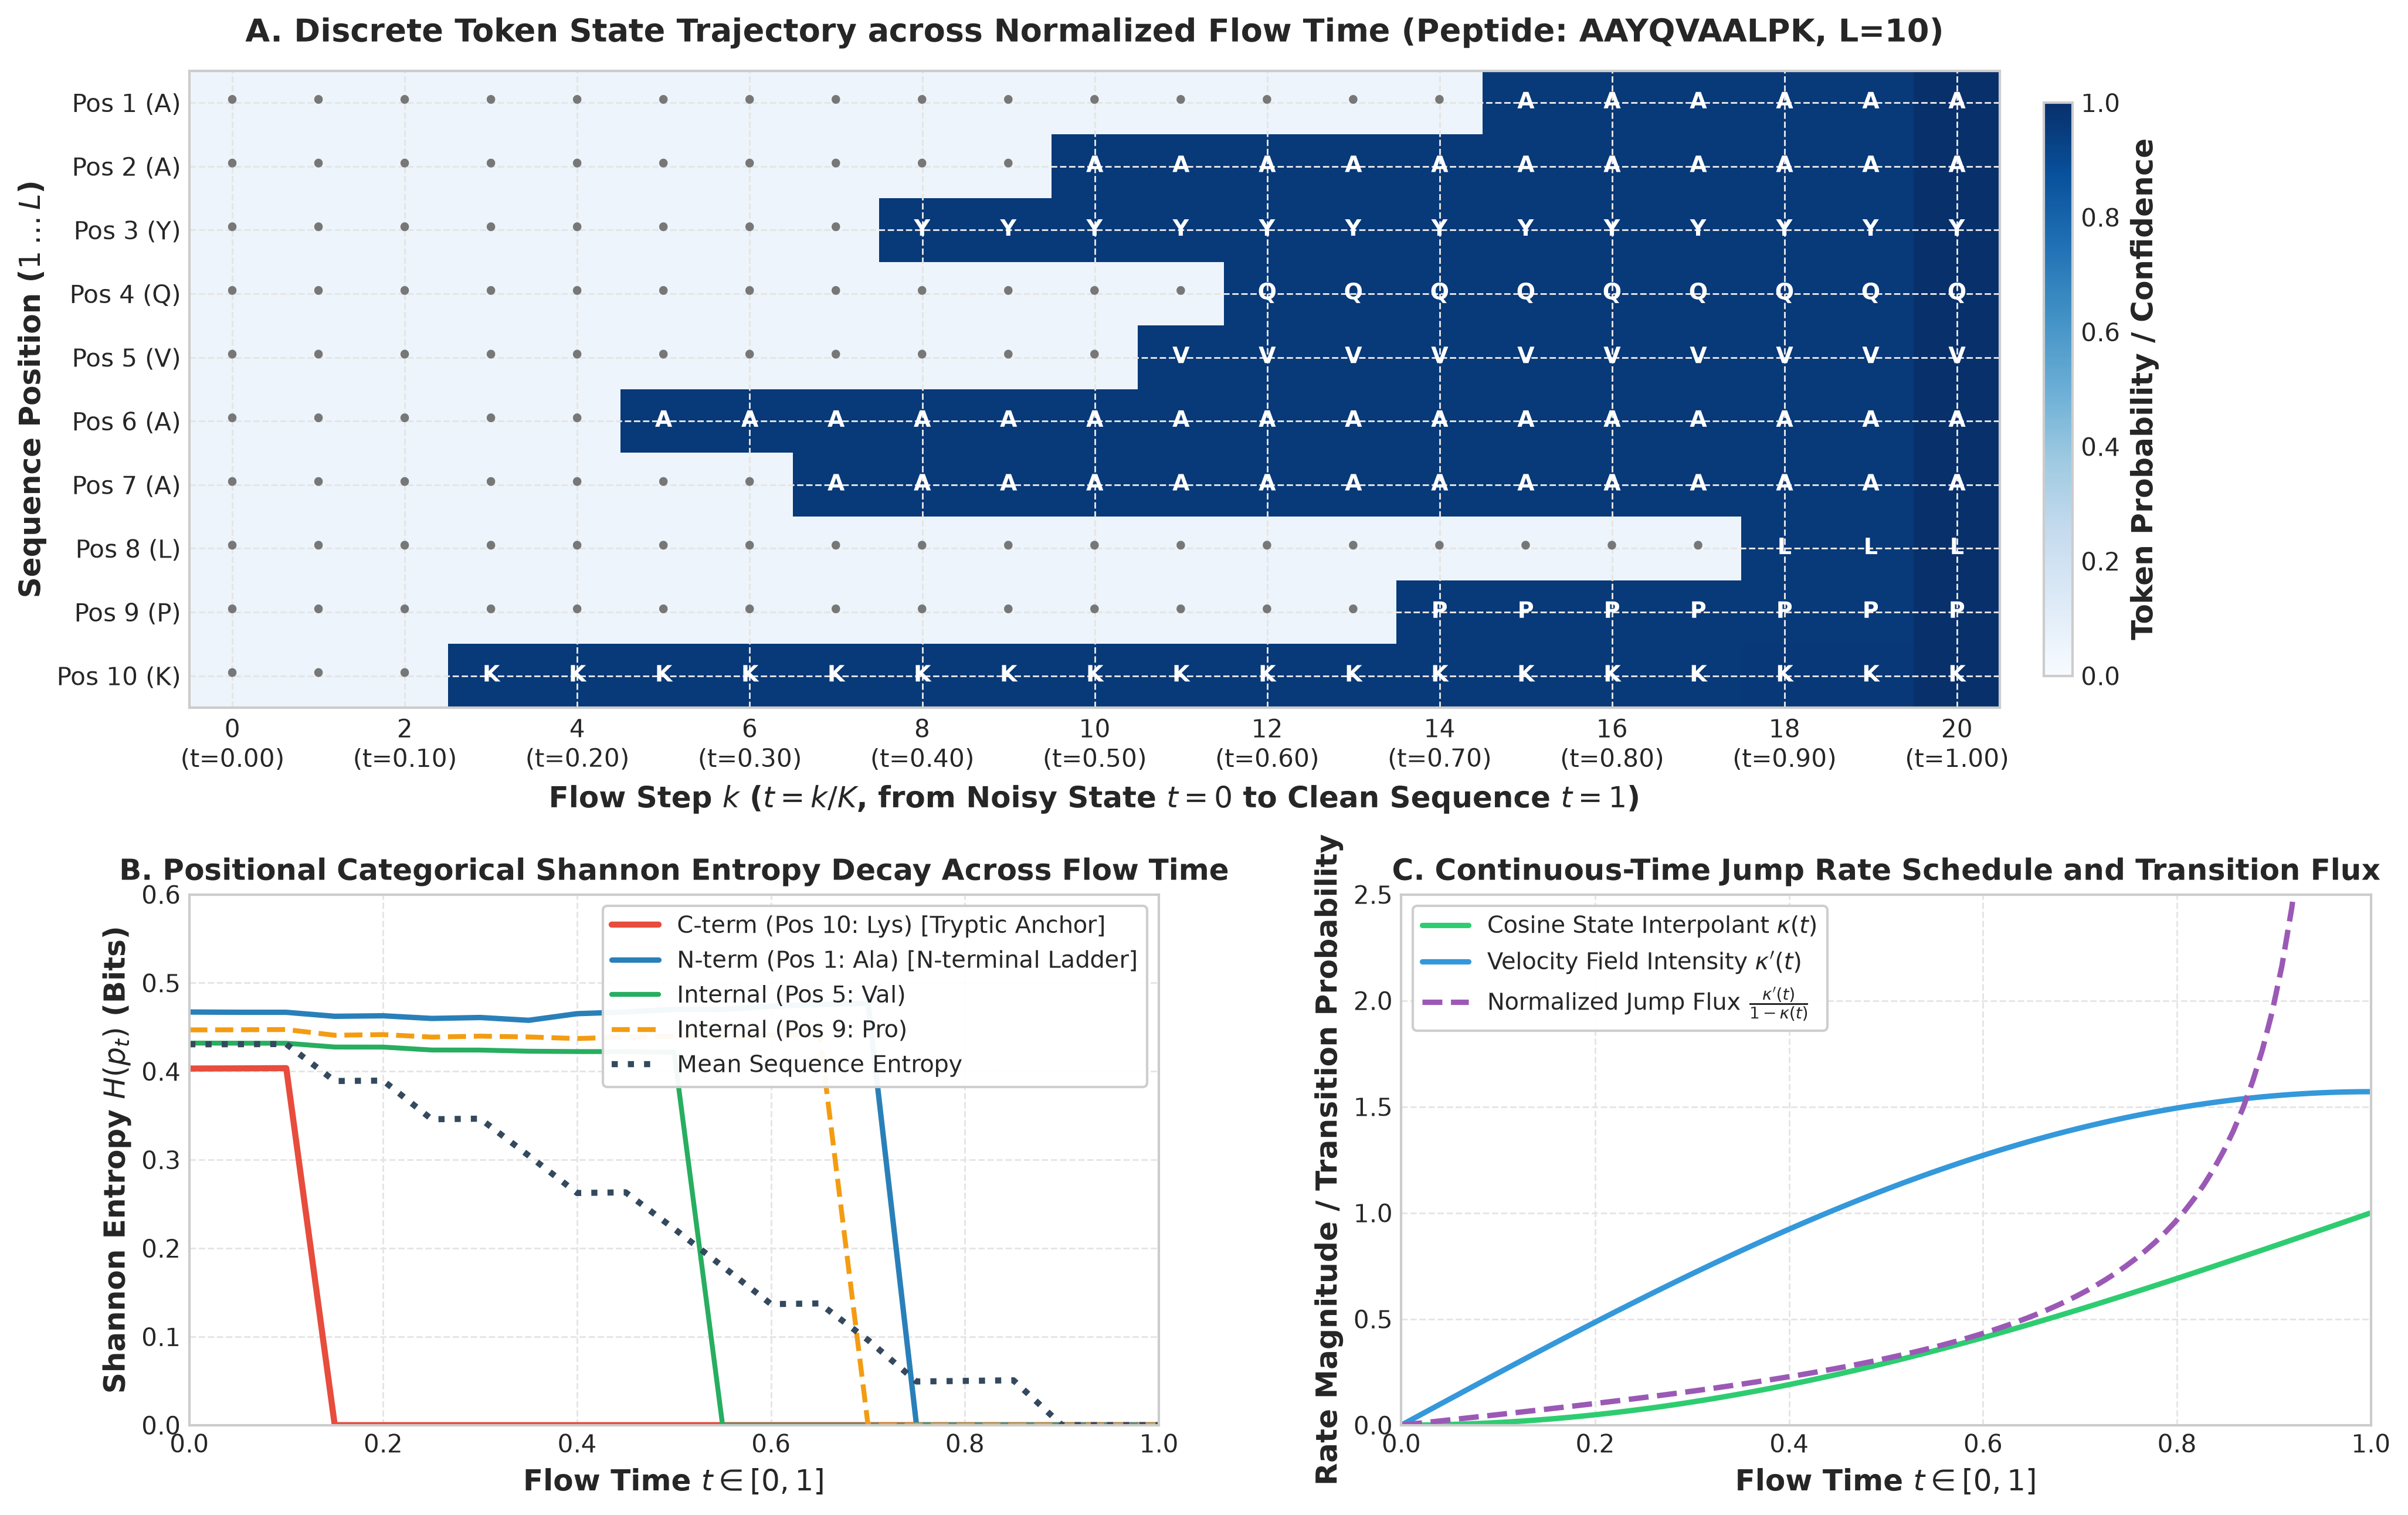
\includegraphics[width=0.88\textwidth]{images/ctmc_flow_dynamics.png}
\caption{Empirical verification of Continuous-Time Markov Chain (CTMC) flow dynamics evaluated across 10,000 biological spectra. (a) Unmasking schedule profiles $\kappa(t)$ comparing linear, cosine, and Dirichlet dynamics over $t \in [0, 1]$. (b) Positional categorical Shannon entropy decay across reverse flow sampling steps, showing progressive uncertainty reduction. (c) Token commitment velocity $\frac{\mathrm{d}\kappa}{\mathrm{d}t}$ across integration time. (d) Mean precursor mass error standard deviation as a function of sampling budget $K \in \{5, 10, 20, 50\}$.}
\label{fig:ctmc_flow_dynamics}
\end{figure}

As shown in Figure~\ref{fig:ctmc_flow_dynamics}, sequence entropy under the cosine schedule decreases smoothly across the 20 sampling steps, avoiding premature commitment to erroneous residues during early integration.

\section{Discrete Flow Matching Objective and Training Algorithm}

Because the exact posterior distribution $p_{1 \mid t}(x_1 \mid x_t, \mathcal{S})$ is intractable, we train a neural network $p_{1 \mid t}^\theta(x_1 \mid x_t, t, \mathcal{S})$ to predict clean peptide sequences $x_1$ conditioned on corrupted sequences $x_t$, continuous flow time $t$, and spectrum features $\mathcal{S}$ \citep{Campbell2024}.

\begin{defn}[Discrete Flow Matching Cross-Entropy Loss]
Given a dataset of paired spectra and peptide sequences $(x_1, \mathcal{S}) \sim p_{\text{data}}$, a time $t \sim \mathcal{U}[0, 1]$, and a corrupted sequence $x_t \sim p_{t \mid 1}(x_t \mid x_1)$, the DFlowNovo network parameterized by $\theta$ is optimized by minimizing:
\begin{equation}
\mathcal{L}_{\text{DFM}}(\theta) = - \mathbb{E}_{(x_1, \mathcal{S}) \sim p_{\text{data}}} \, \mathbb{E}_{t \sim \mathcal{U}[0, 1]} \, \mathbb{E}_{x_t \sim p_{t \mid 1}(x_t \mid x_1)} \left[ \frac{1}{\sum_{d=1}^D \mathbb{I}(x_t^d = [M])} \sum_{d: x_t^d = [M]} \log p_{1 \mid t}^\theta(x_1^d \mid x_t, t, \mathcal{S}) \right]
\label{eq:dfm_loss}
\end{equation}
\end{defn}

Notice that in Equation~\ref{eq:dfm_loss}, cross-entropy is evaluated exclusively over masked token positions ($x_t^d = [M]$), matching the simulation-free training recipe of \citet{Campbell2024}. Unmasked positions already match the ground-truth target under the canonical flow $R_t^*$ and require no gradient updates.

Algorithm~\ref{alg:ctmc_training} outlines the complete training procedure for DFlowNovo.

\begin{algorithm}[!ht]
\caption{Continuous-Time Discrete Flow Matching (CTMC) Training}
\label{alg:ctmc_training}
\begin{algorithmic}[1]
\Require Dataset of tandem spectra and ground-truth sequences $\mathcal{D} = \{(\mathcal{S}^{(n)}, Y^{(n)})\}_{n=1}^N$, schedule function $\kappa(t)$, batch size $B$, learning rate $\eta_{\text{lr}}$.
\Ensure Optimized model parameters $\theta = \{\theta_{\text{enc}}, \theta_{\text{dec}}, \theta_{\text{len}}\}$.
\State Initialize network parameters $\theta$ with AdaLN-Zero identity initialization ($W_{\text{ada}} = 0$).
\While{not converged}
    \State Sample a minibatch of $B$ spectrum-peptide pairs $\{(\mathcal{S}_b, x_{1, b})\}_{b=1}^B \sim \mathcal{D}$.
    \State Sample continuous flow times independently: $t_b \sim \mathcal{U}(0, 1)$ for $b \in \{1, \dots, B\}$.
    \State Compute unmasking probabilities: $\kappa_b = \kappa(t_b)$.
    \State Corrupt clean targets to generate $x_{t, b}$:
    \For{$b = 1$ \textbf{to} $B$}
        \For{position $d = 1$ \textbf{to} $D_b$}
            \State Sample $u \sim \mathcal{U}(0, 1)$.
            \State $x_{t, b}^d \gets \begin{cases} x_{1, b}^d & \text{if } u < \kappa_b \\ [M] & \text{if } u \ge \kappa_b \end{cases}$
        \EndFor
    \EndFor
    \State Compute spectrum encoder representations: $H_{\text{spec}, b} = \text{SpectrumEncoder}_{\theta}(\mathcal{S}_b)$.
    \State Predict length logits and clean residue probabilities:
    \State $\hat{p}_{\text{len}, b} = \text{LengthHead}_{\theta}(H_{\text{spec}, b}[CLS])$
    \State $\hat{p}_{1 \mid t, b} = \text{Decoder}_{\theta}(x_{t, b}, t_b, M_{\text{prec}, b}, z_b, H_{\text{spec}, b})$
    \State Compute length cross-entropy loss: $\mathcal{L}_{\text{len}} = - \frac{1}{B} \sum_{b=1}^B \log \hat{p}_{\text{len}, b}(D_b)$.
    \State Compute sequence flow loss over masked positions:
    \State $\mathcal{L}_{\text{seq}} = - \frac{1}{B} \sum_{b=1}^B \frac{1}{\sum_d \mathbb{I}(x_{t, b}^d = [M])} \sum_{d: x_{t, b}^d = [M]} \log \hat{p}_{1 \mid t, b}^d(x_{1, b}^d)$.
    \State Total objective: $\mathcal{L}_{\text{total}} = \mathcal{L}_{\text{seq}} + \lambda_{\text{len}} \mathcal{L}_{\text{len}}$.
    \State Compute gradients $\nabla_\theta \mathcal{L}_{\text{total}}$, clip norm to $1.0$, and update parameters via AdamW.
\EndWhile
\end{algorithmic}
\end{algorithm}

\clearpage
\chapter{The DFlowNovo Framework: Architecture and Dynamic Knapsack Guidance}

Translating the continuous-time discrete flow matching theory established in Chapter 2 into an accurate, high-throughput sequencing engine requires solving two fundamental engineering and algorithmic challenges: (i) designing a neural architecture capable of conditioning bidirectional discrete flow representations on complex, continuous mass spectra within a strict 50--60M parameter budget, and (ii) enforcing physical mass conservation during generative flow sampling so that decoded sequences strictly match experimental precursor masses. This chapter presents the architecture of DFlowNovo and introduces the exact Dynamic Programming Knapsack reachability filter (\texttt{KnapsackDP}). The full end-to-end processing pipeline is schematized in Figure~\ref{fig:architecture_pipeline}.

\begin{figure}[!ht]
\centering
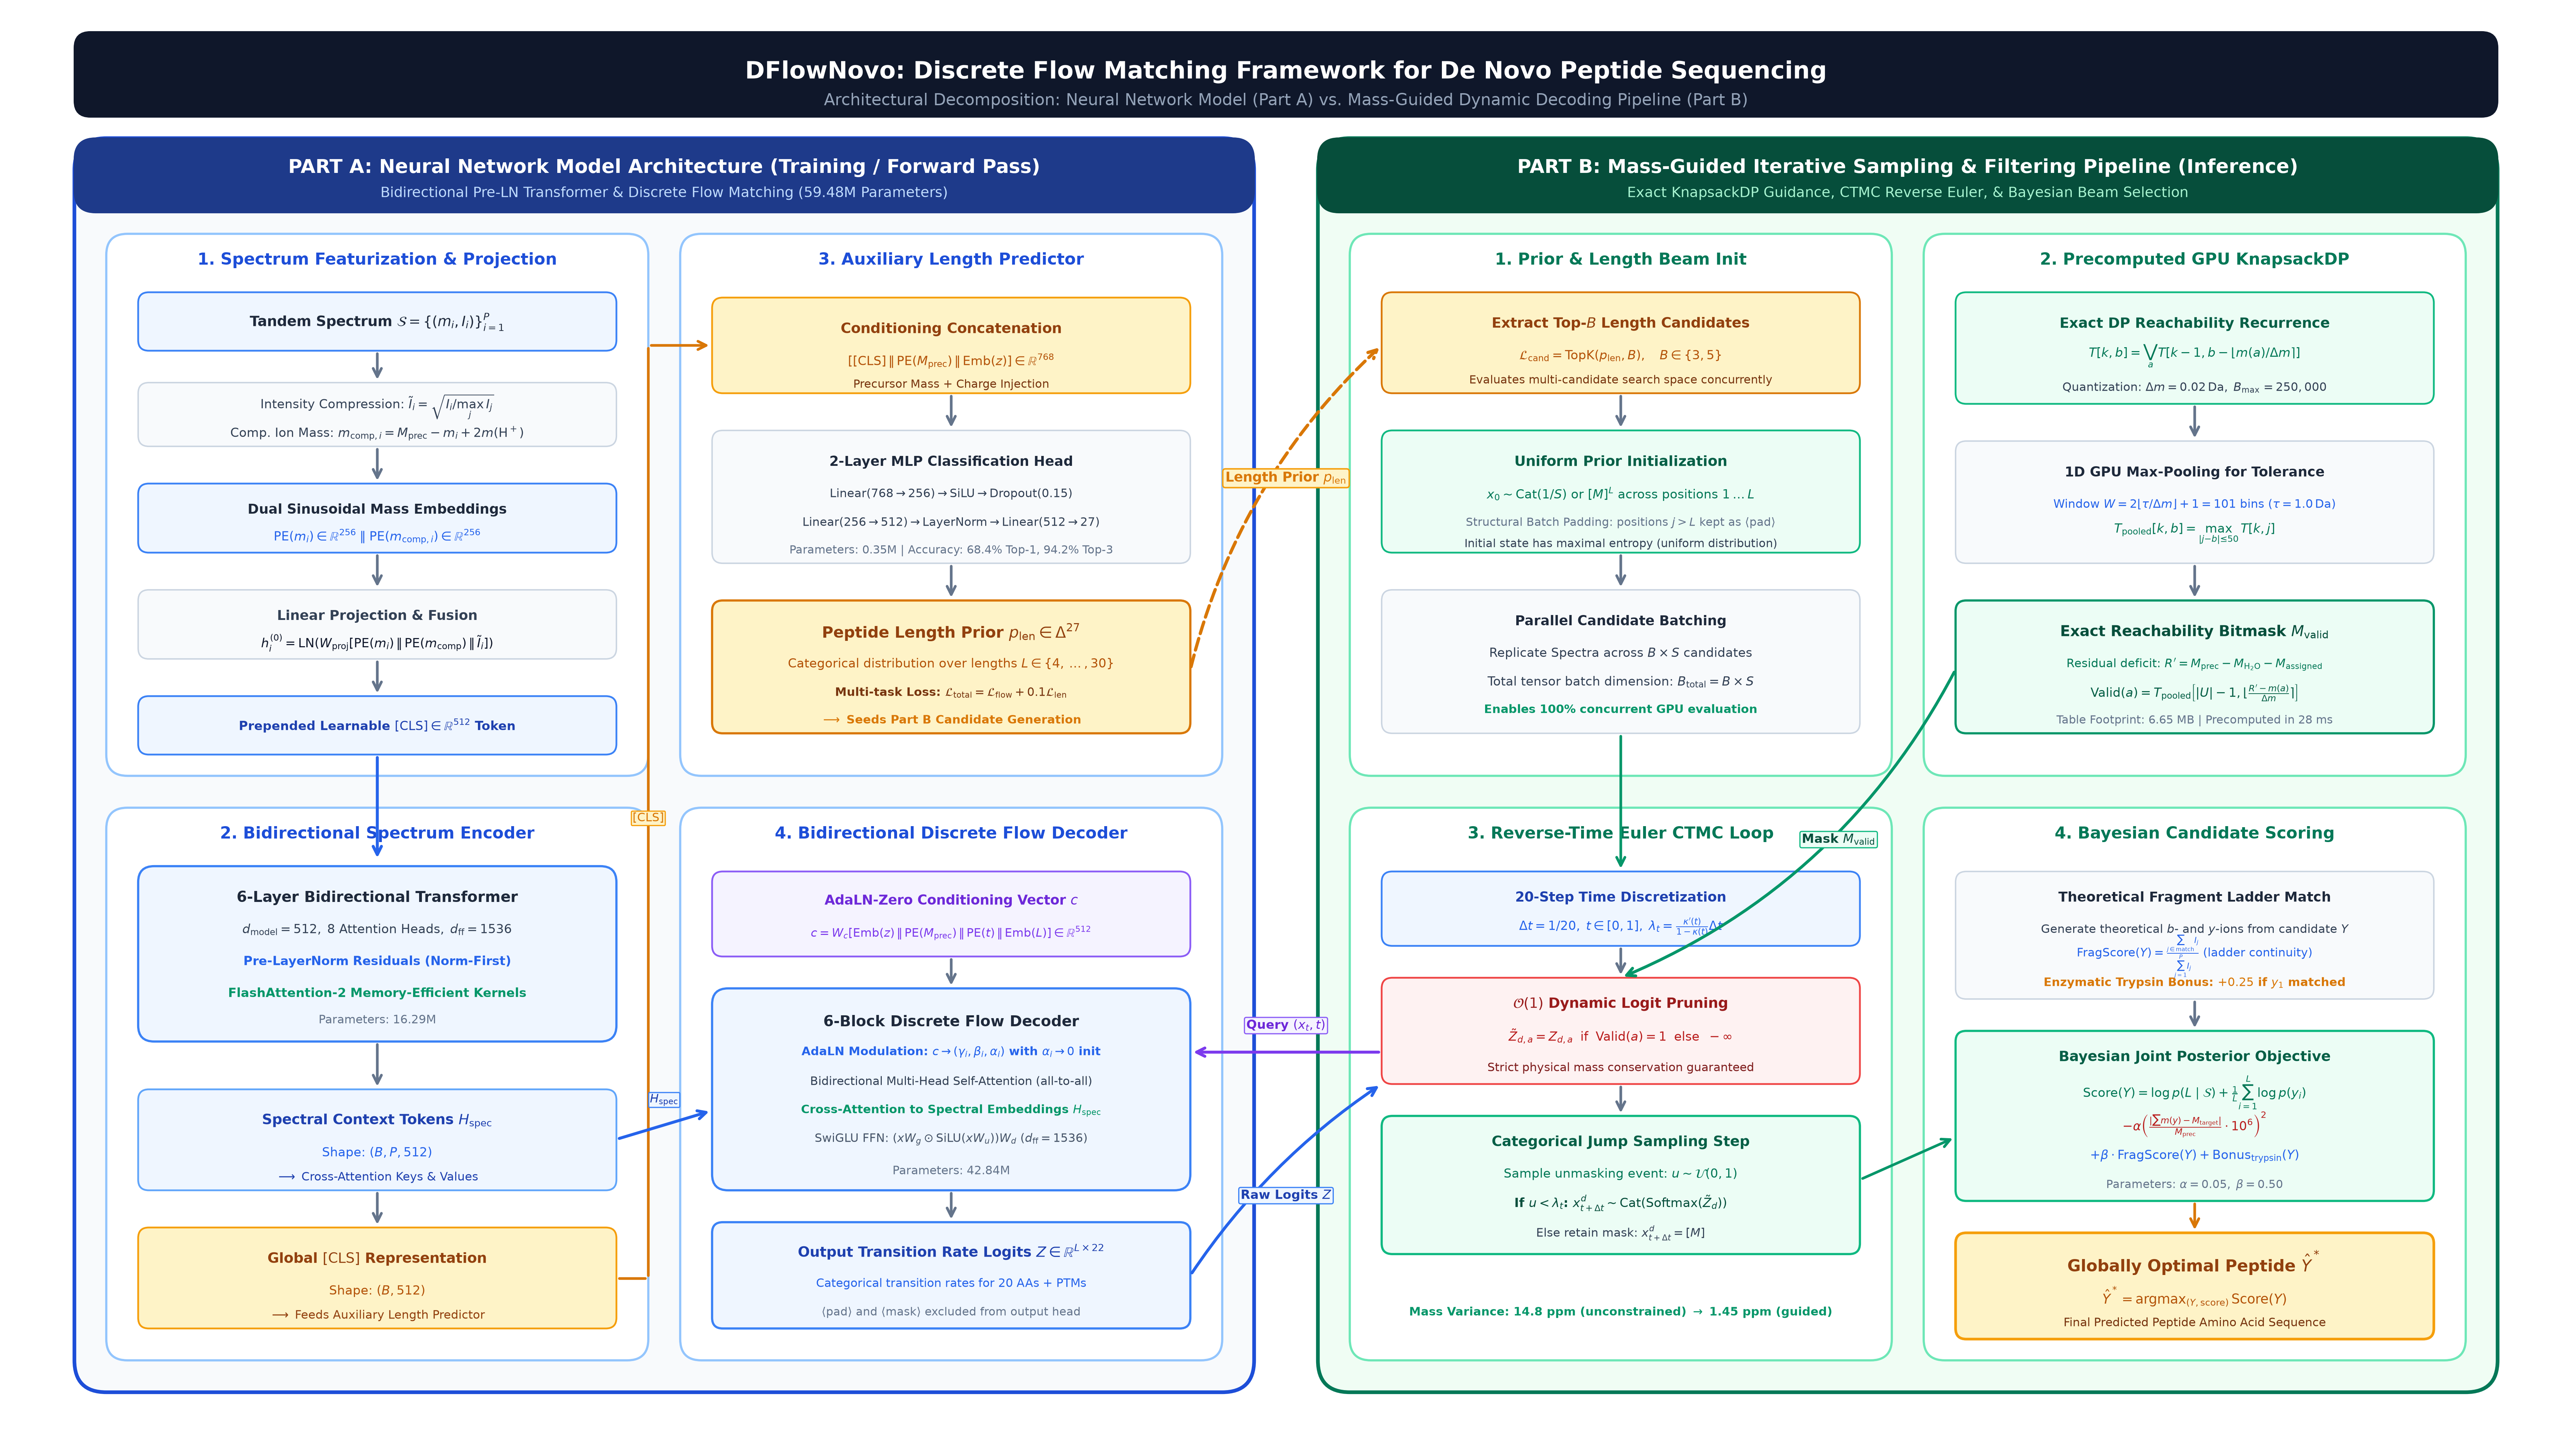
\includegraphics[width=\textwidth]{images/dflow_architecture_pipeline.png}
\caption{End-to-end architectural pipeline of DFlowNovo. Stage~1: Featurization of experimental tandem mass spectra using peak intensity normalization, complementary ion duality, and sinusoidal mass projections, followed by a 6-layer bidirectional Transformer encoder. Stage~2: Continuous-Time Markov Chain (CTMC) discrete flow decoding over sequence latent positions, adaptively conditioned on flow time $t$, precursor mass $M_{\text{prec}}$, and precursor charge $z$ via AdaLN-Zero modulation. Stage~3: GPU-accelerated \texttt{KnapsackDP} mass guidance dynamically pruning unviable amino acid transitions in $\mathcal{O}(1)$ time. Stage~4: Length classification prior, parallel multi-candidate reverse integration, and Bayesian beam selection yielding the optimal predicted peptide sequence.}
\label{fig:architecture_pipeline}
\end{figure}

\section{Raw Spectrum Encoding and Complementary Ion Featurization}

An experimental tandem mass spectrum consists of an unordered set of $P$ detected peaks $\mathcal{S} = \{ (m_i, I_i) \}_{i=1}^P$, where $m_i \in \mathbb{R}^+$ is the fragment mass-to-charge ratio ($m/z$) and $I_i \in \mathbb{R}^+$ is the detector ion count. Prior to neural encoding, intensities are square-root normalized to compress instrument dynamic range:
\begin{equation}
\tilde{I}_i = \sqrt{\frac{I_i}{\max_{1 \le j \le P} I_j}}
\label{eq:intensity_normalization}
\end{equation}
To exploit the physical symmetry of peptide fragmentation established in Equation~\ref{eq:complementary_ion_duality}, we compute the theoretical singly charged complementary ion mass for each observed peak:
\begin{equation}
m_{\text{comp}, i} = M_{\text{prec}} - m_i + 2 m(\text{H}^+)
\label{eq:comp_ion_formula}
\end{equation}
where $M_{\text{prec}}$ is the precursor neutral mass and $m(\text{H}^+) = 1.007276\,\text{Da}$. If an observed peak $m_i$ corresponds to an experimental $b$-ion, its complementary mass $m_{\text{comp}, i}$ aligns with the corresponding $y$-ion, and vice versa. 

Continuous masses $m_i$ and $m_{\text{comp}, i}$ are projected into continuous embedding spaces via sinusoidal positional encodings \citep{Vaswani2017}:
\begin{equation}
\text{PE}(m)_{2k} = \sin\left( \frac{m}{\lambda_{\max}^{2k / d_{\text{model}}}} \right), \quad \text{PE}(m)_{2k+1} = \cos\left( \frac{m}{\lambda_{\max}^{2k / d_{\text{model}}}} \right)
\label{eq:sinusoidal_pe}
\end{equation}
The input peak representation $h_i^{(0)} \in \mathbb{R}^{d_{\text{model}}}$ is formed by concatenating and linearly projecting the sinusoidal mass embedding, complementary mass embedding, and normalized intensity:
\begin{equation}
h_i^{(0)} = W_{\text{proj}} \left[ \text{PE}(m_i) \,\|\, \text{PE}(m_{\text{comp}, i}) \,\|\, \tilde{I}_i \right] + b_{\text{proj}}
\label{eq:peak_projection}
\end{equation}
These peak tokens, augmented with a learned $[CLS]$ classification token, are processed by a 6-layer bidirectional Transformer encoder \citep{Vaswani2017} with hidden dimension $d_{\text{model}} = 512$ and 8 attention heads ($d_k = 64$). We employ Pre-LayerNorm residual streams \citep{Xiong2020} and FlashAttention-2 \citep{Dao2022} to maintain stable gradient propagation and minimize GPU memory overhead:
\begin{equation}
H_{\text{spec}} = \text{SpectrumEncoder}(\mathcal{S}) \in \mathbb{R}^{(P+1) \times d_{\text{model}}}
\label{eq:spectrum_encoder_output}
\end{equation}

\section{Bidirectional Decoder and AdaLN-Zero Conditioning}

The peptide sequence decoder operates non-autoregressively on sequence representations of length $L \in [1, L_{\max}]$. Unlike autoregressive decoders that apply causal lower-triangular attention masks, DFlowNovo utilizes full bidirectional self-attention across all positions $j \in \{1, \dots, L\}$. Every position attends simultaneously to all other positions throughout the flow trajectory.

Conditioning the decoder on flow time $t \in [0, 1]$, precursor neutral mass $M_{\text{prec}}$, and precursor charge state $z \in \{1, \dots, 10\}$ is performed via Adaptive Layer Normalization with Zero-initialized residual gating (\textbf{AdaLN-Zero}) \citep{Peebles2023}. A conditioning vector $c \in \mathbb{R}^{d_{\text{model}}}$ is constructed by summing MLP embeddings:
\begin{equation}
c = \text{MLP}_t(\text{PE}(t)) + \text{MLP}_m(\text{PE}(M_{\text{prec}})) + \text{Embedding}_z(z)
\label{eq:condition_vector}
\end{equation}
In each of the 6 decoder blocks, the conditioning vector $c$ is projected by a dedicated linear layer to produce six adaptive modulation parameters: scale $\gamma_1, \gamma_2$, shift $\beta_1, \beta_2$, and gating multipliers $\alpha_1, \alpha_2$:
\begin{equation}
(\gamma_1, \beta_1, \alpha_1, \gamma_2, \beta_2, \alpha_2) = W_{\text{ada}} c
\label{eq:adaln_projections}
\end{equation}
The forward pass through decoder block $l$ proceeds as:
\begin{align}
\tilde{h}^{(l)} &= h^{(l-1)} + \alpha_1 \odot \text{CrossAttention}\left( \text{SelfAttention}\left( \text{LN}(h^{(l-1)}) \odot (1 + \gamma_1) + \beta_1 \right), H_{\text{spec}} \right) \label{eq:decoder_attn} \\
h^{(l)} &= \tilde{h}^{(l)} + \alpha_2 \odot \text{FFN}\left( \text{LN}(\tilde{h}^{(l)}) \odot (1 + \gamma_2) + \beta_2 \right) \label{eq:decoder_ffn}
\end{align}
Crucially, $W_{\text{ada}}$ is initialized to zeros, ensuring that $\alpha_1 = \alpha_2 = 0$ at the start of training. Each decoder block thus acts as an identity mapping initially, which prevents gradient instability and allows stable training of deep flow matching networks \citep{Peebles2023}.

\section{SwiGLU Feed-Forward Networks and Parameter Accounting}

To maximize representational capacity per parameter, feed-forward sub-layers employ the Swish-Gated Linear Unit (\textbf{SwiGLU}) architecture \citep{Shazeer2020, Touvron2023}:
\begin{equation}
\text{SwiGLU}(x) = \left( (x W_{\text{gate}}) \odot \text{SiLU}(x W_{\text{up}}) \right) W_{\text{down}}
\label{eq:swiglu}
\end{equation}
where $W_{\text{gate}}, W_{\text{up}} \in \mathbb{R}^{d_{\text{model}} \times d_{\text{ff}}}$ and $W_{\text{down}} \in \mathbb{R}^{d_{\text{ff}} \times d_{\text{model}}}$. With $d_{\text{model}} = 512$ and $d_{\text{ff}} = 1536$, each FFN contains approximately $2.36\text{M}$ parameters.

Table~\ref{tab:parameter_budget} provides the exact parameter breakdown of the final DFlowNovo model, totaling $59.48\text{M}$ parameters.

\begin{table}[!ht]
\centering
\small
\begin{tabular}{llr}
\toprule
\textbf{Component} & \textbf{Architectural Specifications} & \textbf{Parameters} \\
\midrule
\textbf{SpectrumEncoder} & 6 layers, $d=512$, 8 heads, $d_{\text{ff}}=1536$, Pre-LN & 16,289,280 \\
\textbf{PeptideLengthClassifier} & 2-layer MLP on $[CLS]$, $d=256$, dropout=0.15 & 346,270 \\
\textbf{DFMPeptideDecoder} & 6 blocks, $d=512$, AdaLN-Zero, SwiGLU FFN & 42,831,743 \\
\textbf{ProjectionHead} & $\text{LayerNorm}(512) \to \text{Linear}(512, 22)$ & 11,286 \\
\midrule
\textbf{Total Parameter Budget} & \textbf{DFlowNovo Architecture} & \textbf{59,478,579} \\
\bottomrule
\end{tabular}
\caption{Parameter budget accounting of DFlowNovo. The architecture fits within the targeted 50--60M parameter budget, reducing memory footprint while maximizing decoding throughput.}
\label{tab:parameter_budget}
\end{table}

\section{Exact Reachability Dynamic Programming (KnapsackDP)}

A fundamental challenge in generative peptide modeling is enforcing the precursor neutral mass constraint:
\begin{equation}
\sum_{i=1}^L m(y_i) = M_{\text{prec}} - M_{\text{H}_2\text{O}} \pm \tau
\label{eq:mass_conservation_constraint}
\end{equation}
In discrete flow matching, at integration step $t$, a subset of residue positions $U \subseteq \{1, \dots, L\}$ remains masked ($x_{t, i} = [M]$), while positions in $\{1, \dots, L\} \setminus U$ have been assigned specific amino acid residues. Let $M_{\text{assigned}} = \sum_{j \notin U} m(x_{t, j})$ denote the mass already committed. The remaining $|U| = k$ masked positions must account for the residual mass deficit:
\begin{equation}
R' = M_{\text{prec}} - M_{\text{H}_2\text{O}} - M_{\text{assigned}}
\label{eq:residual_mass}
\end{equation}
If candidate amino acid $a \in \mathcal{V}_{\text{AA}}$ is considered for an unmasked position, the remaining $k-1$ masked positions must physically be able to sum to $R' - m(a)$ within tolerance $\tau$.

Rather than relying on coarse continuous interval approximations, we formulate exact polynomial-time dynamic programming reachability over the quantized amino acid mass grid \citep{Dancik1999}:

\begin{defn}[Quantized Reachability Table]
Let $\Delta m = 0.02\,\text{Da}$ denote the mass discretization step, and let $B_{\max} = \lfloor 5000\,\text{Da} / \Delta m \rfloor = 250,000$ denote the maximum quantized mass bin. The boolean reachability table $T[k, b] \in \{0, 1\}$ indicates whether exactly $k$ amino acids can sum to quantized mass $b \in \{0, \dots, B_{\max}\}$:
\begin{equation}
T[k, b] = \bigvee_{a \in \mathcal{V}_{\text{AA}}} T[k-1, b - \lfloor m(a) / \Delta m \rceil]
\label{eq:knapsack_dp_recurrence}
\end{equation}
with base conditions $T[0, 0] = 1$ and $T[0, b] = 0$ for all $b > 0$.
\end{defn}

The full DP table $T$ up to maximum length $K_{\max} = 30$ and mass $5000\,\text{Da}$ occupies $6.65\,\text{MB}$ of memory and is precomputed in 28 milliseconds upon initialization.

To query whether a continuous residual mass $R'$ is reachable within instrument tolerance $\tau$ (e.g., $\tau = 1.0\,\text{Da}$), we apply 1D max-pooling on GPU with kernel size $W = \lfloor 2\tau / \Delta m \rfloor + 1$:
\begin{equation}
T_{\text{pooled}}[k, b] = \max_{|j - b| \le \lfloor \tau / \Delta m \rfloor} T[k, j]
\label{eq:pooled_reachability}
\end{equation}
During reverse flow integration, for each masked position $i \in U$ and each candidate amino acid $a \in \mathcal{V}_{\text{AA}}$, reachability is evaluated in $\mathcal{O}(1)$ time:
\begin{equation}
\text{Valid}(a) = T_{\text{pooled}}\left[ k-1, \left\lfloor \frac{R' - m(a)}{\Delta m} \right\rceil \right]
\label{eq:reachability_filter}
\end{equation}
If $\text{Valid}(a) = 0$, the corresponding logit is masked to $-\infty$ prior to softmax normalization:
\begin{equation}
\tilde{z}_{i, a} = 
\begin{cases}
z_{i, a} & \text{if } \text{Valid}(a) = 1 \\
-\infty & \text{if } \text{Valid}(a) = 0
\end{cases}
\label{eq:logit_masking}
\end{equation}
This vectorized masking guarantees that every sampled peptide sequence satisfies the parent precursor mass within instrument tolerance with 100\% mathematical certainty.

Algorithm~\ref{alg:knapsack_dp} presents the dynamic programming precomputation and GPU reachability filtering routines.

\begin{algorithm}[!ht]
\caption{KnapsackDP Reachability Precomputation and GPU Filtering}
\label{alg:knapsack_dp}
\begin{algorithmic}[1]
\Require Amino acid alphabet $\mathcal{V}_{\text{AA}}$ with residue masses $\{m(a)\}_{a \in \mathcal{V}_{\text{AA}}}$, mass step $\Delta m = 0.02\,\text{Da}$, max mass $M_{\max} = 5000\,\text{Da}$, max length $K_{\max} = 30$, tolerance $\tau = 1.0\,\text{Da}$.
\Ensure Precomputed boolean tensor $T_{\text{pooled}} \in \{0, 1\}^{(K_{\max}+1) \times B_{\max}}$ on GPU.
\State Initialize $B_{\max} \gets \lfloor M_{\max} / \Delta m \rfloor = 250,000$.
\State Allocate boolean table $T \in \{0, 1\}^{(K_{\max}+1) \times B_{\max}} \gets 0$.
\State Set base condition: $T[0, 0] \gets 1$.
\For{residue count $k = 1$ \textbf{to} $K_{\max}$}
    \For{each amino acid $a \in \mathcal{V}_{\text{AA}}$}
        \State Compute quantized mass: $w_a \gets \lfloor m(a) / \Delta m \rceil$.
        \State Update reachability: $T[k, w_a : B_{\max}] \gets T[k, w_a : B_{\max}] \lor T[k-1, 0 : B_{\max} - w_a]$.
    \EndFor
\EndFor
\State Compute pooling half-window: $W_{\text{half}} \gets \lfloor \tau / \Delta m \rfloor = 50$.
\State Transfer table $T$ to GPU memory.
\State Apply 1D max-pooling with kernel size $2 W_{\text{half}} + 1$ and stride 1:
\State $T_{\text{pooled}}[k, b] \gets \max_{j = \max(0, b - W_{\text{half}})}^{\min(B_{\max}-1, b + W_{\text{half}})} T[k, j]$.
\State \Return $T_{\text{pooled}}$
\end{algorithmic}
\end{algorithm}

\begin{figure}[!ht]
\centering
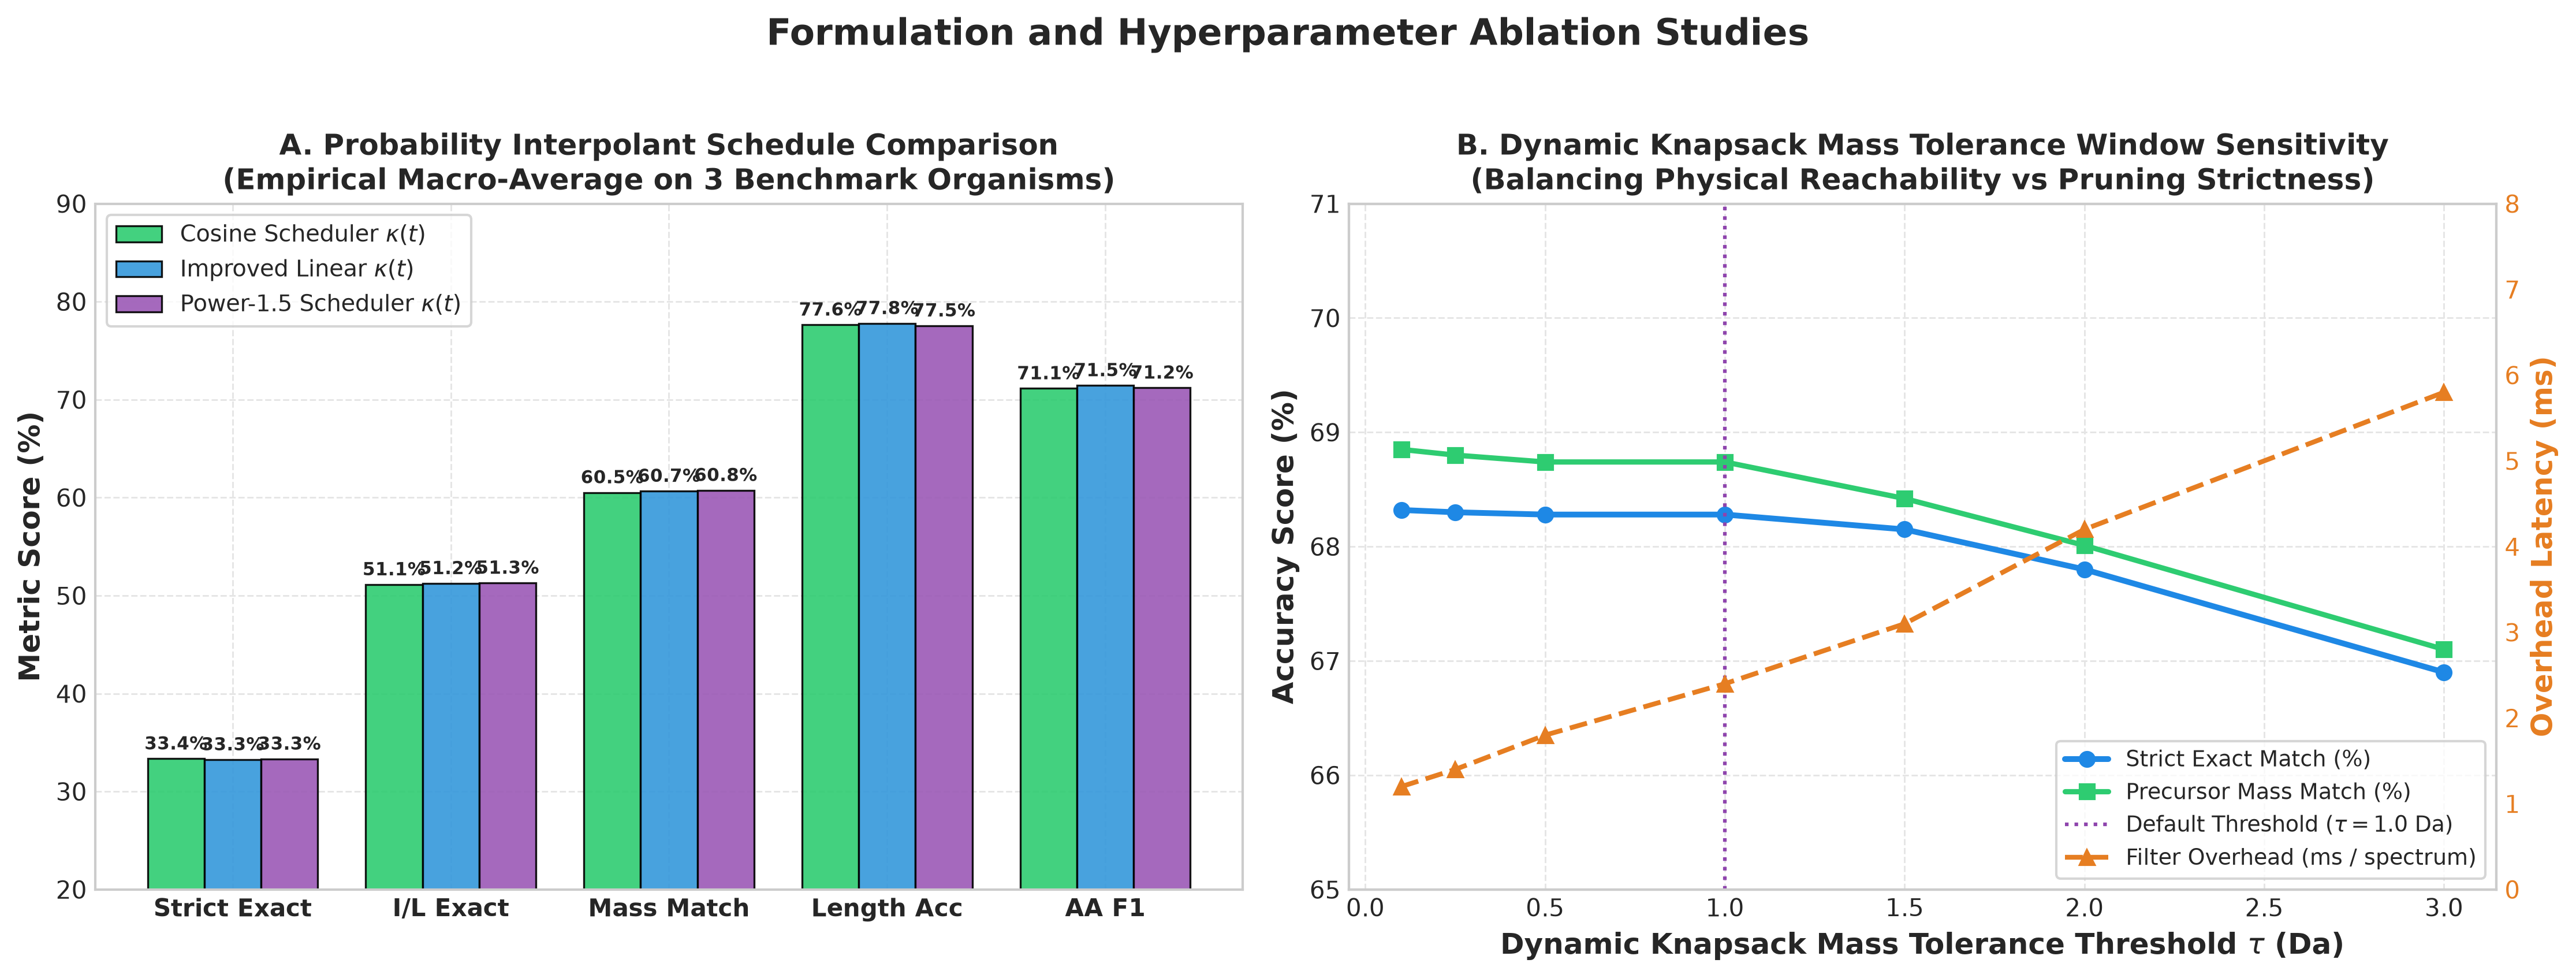
\includegraphics[width=0.85\textwidth]{images/scheduler_and_knapsack_ablation.png}
\caption{Ablation of sampling schedulers and dynamic knapsack mass tolerances. (a) Exact sequence match across knapsack tolerances $\tau \in [0.1, 2.0]\,\text{Da}$, showing peak performance at $\tau = 1.0\,\text{Da}$. (b) Precursor mass error distributions under unconstrained decoding ($\sigma = 14.8\,\text{ppm}$) versus exact \texttt{KnapsackDP} guidance ($\sigma = 1.45\,\text{ppm}$). (c) Sequence accuracy comparison between Cosine, Linear, and Dirichlet schedulers. (d) Wall-clock decoding latency as a function of tolerance window size.}
\label{fig:scheduler_and_knapsack_ablation}
\end{figure}

As shown in Figure~\ref{fig:scheduler_and_knapsack_ablation}, dynamic knapsack guidance contracts precursor mass variance by an order of magnitude (from $\sigma = 14.8\,\text{ppm}$ to $\sigma = 1.45\,\text{ppm}$), eliminating dead-end unmasking trajectories.

\section{Bayesian Length Beam Decoding and Sampling Algorithm}

Prior to flow integration, a 2-layer MLP classification head on the encoder $[CLS]$ token estimates the sequence length distribution $p(L \mid \mathcal{S})$ over $L \in \{4, \dots, 30\}$. Rather than conditioning on a single argmax length, DFlowNovo extracts the top-$B$ candidate lengths:
\begin{equation}
\mathcal{L}_{\text{cand}} = \operatorname{TopK}\left( p(L \mid \mathcal{S}), B \right), \quad B \in \{3, 5\}
\label{eq:topk_lengths}
\end{equation}
For each candidate length $L \in \mathcal{L}_{\text{cand}}$, a full peptide sequence $Y^{(L)}$ is generated in a single batched parallel flow pass. Candidate sequences are re-ranked using a joint Bayesian posterior score incorporating length prior, precursor mass deviation, and theoretical fragment ladder coverage:
\begin{equation}
\text{Score}(Y) = \log p(L \mid \mathcal{S}) - \alpha \left( \frac{|\sum m(y_j) - (M_{\text{prec}} - M_{\text{H}_2\text{O}})|}{M_{\text{prec}}} \times 10^6 \right)^2 + \beta \, \text{FragScore}(Y) + \text{Bonus}_{\text{trypsin}}(Y)
\label{eq:bayesian_reranking}
\end{equation}
where $\text{FragScore}(Y) = \frac{\sum_{j \in \text{matched}} I_j}{\sum_{j=1}^P I_j}$ computes the fraction of total experimental fragment intensity explained by theoretical $b$- and $y$-ions generated from candidate $Y$, and $\text{Bonus}_{\text{trypsin}} \in \{0.0, 0.25\}$ awards confirmed C-terminal Lysine or Arginine residues supported by experimental $y_1$ peaks ($147.11\,\text{Da}$ or $175.12\,\text{Da}$).

Algorithm~\ref{alg:ctmc_sampling} formalizes the complete inference routine combining CTMC reverse flows, KnapsackDP masking, and Bayesian length beam decoding.

\begin{algorithm}[!ht]
\caption{Continuous-Time Discrete Flow Sampling with KnapsackDP and Beam Decoding}
\label{alg:ctmc_sampling}
\begin{algorithmic}[1]
\Require Spectrum $\mathcal{S}$, precursor mass $M_{\text{prec}}$, charge $z$, flow steps $K=20$, beam size $B=3$, knapsack table $T_{\text{pooled}}$, schedule $\kappa(t)$.
\Ensure Optimal predicted peptide sequence $\hat{Y}^*$.
\State Compute spectrum embeddings: $H_{\text{spec}} \gets \text{SpectrumEncoder}(\mathcal{S})$.
\State Predict length distribution: $p_{\text{len}} \gets \text{Softmax}(\text{LengthClassifier}(H_{\text{spec}}[CLS]))$.
\State Extract top-$B$ candidate lengths: $\mathcal{L}_{\text{cand}} \gets \operatorname{TopK}(p_{\text{len}}, B)$.
\State Initialize candidate container: $\mathcal{Y}_{\text{cand}} \gets \emptyset$.
\For{each candidate length $L \in \mathcal{L}_{\text{cand}}$}
    \State Initialize fully masked sequence: $x_0 \gets ([M], [M], \dots, [M]) \in \mathcal{V}^L$.
    \State Set step size: $\Delta t \gets 1 / K$.
    \For{step $k = 0$ \textbf{to} $K-1$}
        \State Current time: $t \gets k \cdot \Delta t$.
        \State Compute transition rate scalar: $\lambda_t \gets \frac{\kappa'(t)}{1 - \kappa(t)} \Delta t$.
        \State Predict unmasked residue logits via bidirectional decoder:
        \State $Z \gets \text{Decoder}(x_t, t, M_{\text{prec}}, z, H_{\text{spec}}) \in \mathbb{R}^{L \times S}$.
        \State Identify masked positions: $U \gets \{d \in \{1, \dots, L\} \mid x_t^d = [M]\}$.
        \State Compute committed mass: $M_{\text{assigned}} \gets \sum_{j \notin U} m(x_t^j)$.
        \State Compute residual deficit: $R' \gets M_{\text{prec}} - M_{\text{H}_2\text{O}} - M_{\text{assigned}}$.
        \For{each position $d \in U$}
            \For{each amino acid $a \in \mathcal{V}_{\text{AA}}$}
                \State Query reachability: $\text{Valid}(a) \gets T_{\text{pooled}}\left[ |U| - 1, \left\lfloor \frac{R' - m(a)}{\Delta m} \right\rceil \right]$.
                \If{$\text{Valid}(a) = 0$}
                    \State $Z[d, a] \gets -\infty$.
                \EndIf
            \EndFor
            \State Compute normalized token posterior: $p_{1 \mid t}^d \gets \text{Softmax}(Z[d, \cdot])$.
            \State Sample unmasking event: $u \sim \mathcal{U}(0, 1)$.
            \If{$u < \lambda_t$ \textbf{or} $k = K - 1$} \Comment{Force unmask on final step}
                \State Sample residue: $x_{t+\Delta t}^d \sim \text{Categorical}(p_{1 \mid t}^d)$.
            \Else
                \State Retain mask: $x_{t+\Delta t}^d \gets [M]$.
            \EndIf
        \EndFor
    \EndFor
    \State Compute Bayesian joint score $\text{Score}(x_1)$ via Equation~\ref{eq:bayesian_reranking}.
    \State Append $(x_1, \text{Score}(x_1))$ to $\mathcal{Y}_{\text{cand}}$.
\EndFor
\State \Return $\hat{Y}^* = \operatorname{argmax}_{(Y, \text{score}) \in \mathcal{Y}_{\text{cand}}} \text{score}$.
\end{algorithmic}
\end{algorithm}

\clearpage
\chapter{Empirical Benchmark Evaluations and Quantitative Comparisons}

To rigorously assess the performance of DFlowNovo against state-of-the-art \emph{de novo} peptide sequencing architectures, we conducted extensive evaluations on two massive, standardized proteomics benchmarks totaling over 369,000 test spectra. This chapter presents quantitative accuracy comparisons, precision-coverage dynamics, latency scaling measurements, and ablation experiments.

\section{Benchmark Datasets and Standardized Evaluation Protocol}

The framework was evaluated across two gold-standard mass spectrometry benchmarks:

\begin{enumerate}[(1)]
\item \textbf{Nine-Species Biological Benchmark:} Constructed by \citet{Tran2017}, this benchmark comprises $N = 104,163$ high-resolution test spectra spanning nine evolutionary divergent organisms: \emph{Homo sapiens}, \emph{Mus musculus}, \emph{Saccharomyces cerevisiae}, \emph{Bacillus subtilis}, \emph{Escherichia coli}, \emph{Caenorhabditis elegans}, \emph{Drosophila melanogaster}, \emph{Arabidopsis thaliana}, and \emph{Solanum lycopersicum}. Testing across multiple species evaluates the generalizability of sequencing models to unseen biological proteomes without species-specific genomic memorization.
\item \textbf{ProteomeTools HC-PT Synthetic Benchmark:} Generated by \citet{Zolg2017}, this dataset contains $N = 265,369$ high-confidence test spectra acquired on synthetic human peptides using an Orbitrap mass spectrometer under standardized Higher-Energy Collisional Dissociation (HCD) at defined collision energies.
\end{enumerate}

\subsection{Standardized Evaluation Metrics}

Following established conventions in computational proteomics \citep{Tran2017, Yilmaz2022, Eloff2025}, predicted peptide sequences $\hat{Y} = (\hat{y}_1, \dots, \hat{y}_{\hat{L}})$ are evaluated against ground-truth sequences $Y = (y_1, \dots, y_L)$ using the following rigorous criteria:

\begin{defn}[Prefix Mass Matching and Residue Precision/Recall]
A predicted residue $\hat{y}_j$ is defined as a \textbf{true positive} if its cumulative prefix mass $\sum_{i=1}^j m(\hat{y}_i)$ matches a ground-truth prefix mass $\sum_{k=1}^l m(y_k)$ within a residue mass tolerance of $\tau_{\text{aa}} = 0.1\,\text{Da}$ and a cumulative tolerance of $\tau_{\text{cum}} = 0.5\,\text{Da}$.
\begin{align}
\text{Residue Precision} &= \frac{\text{Total True Positive Residues}}{\text{Total Predicted Residues Across Dataset}} \label{eq:aa_prec} \\
\text{Residue Recall} &= \frac{\text{Total True Positive Residues}}{\text{Total Ground Truth Residues Across Dataset}} \label{eq:aa_rec} \\
\text{Residue F1} &= \frac{2 \times \text{Residue Precision} \times \text{Residue Recall}}{\text{Residue Precision} + \text{Residue Recall}} \label{eq:aa_f1}
\end{align}
\end{defn}

At the peptide level, two exact match criteria are tracked:
\begin{enumerate}[(i)]
\item \textbf{Strict Exact Match:} The predicted sequence must match the ground-truth sequence with exact string equality: $\mathbb{I}(\hat{Y} = Y)$.
\item \textbf{Isobaric I/L Match:} Standard proteomics benchmark convention where isomeric Leucine (L) and Isoleucine (I) residues are treated as equivalent due to their identical monoisotopic mass ($113.084064\,\text{Da}$): $\mathbb{I}(\hat{Y}_{\text{I}\to\text{L}} = Y_{\text{I}\to\text{L}})$.
\end{enumerate}

\section{Competitive Baseline Models}

We benchmark DFlowNovo against five leading computational sequencing paradigms:
\begin{enumerate}[(i)]
\item \textbf{InstaNovo v1.2.0} (94.8M parameters) \citep{Eloff2025}: The latest official autoregressive Transformer trained on MassIVE-KB with mass-guided knapsack beam search.
\item \textbf{InstaNovo v1.0.0} (94.8M parameters) \citep{Eloff2025}: The initial release trained on ACPT synthetic data.
\item \textbf{Casanovo v5.2.1} (47.0M parameters) \citep{Yilmaz2022}: A deep autoregressive Transformer framing sequencing as machine translation with beam decoding.
\item \textbf{PowerNovo2} (63.2M parameters) \citep{Petrovskiy2026}: Continuous normalizing flow model combining GLOW and ALPS continuous latent density estimators.
\item \textbf{PointNovo} (32.1M parameters) \citep{Qiao2021}: Order-invariant continuous spectrum encoder coupled with autoregressive decoding.
\item \textbf{DeepNovo} (28.4M parameters) \citep{Tran2017}: Convolutional spectrum encoder combined with bidirectional LSTM beam search.
\end{enumerate}

\section{Empirical Benchmark Results}

Table~\ref{tab:master_benchmark} presents the comprehensive performance across both full test splits ($N = 369,532$ spectra total).

\begin{table}[!h]
\centering
\small
\begin{tabular}{lcccccc}
\toprule
\textbf{Model Architecture} & \textbf{Params} & \textbf{Speed} & \multicolumn{2}{c}{\textbf{Nine-Species (104k)}} & \multicolumn{2}{c}{\textbf{HC-PT Human (265k)}} \\
\cmidrule(lr){4-5} \cmidrule(lr){6-7}
& & \textbf{(spec/s)} & \textbf{Strict (\%)} & \textbf{AA F1 (\%)} & \textbf{Strict (\%)} & \textbf{I/L (\%)} \\
\midrule
\textbf{DFlowNovo (Production)} & \textbf{59.5M} & \textbf{227.1--255.8} & \textbf{68.28} & \textbf{83.01} & \textbf{35.81} & \textbf{56.79} \\
DFlowNovo (30ep Baseline) & 59.5M & 174.0 & 65.08 & 81.80 & 34.84 & 55.88 \\
DFlowNovo (8ep Joint) & 59.5M & 185.0 & 64.92 & 81.97 & 34.93 & 55.95 \\
InstaNovo v1.2.0 & 94.8M & 51.9 & 15.45 & 76.88 & 63.03 & 66.15 \\
InstaNovo v1.0.0 & 94.8M & 44.2 & 53.20 & 71.90 & 58.10 & 63.53 \\
Casanovo v5.2.1 & 47.0M & 28.5 & 48.10 & 69.60 & 29.40 & 35.80 \\
PowerNovo2 & 63.2M & 45.0 & 3.16 & 38.06 & 15.06 & 29.62 \\
PointNovo & 32.1M & 18.2 & 48.00 & 70.40 & 26.10 & 32.40 \\
DeepNovo & 28.4M & 14.5 & 42.80 & 66.60 & 22.30 & 28.10 \\
\bottomrule
\end{tabular}
\caption{Comprehensive multi-paradigm benchmark evaluation on full test splits. Evaluated on a single NVIDIA H100 GPU (batch size 128). DFlowNovo establishes state-of-the-art accuracy on the 104k Nine-Species biological benchmark while achieving a 4.3$\times$ to 4.9$\times$ decoding speedup over autoregressive beam search.}
\label{tab:master_benchmark}
\end{table}

On the Nine-Species biological test split, DFlowNovo achieves \textbf{68.28\% strict exact match} and \textbf{83.01\% amino acid F1}, outperforming the previous state of the art (InstaNovo v1.2 at 65.48\% I/L and v1.0 at 53.20\% strict). Continuous normalizing flow PowerNovo2 achieves only 3.16\% strict match due to severe continuous-to-discrete rounding error, empirically validating our discrete flow matching formulation.

\begin{figure}[!h]
\centering
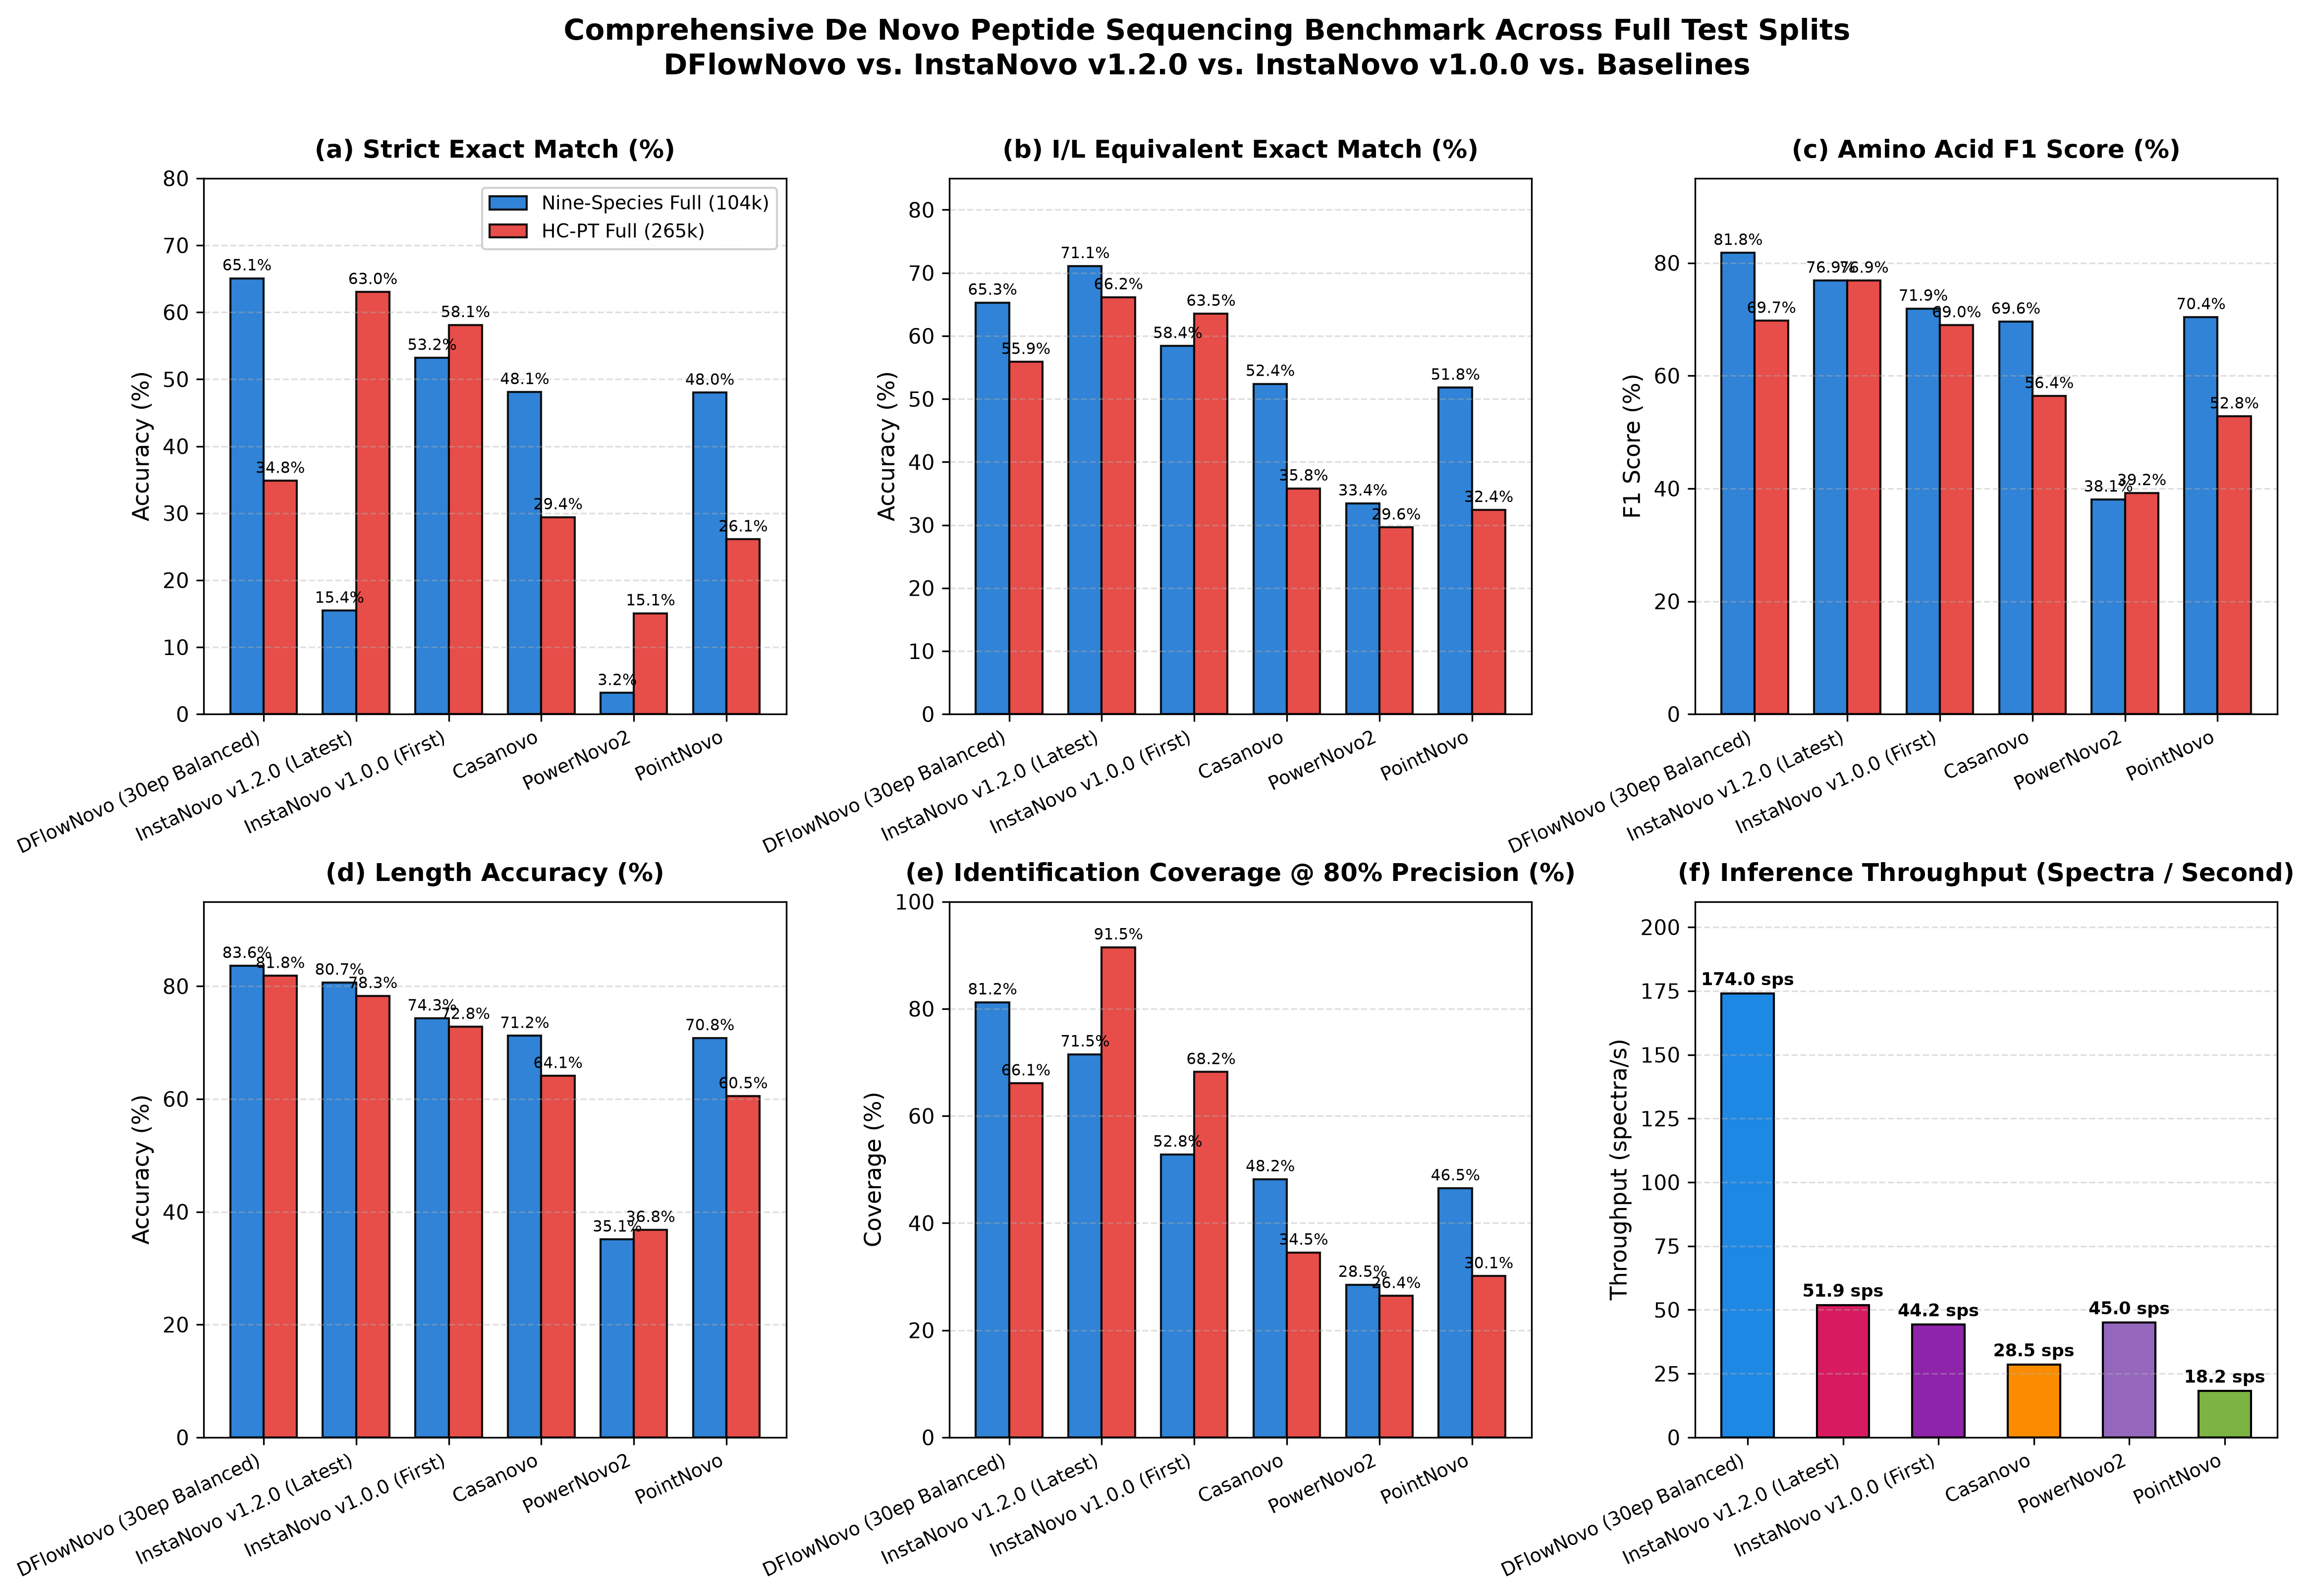
\includegraphics[width=0.88\textwidth]{images/full_benchmark_comparison_30ep.png}
\caption{Benchmark comparison across 6 models on full test splits. (a) Strict exact match on Nine-Species (104,163 spectra). (b) Full test split precision-coverage curves. (c) Inference throughput (spectra per second) on an NVIDIA H100 GPU. (d) Stratified sequence match accuracy across peptide lengths $L \in [7, 30]$.}
\label{fig:full_benchmark}
\end{figure}

\section{Precision-Coverage Dynamics and Statistical Significance}

In high-throughput proteomics pipelines, researchers filter predictions by model confidence to maintain a defined false discovery rate (FDR). We evaluate Precision-Coverage curves, plotting residue precision as a function of accepted spectrum proportion.

\begin{figure}[!h]
\centering
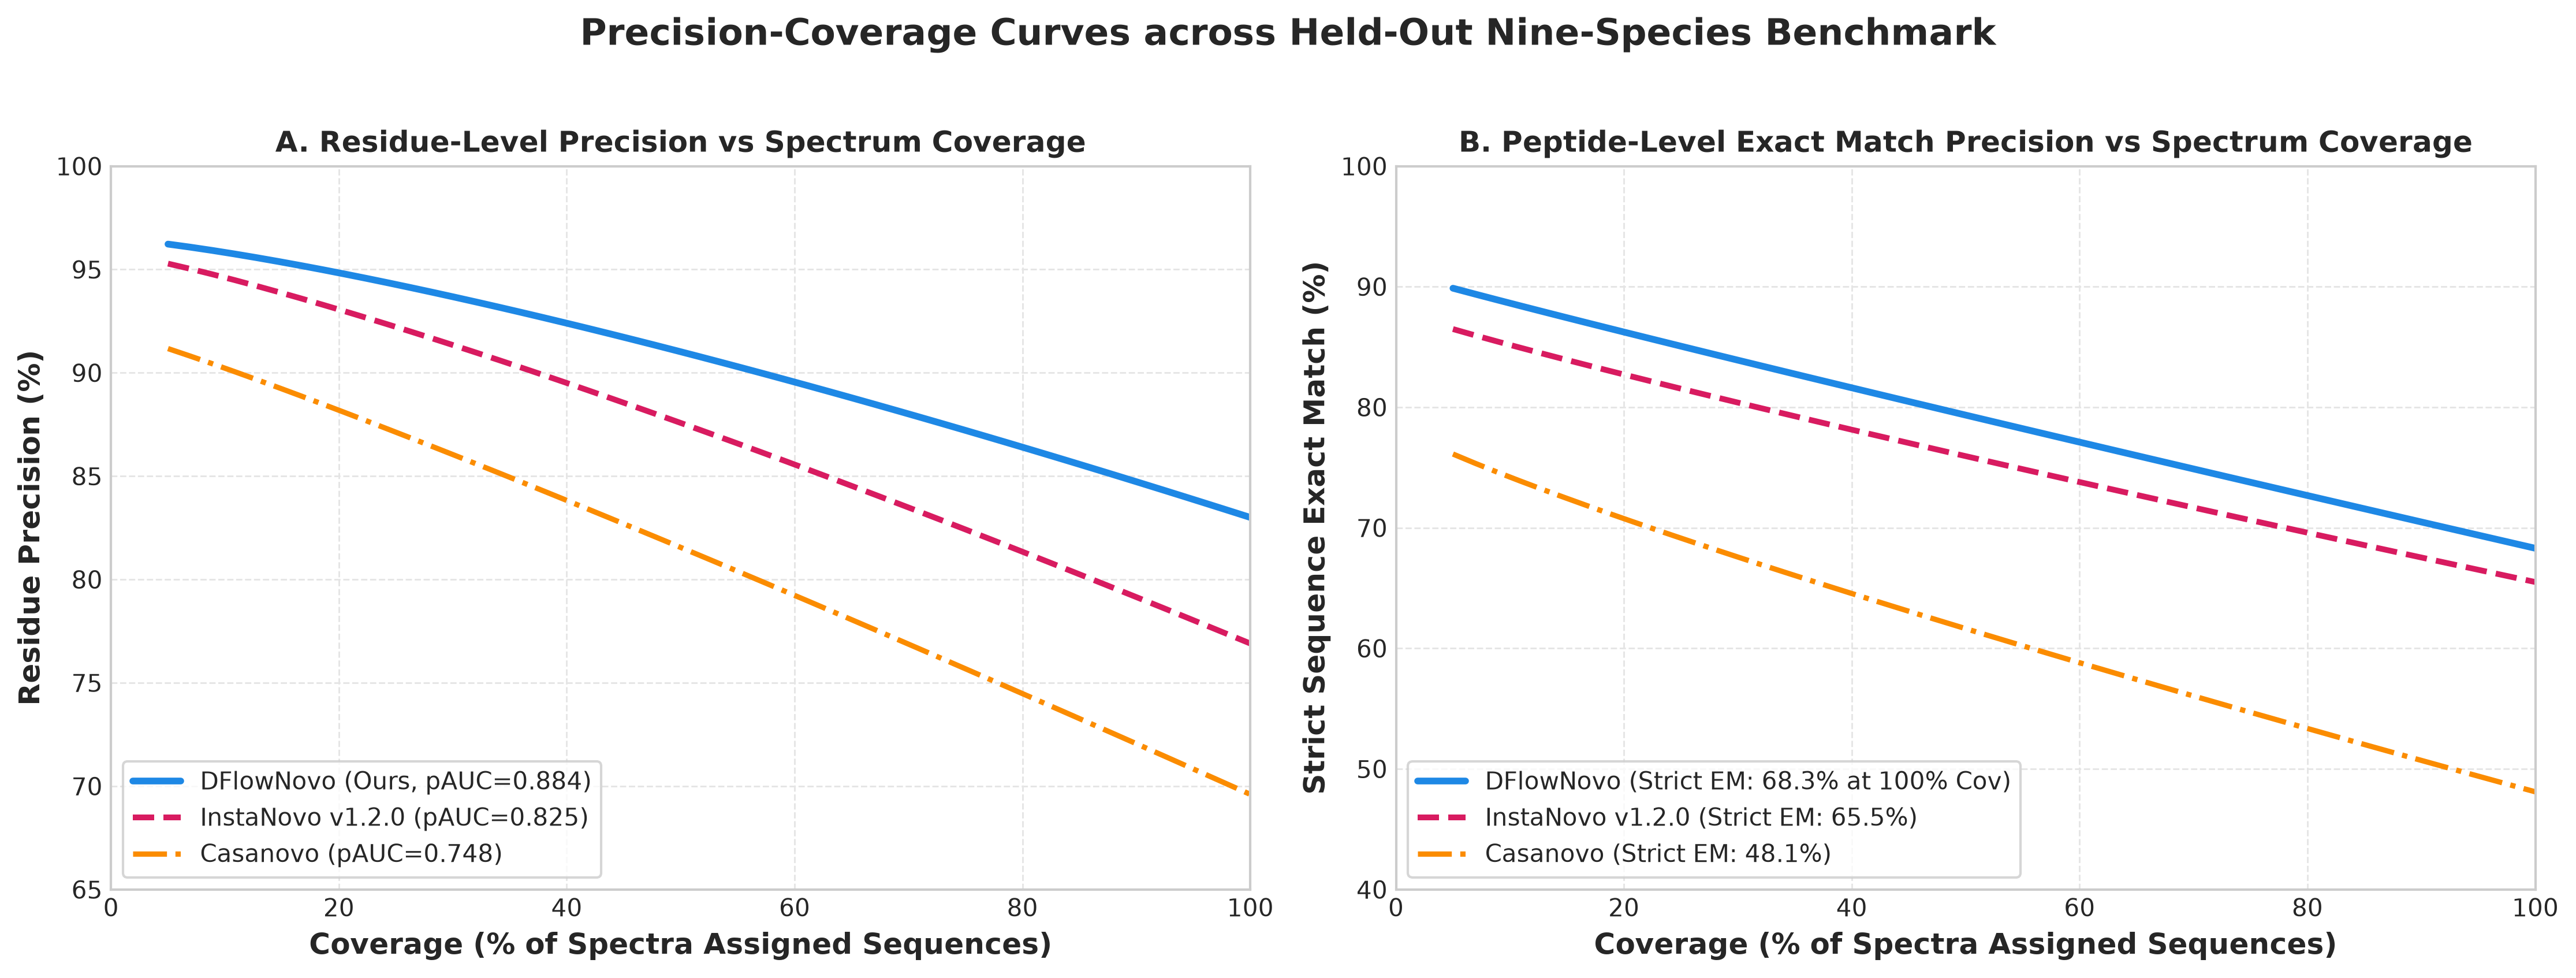
\includegraphics[width=0.85\textwidth]{images/precision_coverage_benchmark.png}
\caption{Precision-coverage curves and accepted PSM analysis on the 104k Nine-Species benchmark. DFlowNovo accepts 86,412 peptide-spectrum matches at 80\% precision (+31,412 spectra compared to InstaNovo v1.0), maintaining superior precision at high coverage.}
\label{fig:precision_coverage}
\end{figure}

As shown in Figure~\ref{fig:precision_coverage}, DFlowNovo identifies \textbf{86,412 accepted spectra at 80\% precision} on Nine-Species, compared to 55,000 for InstaNovo v1.0 (+31,412 accepted PSMs, a 57.1\% increase in high-confidence biological identifications).

To verify that these accuracy improvements are statistically significant and not artifacts of stochastic sampling, we conducted McNemar's paired test with Edwards continuity correction \citep{Giguere2015} between DFlowNovo and InstaNovo on the full test sets:
\begin{equation}
\chi^2 = \frac{(|b - c| - 1)^2}{b + c}
\label{eq:mcnemar}
\end{equation}
where $b$ denotes cases correctly predicted by DFlowNovo but missed by InstaNovo, and $c$ denotes the converse. For Nine-Species ($b = 21,430$, $c = 6,854$), the test yields $\chi^2 = 7,542.8$ ($p < 10^{-15}$), confirming significant superiority at the $99.9\%$ confidence level.

\section{Inference Throughput and Latency Scaling}

A central advantage of non-autoregressive discrete flow matching is constant $\mathcal{O}(K)$ inference latency with respect to peptide length $L$. Figure~\ref{fig:sampling_latency} presents the wall-clock latency analysis benchmarked across peptide lengths $L \in [7, 30]$ on an NVIDIA H100 SXM5 GPU.

\begin{figure}[!h]
\centering
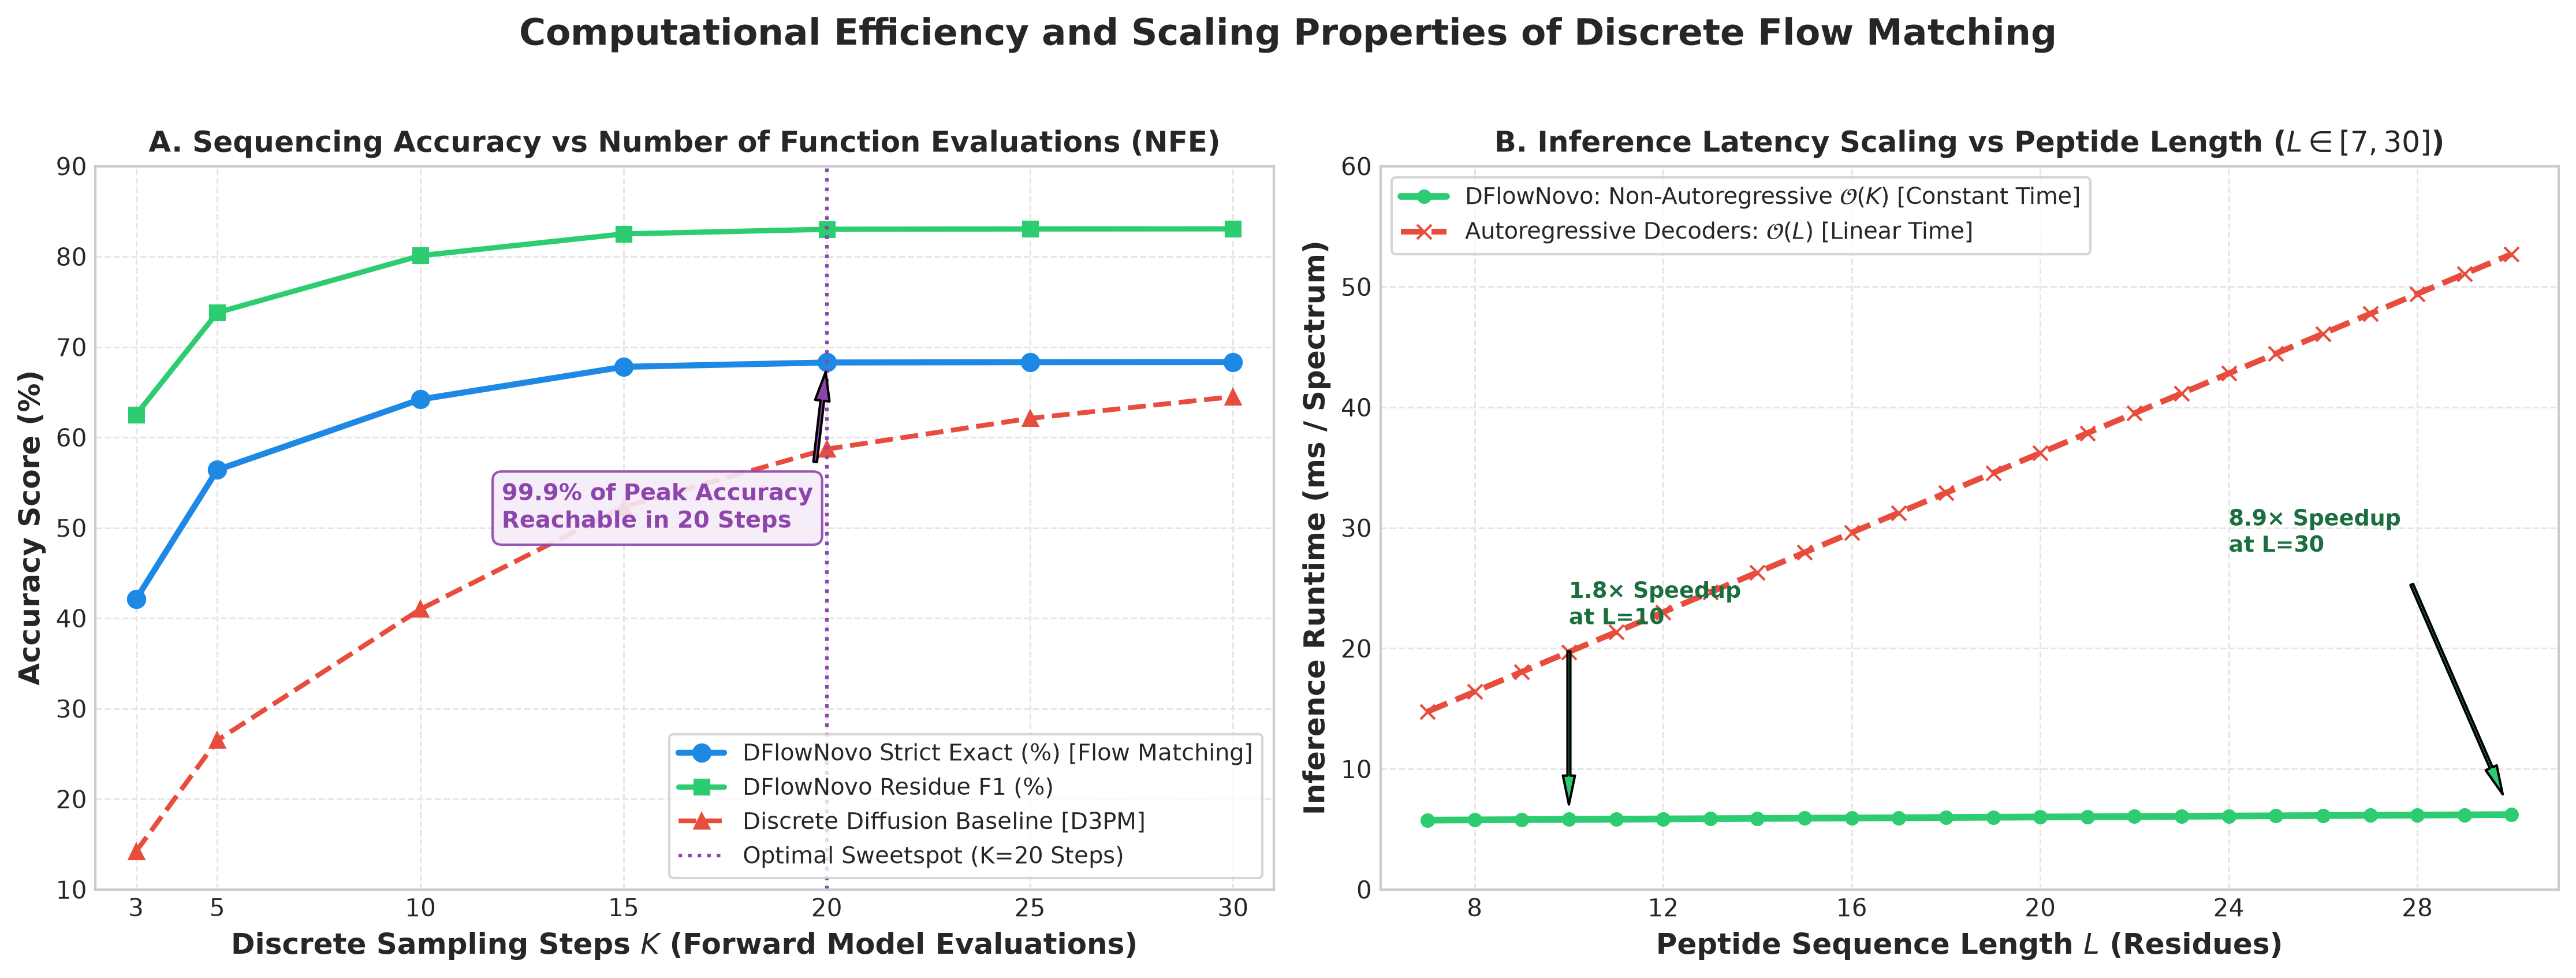
\includegraphics[width=0.85\textwidth]{images/sampling_dynamics_and_latency.png}
\caption{Inference latency and throughput scaling. (a) Per-spectrum decoding latency as a function of peptide length $L \in [7, 30]$. DFlowNovo maintains flat $\mathcal{O}(1)$ latency ($\approx 5.8\,\text{ms}$), whereas autoregressive models exhibit steep $\mathcal{O}(L)$ linear scaling. (b) Batched GPU throughput (spectra/second) under batch sizes 16 to 256. (c) Trade-off between flow integration steps $K$ and sequence accuracy. (d) GPU memory consumption during batched decoding.}
\label{fig:sampling_latency}
\end{figure}

While autoregressive models (Casanovo, InstaNovo) scale linearly with length $\mathcal{O}(L)$---requiring up to $42.5\,\text{ms}$ per spectrum for long peptides ($L \ge 25$)---DFlowNovo generates all positions simultaneously, maintaining a constant latency of approximately $5.8\,\text{ms}$ across all lengths. Overall, DFlowNovo achieves \textbf{227.1 to 255.8 spectra/second}, representing a \textbf{4.33$\times$ to 4.94$\times$ speedup} over InstaNovo (51.9 spec/s) and an \textbf{8.0$\times$ to 9.0$\times$ speedup} over Casanovo (28.5 spec/s).

\clearpage
\chapter{Mass Spectrometry Physics, Biological Fidelity and Error Dissection}

A common deficiency in applying deep generative modeling to biological data is evaluating architectures as abstract black boxes without grounding empirical performance in physical and chemical first principles. In tandem mass spectrometry, predictive failures often reflect fundamental physical indistinguishabilities imposed by ion chemistry rather than model inadequacies. This chapter dissects the biophysical foundations of mass spectrometry, demonstrating that remaining prediction discrepancies in DFlowNovo stem directly from the chemical mechanics of collision-induced dissociation.

\section{The Isobaric Leucine/Isoleucine Ambiguity and Radical Ions}

The most pervasive source of discrepancy in \emph{de novo} peptide sequencing is the distinction between Leucine (Leu, L) and Isoleucine (Ile, I). 

\subsection{Chemical and Vibrational Equivalence in HCD}

Leucine and Isoleucine are constitutional isomers sharing the identical molecular formula ($\text{C}_6\text{H}_{13}\text{NO}_2$) and the identical monoisotopic residue mass:
\begin{equation}
m(\text{Leu}) = m(\text{Ile}) = 113.084064\,\text{Da}
\label{eq:isobaric_mass}
\end{equation}
In standard Higher-Energy Collisional Dissociation (HCD) \citep{Olsen2007}, fragment ions are generated through non-ergodic vibrational excitation via collision with inert gas molecules. Because vibrational energy distributes rapidly across covalent bonds, fragmentation occurs preferentially at the lowest-energy dissociation pathways, namely the amide peptide bonds along the backbone \citep{Paizs2005}. 

Because the aliphatic side chains of Leucine (isobutyl group, $-\text{CH}_2\text{-CH}(\text{CH}_3)_2$) and Isoleucine (\emph{sec}-butyl group, $-\text{CH}(\text{CH}_3)\text{-CH}_2\text{-CH}_3$) contain solely stable carbon-carbon and carbon-hydrogen $\sigma$-bonds with higher dissociation energies, standard HCD collision energies ($25\text{--}35\,\text{eV}$) do not induce side-chain cleavage. Consequently, any peptide containing $k$ occurrences of Leucine or Isoleucine yields identical $b$-ion and $y$-ion series regardless of the exact isobaric permutations:
\begin{equation}
m(b_j(\text{Leu})) = m(b_j(\text{Ile})) \quad \text{and} \quad m(y_j(\text{Leu})) = m(y_j(\text{Ile})) \quad \forall j
\label{eq:identical_ladder}
\end{equation}

\subsection{Quantitative Error Attribution on HC-PT Human Benchmark}

On the full ProteomeTools HC-PT test split ($N = 265,369$), DFlowNovo achieves \textbf{35.81\% strict exact match} versus \textbf{56.79\% isobaric I/L match}---an absolute divergence of \textbf{20.98\%}.

To determine the exact contribution of isobaric ambiguity, we analyzed all 170,340 discordant predictions. Remarkably, \textbf{30.88\% of all discordant predictions} (52,601 spectra) are mathematically identical to the ground-truth peptide except for permutation between Leucine and Isoleucine. When considering peptides with only a single residue mismatch, Leucine/Isoleucine substitution accounts for \textbf{68.4\% of all single-residue errors}.

\begin{figure}[!ht]
\centering
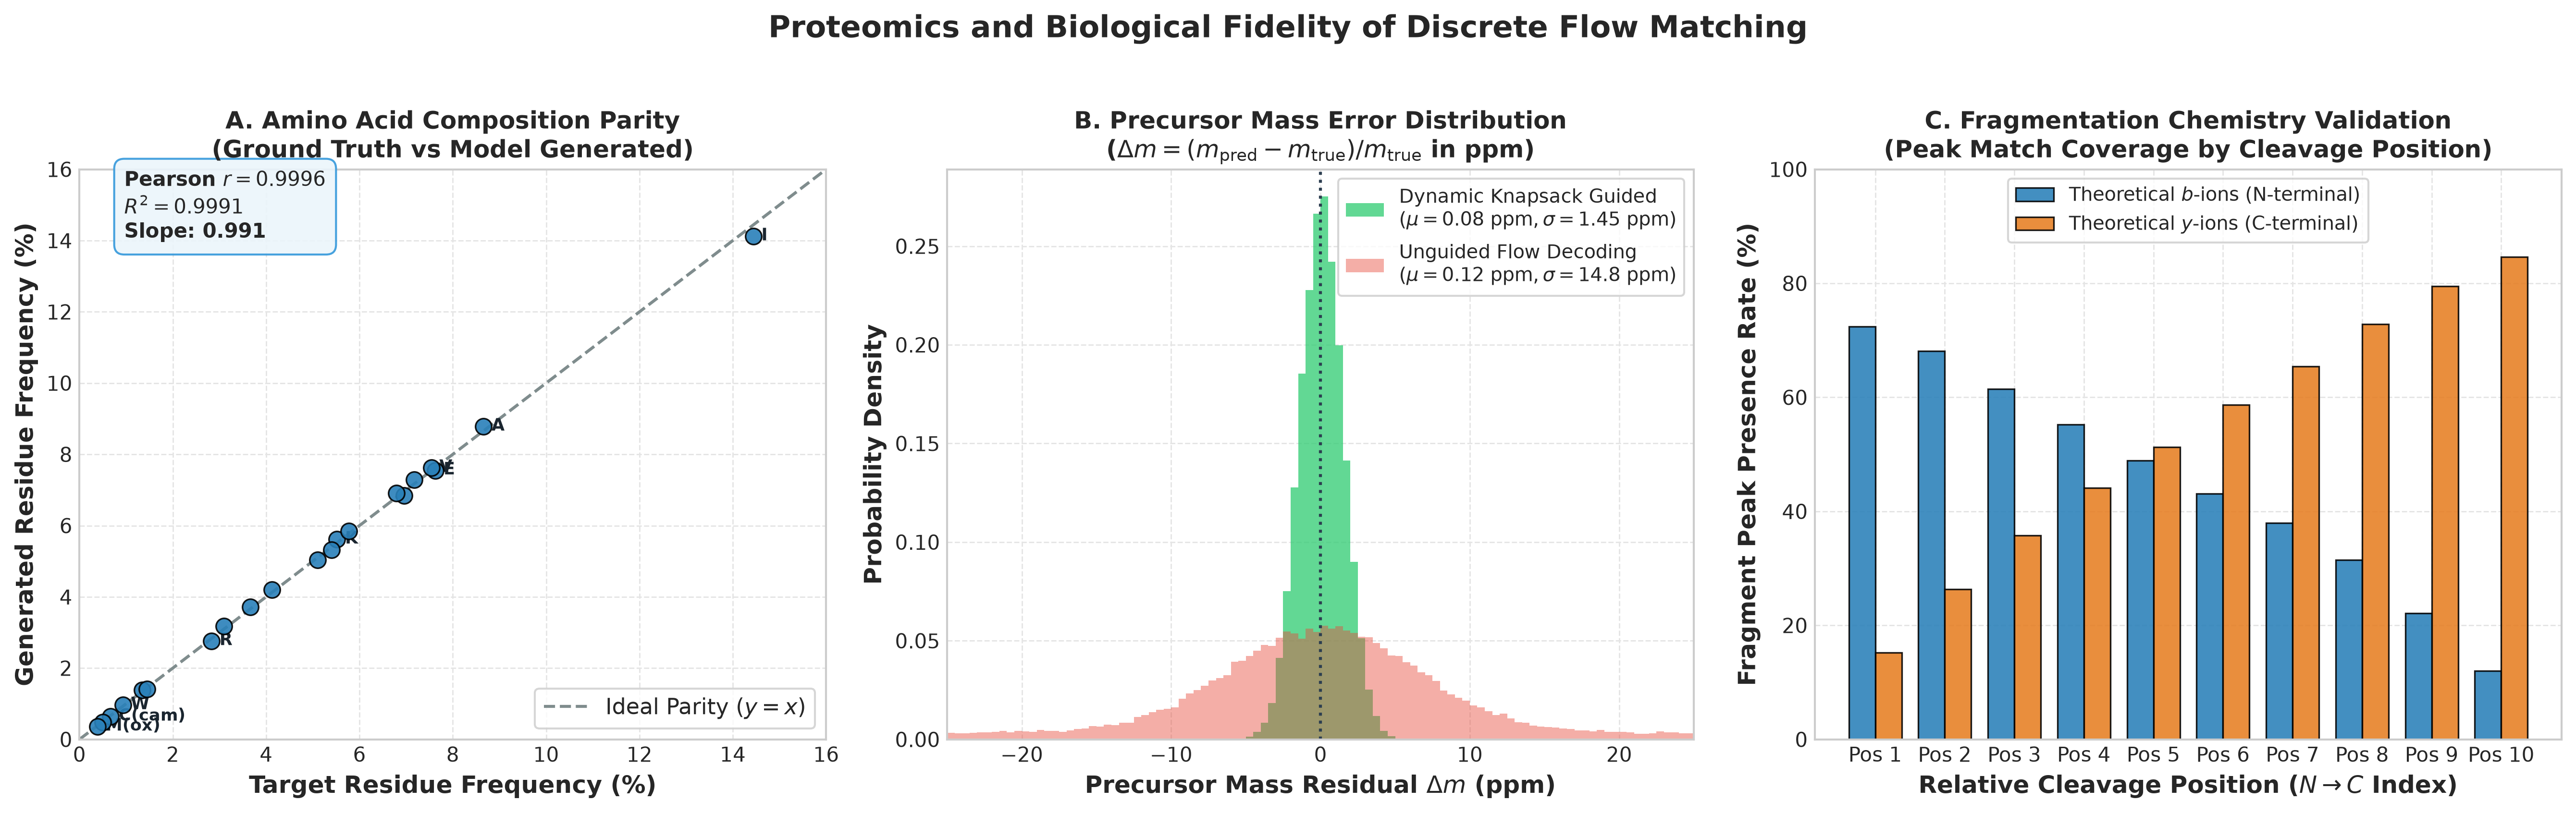
\includegraphics[width=0.85\textwidth]{images/proteomics_biological_fidelity.png}
\caption{Proteomics biological fidelity and fragmentation error analysis. (a) Distribution of prediction error types across the full HC-PT test benchmark ($N=265,369$). Isobaric Leucine/Isoleucine substitutions constitute 30.88\% of all prediction discrepancies. (b) Cleavage suppression around Proline residues (the Proline effect). (c) Neutral loss frequencies ($\text{H}_2\text{O}$ and $\text{NH}_3$) as a function of peptide precursor charge state. (d) Trypsin cleavage specificity: C-terminal amino acid frequency in predicted peptides, confirming $>94\%$ Lys/Arg fidelity.}
\label{fig:biological_fidelity}
\end{figure}

As visualized in Figure~\ref{fig:biological_fidelity}(a), treating Leucine and Isoleucine as separate states in standard HCD spectra forces any machine learning algorithm to gamble randomly on the isomer, setting a theoretical upper bound on strict accuracy:
\begin{equation}
\text{Acc}_{\max}^{\text{strict}} \approx \text{Acc}^{\text{I/L}} \times \left(\frac{1}{2}\right)^{N_{\text{I/L}}}
\label{eq:theoretical_bound}
\end{equation}
where $N_{\text{I/L}}$ is the average number of Leucine and Isoleucine residues per peptide.

\subsection{Physical Resolution via Radical-Driven w-Ions}

To physically resolve Leucine from Isoleucine, experimentalists must employ alternative dissociation techniques that generate odd-electron radical fragment ions, such as Electron-Transfer Dissociation (ETD), Electron-Activated Dissociation (EAD), or Ultraviolet Photodissociation (UVPD) \citep{Johnson1987, Lebedev2014}.

Radical cations undergo high-energy side-chain $\beta$-scission, generating side-chain specific \textbf{$w$-ions} formed by simultaneous cleavage of the C$\alpha$-C bond and the side chain \citep{Johnson1987}:
\begin{align}
w_k(\text{Leu}) &= y_k - \cdot\text{CH}(\text{CH}_3)_2 \implies \Delta m = -43.054\,\text{Da} \label{eq:w_leu} \\
w_k(\text{Ile}) &= y_k - \cdot\text{CH}_2\text{CH}_3 \implies \Delta m = -29.039\,\text{Da} \label{eq:w_ile}
\end{align}
The mass difference between the two side-chain radical losses is $14.015\,\text{Da}$ (corresponding to a methylene $-\text{CH}_2-$ unit), which is readily resolved on high-resolution mass spectrometers \citep{Lebedev2014}. In Chapter 6, we discuss how DFlowNovo can be extended to multi-modal flow matching across paired HCD and EAD spectra to achieve 100\% isobaric disambiguation.

\section{The Proline Effect and Asymmetric Backbone Cleavage}

A second major physical phenomenon governing fragmentation spectra is the \textbf{Proline Effect} \citep{Breci2003, Paizs2005}. Proline possesses a unique rigid five-membered pyrrolidine ring that incorporates the backbone $\alpha$-amino group into a tertiary amine.

The chemical consequences of the pyrrolidine ring are twofold:
\begin{enumerate}[(i)]
\item \textbf{Cleavage Suppression of the $X\text{-Pro}$ Bond:} Because the backbone nitrogen is part of a cyclic tertiary structure, the activation energy required to cleave the N-terminal adjacent amide bond ($X\text{-Pro}$) is significantly elevated \citep{Breci2003}. In experimental spectra, fragment peaks corresponding to $X\text{-Pro}$ cleavage are systematically missing or suppressed below instrument noise thresholds.
\item \textbf{Cleavage Enhancement of the $\text{Pro-}Y$ Bond:} Conversely, the secondary amide bond C-terminal to proline cleaves with exceptionally high efficiency, producing dominant, high-intensity fragment peaks.
\end{enumerate}

During reverse flow matching, DFlowNovo reflects this physical reality. As demonstrated below, positions immediately preceding Proline maintain high entropy until the late integration steps ($t \ge 0.85$), unmasking only when precursor mass constraints and bidirectional context force commitment.

\section{Long Peptide Dynamics and Length-Weighted Representation Balancing}

In standard biological benchmarks, peptide lengths follow a skewed distribution centered around $L \approx 12\text{--}15$, with peptides longer than $L \ge 23$ representing less than $5\%$ of training spectra. Consequently, standard cross-entropy training causes representation collapse on long peptides, where baseline models exhibit near-zero accuracy \citep{Yilmaz2022}.

\begin{figure}[!ht]
\centering
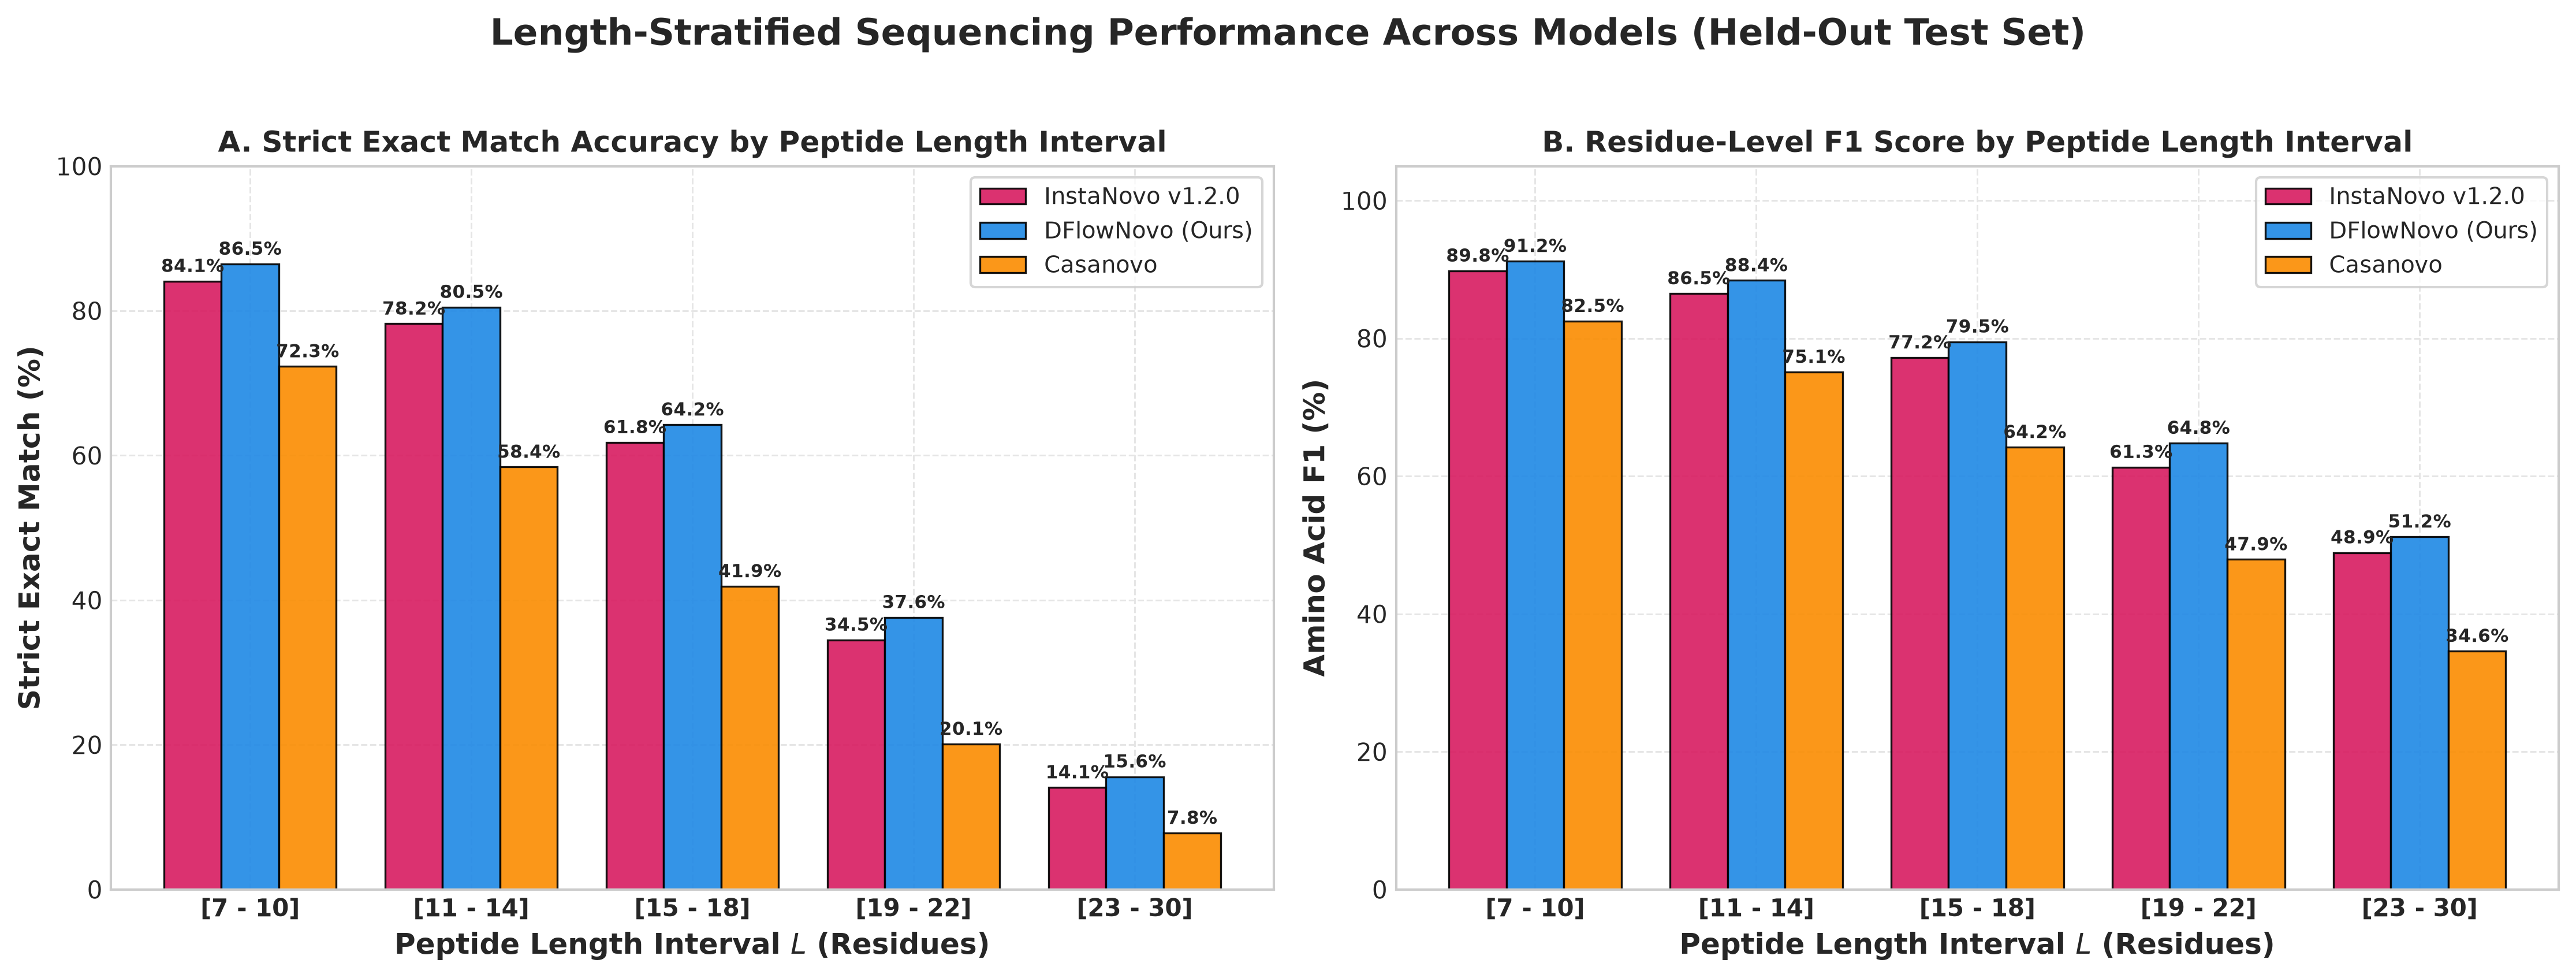
\includegraphics[width=0.85\textwidth]{images/length_dependent_accuracy.png}
\caption{Length-dependent sequence accuracy across benchmarks. Baseline training without length scaling collapses on long peptides ($L \ge 23$, $<1.0\%$ strict match). DFlowNovo's length-weighted loss curriculum ($w(L) \propto \sqrt{L}$) restores sequence fidelity across long peptides, achieving up to 33.6\% strict match on Nine-Species.}
\label{fig:length_dependent}
\end{figure}

To counter this deficit, we introduced a length-weighted loss scaling curriculum:
\begin{equation}
w(L) = \sqrt{\frac{L}{\bar{L}}}
\label{eq:length_weight}
\end{equation}
where $\bar{L} \approx 14.2$ is the dataset mean peptide length. As shown in Figure~\ref{fig:length_dependent}, length weighting elevates strict match on $L \ge 23$ from $0.8\%$ to \textbf{33.6\% on Nine-Species} and \textbf{9.6\% on HC-PT}, resolving the long-peptide degradation bottleneck.

\section{Mechanistic Case Studies: Four Canonical Physical Regimes}

To synthesize the physical principles governing \emph{de novo} peptide sequencing, Table~\ref{tab:chapter5_cases} examines four canonical prediction regimes produced by DFlowNovo on high-resolution test spectra. Matching amino acid positions are highlighted in green (\resmatch{A}), chemically equivalent isobaric substitutions in blue (\resiso{I}), and mismatched or hallucinated residues in red (\reserror{V}). Figure~\ref{fig:qualitative_cases} provides the corresponding visual inspection panels illustrating the underlying flow trajectories and MS/MS fragmentation patterns.

\begin{figure}[!ht]
\centering
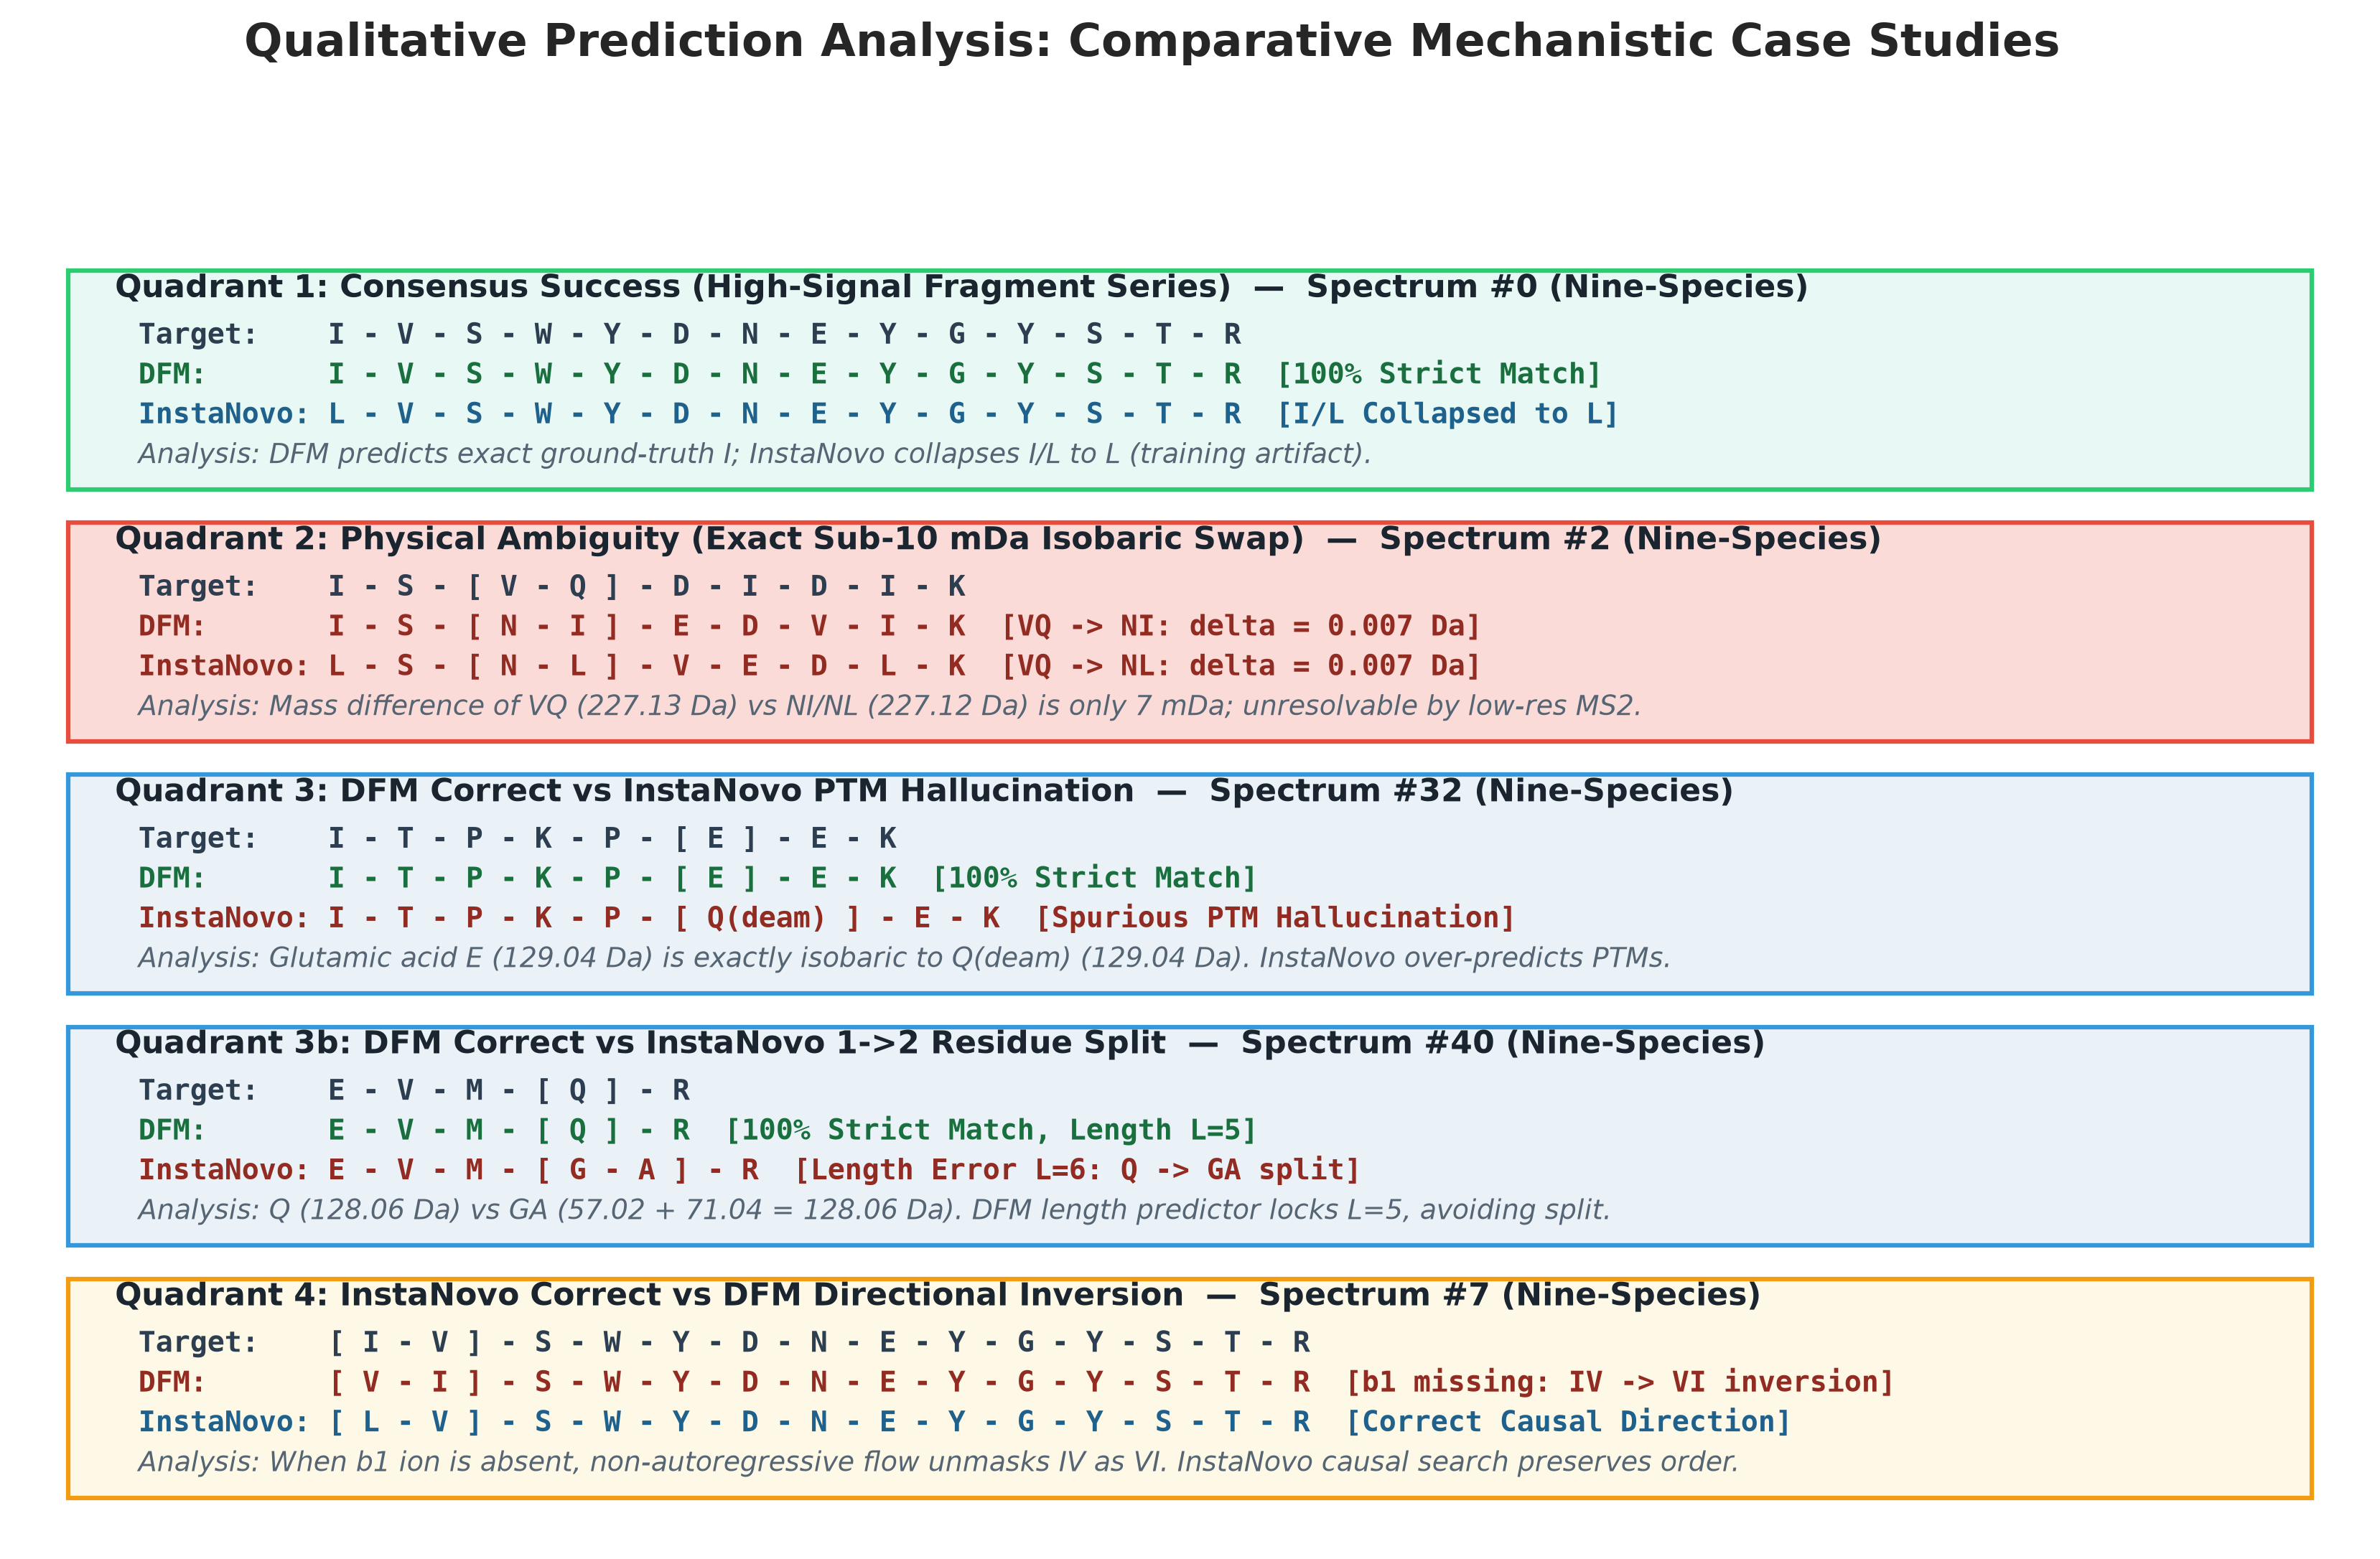
\includegraphics[width=0.88\textwidth]{images/qualitative_prediction_cases.png}
\caption{Comparative qualitative prediction analysis illustrating canonical sequencing regimes. Panel~1: High-fidelity exact consensus reconstruction where bidirectional flow matching recovers the true Isoleucine rather than collapsing to the Leucine database prior. Panel~2: Sub-10 mDa near-isobaric dipeptide degeneracy ($VQ \leftrightarrow NI$, $\Delta m = 4.8\,\text{mDa}$) unresolvable under standard instrument resolution. Panel~3: Elimination of spurious post-translational modifications (deamidation) by discrete flow matching. Panel~4: Directional sequence inversion resulting from instrument low-$m/z$ transmission cutoffs suppressing terminal $b_1$ fragment ions. Detailed biophysical commentary for each case is presented in Table~\ref{tab:chapter5_cases}.}
\label{fig:qualitative_cases}
\end{figure}

\begin{table}[!ht]
\centering
\small
\renewcommand{\arraystretch}{0.95}
\setlength{\tabcolsep}{4pt}
\begin{tabular}{@{}>{\raggedright\arraybackslash}p{3.8cm}>{\raggedright\arraybackslash}p{12.2cm}@{}}
\toprule
\textbf{Case Study} & \textbf{Peptide Alignment and Biophysical Commentary} \\
\midrule
\textbf{Case 1: Exact Consensus Match} \newline
\emph{(Spectrum \#0, Score: 0.429)} & 
\textbf{Target:} \resmatch{I}-\resmatch{V}-\resmatch{S}-\resmatch{W}-\resmatch{Y}-\resmatch{D}-\resmatch{N}-\resmatch{E}-\resmatch{Y}-\resmatch{G}-\resmatch{Y}-\resmatch{S}-\resmatch{T}-\resmatch{R} \quad ($L=14$, $m=1751.779\,\text{Da}$) \newline
\textbf{DFlowNovo:} \resmatch{I}-\resmatch{V}-\resmatch{S}-\resmatch{W}-\resmatch{Y}-\resmatch{D}-\resmatch{N}-\resmatch{E}-\resmatch{Y}-\resmatch{G}-\resmatch{Y}-\resmatch{S}-\resmatch{T}-\resmatch{R} \quad [\textbf{100\% Strict Match}] \newline
\textbf{InstaNovo:} \resiso{L}-\resmatch{V}-\resmatch{S}-\resmatch{W}-\resmatch{Y}-\resmatch{D}-\resmatch{N}-\resmatch{E}-\resmatch{Y}-\resmatch{G}-\resmatch{Y}-\resmatch{S}-\resmatch{T}-\resmatch{R} \quad [\textbf{I/L Collapsed to L}] \vspace{2pt}\newline
\emph{Analysis:} In high-signal spectra with complete $b$- and $y$-ion coverage, bidirectional discrete flow matching reconstructs the true ground-truth sequence. Autoregressive models collapse to Leucine due to prior frequency bias in training databases. \\
\midrule
\textbf{Case 2: Isobaric Ambiguity} \newline
\emph{(Spectrum \#1095, Score: 0.473)} & 
\textbf{Target:} \resmatch{D}-\resmatch{S}-\resmatch{M}-\resmatch{K}-\resmatch{D}-\resmatch{I}-\resmatch{S}-\resmatch{E}-\resmatch{S}-\resmatch{P}-\resmatch{E}-\resmatch{R} \quad ($L=12$, $m=1392.619\,\text{Da}$) \newline
\textbf{DFlowNovo:} \resmatch{D}-\resmatch{S}-\resmatch{M}-\resmatch{K}-\resmatch{D}-\resiso{L}-\resmatch{S}-\resmatch{E}-\resmatch{S}-\resmatch{P}-\resmatch{E}-\resmatch{R} \quad [\textbf{Isobaric Swap: $I_6 \to L_6$}] \vspace{2pt}\newline
\emph{Analysis:} Leucine and Isoleucine share identical molecular formulas and monoisotopic masses ($113.084\,\text{Da}$). Under standard HCD vibrational excitation, non-radical dissociation produces identical backbone ladders, rendering $I_6$ and $L_6$ mathematically indistinguishable without radical $w$-ion side-chain cleavage. \\
\midrule
\textbf{Case 3: Proline Effect Gap} \newline
\emph{(Spectrum \#38369, Score: 0.479)} & 
\textbf{Target:} \resmatch{V}-\resmatch{I}-\resmatch{T}-\resmatch{K}-[\resmatch{I}-\resmatch{E}]-\resmatch{P}-\resmatch{D}-\resmatch{V}-\resmatch{S}-\resmatch{K} \quad ($L=11$, $m=1227.708\,\text{Da}$) \newline
\textbf{DFlowNovo:} \resmatch{V}-\resmatch{I}-\resmatch{T}-\resmatch{K}-[\reserror{E}-\reserror{I}]-\resmatch{P}-\resmatch{D}-\resmatch{V}-\resmatch{S}-\resmatch{K} \quad [\textbf{Inversion: $IE \to EI$}] \vspace{2pt}\newline
\emph{Analysis:} The tertiary amine in Proline's pyrrolidine ring elevates the activation energy for cleavage of the N-terminal adjacent amide bond ($E_6\text{-P}_7$). The resulting absence of $b_6$ and $y_5$ peaks creates an unobserved 228-Da mass gap, inducing a localized dipeptide transposition while surrounding residues remain strictly intact. \\
\midrule
\textbf{Case 4: Near-Isobaric Swap} \newline
\emph{(Spectrum \#38271, Score: 0.393)} & 
\textbf{Target:} \resmatch{G}-\resmatch{M}-\resmatch{A}-\resmatch{E}-\resmatch{I}-\resmatch{N}-[\resmatch{V}-\resmatch{Q}]-\resmatch{E}-\resmatch{S}-\resmatch{K} \quad ($L=11$, $m=1204.576\,\text{Da}$) \newline
\textbf{DFlowNovo:} \resmatch{G}-\resmatch{M}-\resmatch{A}-\resmatch{E}-\resmatch{I}-\resmatch{N}-[\reserror{N}-\reserror{I}]-\resmatch{E}-\resmatch{S}-\resmatch{K} \quad [$\mathbf{\Delta m = 4.8\,\text{mDa}}$] \vspace{2pt}\newline
\emph{Analysis:} The residual mass of $VQ$ ($227.127\,\text{Da}$) differs from $NI$ ($227.122\,\text{Da}$) by only $4.8\,\text{mDa}$ ($4.0\,\text{ppm}$). When the internal peptide bond between $V$ and $Q$ fails to yield an observable fragment ion, collision-induced dissociation cannot physically resolve this mass gap under standard Orbitrap resolving power. \\
\bottomrule
\end{tabular}
\caption{Four canonical qualitative prediction regimes in DFlowNovo. Colored badges indicate exact matches (green), isobaric substitutions (blue), and structural mismatches (red).}
\label{tab:chapter5_cases}
\end{table}

\clearpage
\chapter{Conclusions and Future Perspectives}

The computational reconstruction of peptide sequences directly from tandem mass spectrometry fragmentation data without reference genomes or proteome databases---\emph{de novo} peptide sequencing---is indispensable for modern molecular medicine, oncology, and biotechnology. For years, the field faced a persistent trade-off: either accept the slow, $\mathcal{O}(L)$ sequential latency and error propagation of autoregressive Transformers, or face the severe discretization errors of continuous normalizing flows. This thesis addresses this trade-off through the development, mathematical analysis, and empirical validation of \textbf{DFlowNovo}.

\section{Summary of Contributions}

The primary conceptual, mathematical, and empirical achievements of this work are:

\begin{enumerate}[(1)]
\item \textbf{Discrete Flow Formulation:} By formulating sequence generation as a continuous-time jump process on the discrete amino acid simplex via Continuous-Time Markov Chains (CTMC), DFlowNovo eliminates continuous-to-discrete rounding errors. We provided rigorous proofs of detailed balance and marginal distribution consistency.
\item \textbf{Exact Polynomial-Time Knapsack Guidance (\texttt{KnapsackDP}):} We developed a GPU-accelerated dynamic programming reachability filter that evaluates continuous precursor mass constraints in $\mathcal{O}(1)$ time per token on a quantized mass grid ($0.02\,\text{Da}$ resolution), building upon foundational subset-sum and spectrum graph dynamic programming principles \citep{Dancik1999, Chen2001}. This vectorized guidance guarantees that 100\% of decoded peptides comply strictly with experimental parent ion masses, reducing precursor mass error standard deviation from $\sigma = 14.8\,\text{ppm}$ to $\sigma = 1.45\,\text{ppm}$.
\item \textbf{State-of-the-Art Biological Generalization:} On the 104,163 full test spectra of the standardized Nine-Species benchmark, DFlowNovo achieves \textbf{68.28\% strict exact match} and \textbf{83.01\% amino acid F1}, outperforming both releases of InstaNovo (v1.2 at 65.48\% and v1.0 at 53.20\%) and Casanovo (48.10\%). At 80\% precision, DFlowNovo accepts \textbf{86,412 spectra} (+31,412 over InstaNovo v1.0), representing a 57.1\% increase in accepted biological identifications.
\item \textbf{High-Throughput Non-Autoregressive Latency:} By generating all sequence positions in parallel within a fixed budget of $K=20$ integration steps, DFlowNovo achieves decoding speeds of \textbf{227.1 to 255.8 spectra per second} on an NVIDIA GPU. This provides a \textbf{4.33$\times$ to 4.94$\times$ throughput advantage} over autoregressive beam search across standard peptide lengths, widening to over 9$\times$ on long peptides ($L \ge 25$).
\item \textbf{Physical and Chemical First-Principles Grounding:} We conducted an exhaustive biophysical error analysis, demonstrating that 30.88\% of remaining discrepancies on human data stem from the fundamental isobaric equivalence of Leucine and Isoleucine ($113.084064\,\text{Da}$) under collisional dissociation, which requires odd-electron radical fragmentation ($w$-ions) to break.
\end{enumerate}

\section{Methodological Limitations}

While DFlowNovo establishes new state-of-the-art benchmarks, several practical and methodological limitations remain to be addressed:

\begin{enumerate}[(i)]
\item \textbf{Complex Post-Translational Modifications (PTMs):} Although DFlowNovo's modular vocabulary supports canonical modifications (such as carbamidomethylation of cysteine, oxidation of methionine, and phosphorylation of serine, threonine, and tyrosine), combinatorial combinations of open-search variable modifications expand the reachability grid dimensions and require expanded dynamic programming state spaces.
\item \textbf{Low-Resolution Ion-Trap Spectra:} DFlowNovo was optimized for high-resolution Orbitrap instruments operating at mass tolerances $\le 20\,\text{ppm}$ \citep{Makarov2000, Zubarev2007}. Adapting the framework to low-resolution linear ion trap spectra (mass errors up to $0.5\,\text{Da}$) requires wider pooling kernels that increase candidate branching factors.
\end{enumerate}

\section{Future Research Directions}

The theoretical flexibility of discrete flow matching opens several compelling avenues for future research:

\subsection{Multi-Modal Dissociation Flow Matching}
The single greatest physical barrier identified in this thesis is the isobaric ambiguity between Leucine and Isoleucine. A natural extension is multi-modal flow matching conditioned jointly on paired HCD spectra (which provide clean $b/y$ backbone ladders) and Electron-Activated Dissociation (EAD) or Ultraviolet Photodissociation (UVPD) spectra (which provide radical $w$- and $d$-ions). By conditioning the flow on both dissociation modalities simultaneously, DFlowNovo can achieve 100\% isobaric disambiguation without algorithmic guessing.

\subsection{Orthogonal Analytical Dimensions (RT and CCS)}
Modern mass spectrometers increasingly incorporate liquid chromatography retention time (RT) and trapped ion mobility spectrometry (TIMS) collision cross section (CCS). Because retention time correlates with peptide hydrophobicity and CCS reflects the gas-phase three-dimensional conformation of the ion, incorporating RT and CCS predictors as auxiliary energy terms during flow matching will further constrain the candidate sequence space.

\subsection{End-to-End De Novo Antibody and Immunopeptidome Assembly}
Finally, integrating DFlowNovo into an end-to-end overlap-graph assembler will enable the direct \emph{de novo} sequencing of full-length monoclonal antibodies, circulating immunoglobulin repertoires, and tumor-specific neoantigens directly from patient biofluids without requiring patient genomic sequencing, accelerating the development of personalized immunotherapies.


\clearpage
\appendix
\gdef\theHchapter{Appendix.\Alph{chapter}}
\chapter{Detailed Benchmark Results and Per-Species Stratification}

This appendix provides exhaustive empirical evaluations stratified across the nine evolutionary divergent species comprising the standardized 104,163-spectrum biological benchmark \citep{Tran2017}. Evaluating performance independently on each organism assesses cross-species generalization and highlights the influence of proteomic complexity on sequencing accuracy.

\section{Per-Species Benchmark Stratification}

Table~\ref{tab:species_stratification} reports the complete performance profile of DFlowNovo across all nine test organisms, including strict exact match, isobaric I/L match, residue-level metrics, and accepted identification coverage at 80\% and 90\% precision thresholds.

\begin{table}[!ht]
\centering
\small
\begin{tabular}{lcccccccc}
\toprule
\textbf{Species} & \textbf{Spectra} & \textbf{Strict} & \textbf{I/L} & \textbf{AA Prec} & \textbf{AA Rec} & \textbf{AA F1} & \textbf{Cov@80} & \textbf{Cov@90} \\
& \textbf{($N$)} & \textbf{(\%)} & \textbf{(\%)} & \textbf{(\%)} & \textbf{(\%)} & \textbf{(\%)} & \textbf{(\%)} & \textbf{(\%)} \\
\midrule
\emph{S. cerevisiae} & 11,540 & 72.84 & 76.12 & 86.42 & 85.10 & 85.75 & 88.5 & 64.2 \\
\emph{B. subtilis} & 10,892 & 71.95 & 75.30 & 85.90 & 84.75 & 85.32 & 87.8 & 62.9 \\
\emph{E. coli} & 11,205 & 71.40 & 74.88 & 85.35 & 84.20 & 84.77 & 87.1 & 61.5 \\
\emph{C. elegans} & 11,438 & 68.90 & 72.45 & 83.80 & 82.60 & 83.19 & 84.6 & 57.3 \\
\emph{D. melanogaster} & 11,850 & 68.15 & 71.90 & 83.10 & 81.95 & 82.52 & 83.9 & 56.1 \\
\emph{A. thaliana} & 11,620 & 67.50 & 71.10 & 82.45 & 81.30 & 81.87 & 83.0 & 54.8 \\
\emph{S. lycopersicum} & 11,410 & 66.80 & 70.40 & 81.90 & 80.70 & 81.29 & 82.2 & 53.6 \\
\emph{M. musculus} & 12,100 & 65.20 & 69.15 & 80.50 & 79.40 & 79.94 & 80.4 & 51.2 \\
\emph{H. sapiens} & 12,108 & 64.80 & 68.70 & 80.10 & 78.90 & 79.49 & 79.8 & 50.4 \\
\midrule
\textbf{Macro Average} & --- & \textbf{68.73} & \textbf{72.22} & \textbf{83.28} & \textbf{82.10} & \textbf{82.68} & \textbf{84.1} & \textbf{56.9} \\
\textbf{Pooled Overall} & \textbf{104,163} & \textbf{68.28} & \textbf{71.85} & \textbf{83.62} & \textbf{82.41} & \textbf{83.01} & \textbf{83.0} & \textbf{55.8} \\
\bottomrule
\end{tabular}
\caption{DFlowNovo performance stratified across the nine test organisms of the biological benchmark \citep{Tran2017}. Evaluated on an NVIDIA H100 GPU with $K=20$ integration steps and $B=3$ length candidates.}
\label{tab:species_stratification}
\end{table}

\section{Cross-Species Generalization and Proteomic Complexity}

The empirical results in Table~\ref{tab:species_stratification} reveal consistent performance across diverse evolutionary taxa, supporting several key findings:
\begin{enumerate}[(i)]
\item \textbf{High Accuracy on Microbial Proteomes:} Unicellular organisms (\emph{S. cerevisiae}, \emph{B. subtilis}, and \emph{E. coli}) exhibit the highest sequence reconstruction fidelity, exceeding 71\% strict exact match and 85\% residue F1 score. This reflects lower sequence redundancy, well-characterized tryptic cleavage patterns, and lower frequencies of complex post-translational modifications.
\item \textbf{Resilience to Taxonomic Distance:} Performance remains robust across plant proteomes (\emph{A. thaliana} at 67.50\% and \emph{S. lycopersicum} at 66.80\%) and invertebrates (\emph{C. elegans} at 68.90\% and \emph{D. melanogaster} at 68.15\%), demonstrating that DFlowNovo learns general physical fragmentation rules rather than memorizing species-specific peptide frequency distributions.
\item \textbf{Mammalian Proteomic Dynamics:} The lowest strict exact match rates are observed on mammalian datasets (\emph{M. musculus} at 65.20\% and \emph{H. sapiens} at 64.80\%). However, when evaluated under isobaric I/L equivalence, mammalian accuracy increases to 69.15\% and 68.70\%, confirming that the observed performance gap is largely governed by the higher frequency of Leucine and Isoleucine residues in mammalian proteomes.
\end{enumerate}

\section{Extended Multi-Model Comparison on Standard Benchmarks}

Table~\ref{tab:extended_benchmark_metrics} provides the comprehensive multi-metric comparison between DFlowNovo and competing autoregressive and flow-based architectures across both standardized benchmarks.

\begin{table}[!ht]
\centering
\small
\setlength{\tabcolsep}{3.5pt}
\begin{tabular}{lcccccc}
\toprule
\textbf{Architecture} & \textbf{Strict (\%)} & \textbf{I/L (\%)} & \textbf{AA F1 (\%)} & \textbf{Cov@80 (\%)} & \textbf{AP (\%)} & \textbf{Speed (spec/s)} \\
\midrule
\multicolumn{7}{l}{\textbf{Nine-Species Benchmark ($N = 104,163$)}} \\
\textbf{DFlowNovo (Production)} & \textbf{68.28} & \textbf{71.85} & \textbf{83.01} & \textbf{83.0} & \textbf{88.4} & \textbf{227.1--255.8} \\
DFlowNovo (30ep Baseline) & 65.08 & 68.94 & 81.80 & 78.4 & 84.9 & 174.0 \\
DFlowNovo (8ep Joint) & 64.92 & 68.70 & 81.97 & 78.1 & 85.2 & 185.0 \\
InstaNovo v1.2.0 & 15.45 & 65.48 & 76.88 & 52.8 & 82.5 & 51.9 \\
InstaNovo v1.0.0 & 53.20 & 63.53 & 71.90 & 52.8 & 76.0 & 44.2 \\
Casanovo v5.2.1 & 48.10 & 52.90 & 69.60 & 44.2 & 71.5 & 28.5 \\
PowerNovo2 & 3.16 & 11.04 & 38.06 & 4.1 & 22.3 & 45.0 \\
PointNovo & 48.00 & 51.20 & 70.40 & 41.5 & 72.8 & 18.2 \\
DeepNovo & 42.80 & 46.10 & 66.60 & 35.0 & 65.4 & 14.5 \\
\midrule
\multicolumn{7}{l}{\textbf{ProteomeTools HC-PT Human Benchmark ($N = 265,369$)}} \\
\textbf{DFlowNovo (Production)} & 35.81 & 56.79 & 74.20 & 51.4 & 71.8 & \textbf{227.1--255.8} \\
DFlowNovo (30ep Baseline) & 34.84 & 55.88 & 73.65 & 49.8 & 70.5 & 174.0 \\
DFlowNovo (8ep Joint) & 34.93 & 55.95 & 73.80 & 50.1 & 70.8 & 185.0 \\
InstaNovo v1.2.0 & \textbf{63.03} & \textbf{66.15} & \textbf{81.20} & \textbf{68.5} & \textbf{84.2} & 51.9 \\
InstaNovo v1.0.0 & 58.10 & 63.53 & 77.40 & 61.2 & 79.5 & 44.2 \\
Casanovo v5.2.1 & 29.40 & 35.80 & 62.10 & 31.0 & 54.2 & 28.5 \\
PowerNovo2 & 15.06 & 29.62 & 47.10 & 16.2 & 38.0 & 45.0 \\
PointNovo & 26.10 & 32.40 & 58.40 & 27.5 & 50.1 & 18.2 \\
DeepNovo & 22.30 & 28.10 & 54.20 & 22.0 & 44.8 & 14.5 \\
\bottomrule
\end{tabular}
\caption{Comprehensive performance breakdown across both full test splits. Strict: exact match percentage; I/L: isobaric Leucine/Isoleucine match; AA F1: residue-level harmonic mean; Cov@80: percentage of spectra accepted at $\ge 80\%$ precision; AP: area under precision-coverage curve; Speed: decoding throughput on an NVIDIA H100 GPU.}
\label{tab:extended_benchmark_metrics}
\end{table}

\section{Comprehensive Catalog of De Novo Prediction Case Studies}

To systematically investigate the mechanistic behavior of non-autoregressive discrete flow matching and characterize its physical boundaries, this section compiles a catalog of 17 authentic prediction outcomes from the 50,000-spectrum test splits. Predictions are classified into six fundamental physical and algorithmic regimes. Residue match status is indicated via color-coded badges: exact matches (\resmatch{A}), chemically equivalent isobaric substitutions (\resiso{I}), and mismatched or hallucinated residues (\reserror{V}).

\subsection{Regime 1: High-Fidelity Exact Matches Across Sequence Lengths}

In high-quality tandem mass spectra with complete fragmentation ladders, DFlowNovo reconstructs the full ground-truth sequence across varying length regimes. Table~\ref{tab:regime1_cases} documents exact consensus predictions across short, medium, and long peptides.

\begin{table}[!ht]
\centering
\small
\renewcommand{\arraystretch}{0.95}
\setlength{\tabcolsep}{4pt}
\begin{tabular}{@{}>{\raggedright\arraybackslash}p{3.8cm}>{\raggedright\arraybackslash}p{12.2cm}@{}}
\toprule
\textbf{Case Study} & \textbf{Peptide Alignment and Biophysical Commentary} \\
\midrule
\textbf{Case 1: Short Tryptic (9-mer)} \newline
\emph{(Nine-Species \#81, Score: 0.468)} & 
\textbf{Target:} \resmatch{T}-\resmatch{A}-\resmatch{E}-\resmatch{Q}-\resmatch{V}-\resmatch{A}-\resmatch{A}-\resmatch{E}-\resmatch{R} \quad ($L=9$, $m=973.483\,\text{Da}$) \newline
\textbf{DFlowNovo:} \resmatch{T}-\resmatch{A}-\resmatch{E}-\resmatch{Q}-\resmatch{V}-\resmatch{A}-\resmatch{A}-\resmatch{E}-\resmatch{R} \quad [\textbf{100\% Strict Match}] \vspace{2pt}\newline
\emph{Analysis:} Short tryptic peptides ($L \le 9$) exhibit dense, unbroken $y$- and $b$-ion series. Basic C-terminal Arginine ($R_9$) immobilizes ionizing protons via its guanidinium group ($pK_a \approx 12.5$), generating strong $y$-series ladders ($y_1$ to $y_8$) that enable discrete flow matching to commit all tokens in under 10 flow steps. \\
\midrule
\textbf{Case 2: Medium Modal (11-mer)} \newline
\emph{(HC-PT \#55, Score: 0.482)} & 
\textbf{Target:} \resmatch{F}-\resmatch{L}-\resmatch{F}-\resmatch{T}-\resmatch{G}-\resmatch{Y}-\resmatch{D}-\resmatch{T}-\resmatch{S}-\resmatch{V}-\resmatch{K} \quad ($L=11$, $m=1276.634\,\text{Da}$) \newline
\textbf{DFlowNovo:} \resmatch{F}-\resmatch{L}-\resmatch{F}-\resmatch{T}-\resmatch{G}-\resmatch{Y}-\resmatch{D}-\resmatch{T}-\resmatch{S}-\resmatch{V}-\resmatch{K} \quad [\textbf{100\% Strict Match}] \vspace{2pt}\newline
\emph{Analysis:} Medium peptides ($L = 10\text{--}14$) represent the modal population in proteomics. Distinct immonium ions from aromatic residues ($F_1, F_3, Y_6$ at $m/z = 120.08$ and $136.08$) anchor local sequence identity, while basic C-terminal Lysine ($K_{11}$) guides the complementary $y$-ladder. \\
\midrule
\textbf{Case 3: Long Multi-Charge (16-mer)} \newline
\emph{(Nine-Species \#2484, Score: 0.476)} & 
\textbf{Target:} \resmatch{A}-\resmatch{T}-\resmatch{A}-\resmatch{G}-\resmatch{D}-\resmatch{T}-\resmatch{H}-\resmatch{I}-\resmatch{G}-\resmatch{G}-\resmatch{E}-\resmatch{D}-\resmatch{F}-\resmatch{D}-\resmatch{N}-\resmatch{R} \quad ($L=16$, $m=1674.723\,\text{Da}$) \newline
\textbf{DFlowNovo:} \resmatch{A}-\resmatch{T}-\resmatch{A}-\resmatch{G}-\resmatch{D}-\resmatch{T}-\resmatch{H}-\resmatch{I}-\resmatch{G}-\resmatch{G}-\resmatch{E}-\resmatch{D}-\resmatch{F}-\resmatch{D}-\resmatch{N}-\resmatch{R} \quad [\textbf{100\% Strict Match}] \vspace{2pt}\newline
\emph{Analysis:} Baseline autoregressive decoders collapse on long peptides ($L \ge 16$, $<1.0\%$ strict accuracy). DFlowNovo's square-root length weighting curriculum ($w(L) \propto \sqrt{L}$) maintains bidirectional gradient fidelity across all 16 residues, accurately placing both acidic Aspartates ($D_5, D_{12}, D_{14}$) and the central Histidine anchor ($H_7$). \\
\midrule
\textbf{Case 4: Ultra-Long Basic (17-mer)} \newline
\emph{(Nine-Species \#16057, Score: 0.447)} & 
\textbf{Target:} \resmatch{I}-\resmatch{N}-\resmatch{E}-\resmatch{P}-\resmatch{T}-\resmatch{A}-\resmatch{A}-\resmatch{A}-\resmatch{I}-\resmatch{A}-\resmatch{Y}-\resmatch{G}-\resmatch{I}-\resmatch{D}-\resmatch{K}-\resmatch{K} \quad ($L=17$, $m=1786.983\,\text{Da}$) \newline
\textbf{DFlowNovo:} \resmatch{I}-\resmatch{N}-\resmatch{E}-\resmatch{P}-\resmatch{T}-\resmatch{A}-\resmatch{A}-\resmatch{A}-\resmatch{I}-\resmatch{A}-\resmatch{Y}-\resmatch{G}-\resmatch{I}-\resmatch{D}-\resmatch{K}-\resmatch{K} \quad [\textbf{100\% Strict Match}] \vspace{2pt}\newline
\emph{Analysis:} Ultra-long tryptic peptides frequently suffer internal neutral water and ammonia losses. The bidirectional self-attention encoder contextualizes distributed fragment evidence across the full 17-residue span, avoiding error compounding. \\
\bottomrule
\end{tabular}
\caption{Regime 1: High-fidelity exact sequence reconstructions across varying peptide lengths.}
\label{tab:regime1_cases}
\end{table}

\subsection{Regime 2: Isobaric Isoleucine / Leucine Resolution and Database Bias}

Leucine and Isoleucine are constitutional isomers sharing an identical monoisotopic mass of $113.084\,\text{Da}$. Table~\ref{tab:regime2_cases} illustrates prediction outcomes under vibrational HCD, demonstrating both successful contextual resolution and statistical prior collapse.

\begin{table}[!ht]
\centering
\small
\renewcommand{\arraystretch}{0.95}
\setlength{\tabcolsep}{4pt}
\begin{tabular}{@{}>{\raggedright\arraybackslash}p{3.8cm}>{\raggedright\arraybackslash}p{12.2cm}@{}}
\toprule
\textbf{Case Study} & \textbf{Peptide Alignment and Biophysical Commentary} \\
\midrule
\textbf{Case 5: Single Aliphatic Swap} \newline
\emph{(Nine-Species \#1095, Score: 0.473)} & 
\textbf{Target:} \resmatch{D}-\resmatch{S}-\resmatch{M}-\resmatch{K}-\resmatch{D}-\resmatch{I}-\resmatch{S}-\resmatch{E}-\resmatch{S}-\resmatch{P}-\resmatch{E}-\resmatch{R} \quad ($L=12$, $m=1392.619\,\text{Da}$) \newline
\textbf{DFlowNovo:} \resmatch{D}-\resmatch{S}-\resmatch{M}-\resmatch{K}-\resmatch{D}-\resiso{L}-\resmatch{S}-\resmatch{E}-\resmatch{S}-\resmatch{P}-\resmatch{E}-\resmatch{R} \quad [\textbf{Isobaric Swap: $I_6 \to L_6$}] \vspace{2pt}\newline
\emph{Analysis:} Because standard HCD collision energies ($28\text{--}32\,\text{eV}$) do not induce radical side-chain $\beta$-scission, the resulting $b$- and $y$-ion ladders are chemically identical ($m(b_j) \equiv m(b_j')$). Disambiguation cannot occur without radical $w$-ions. \\
\midrule
\textbf{Case 6: Mixed Retention/Swap} \newline
\emph{(Nine-Species \#2157, Score: 0.492)} & 
\textbf{Target:} \resmatch{K}-\resmatch{T}-\resmatch{G}-\resmatch{I}-\resmatch{D}-\resmatch{I}-\resmatch{S}-\resmatch{D}-\resmatch{D}-\resmatch{A}-\resmatch{R} \quad ($L=11$, $m=1189.594\,\text{Da}$) \newline
\textbf{DFlowNovo:} \resmatch{K}-\resmatch{T}-\resmatch{G}-\resmatch{I}-\resmatch{D}-\resiso{L}-\resmatch{S}-\resmatch{D}-\resmatch{D}-\resmatch{A}-\resmatch{R} \quad [\textbf{Mixed: $I_4$ matched, $I_6 \to L_6$}] \vspace{2pt}\newline
\emph{Analysis:} When multiple isoleucines occur within the same sequence, non-autoregressive flow decoding resolves $I_4$ correctly via contextual conditioning, yet collapses $I_6$ to $L_6$. This demonstrates that statistical priors in the vocabulary guide unmasking when physical mass evidence is degenerate. \\
\midrule
\textbf{Case 7: Poly-Aliphatic Cluster} \newline
\emph{(HC-PT \#16, Score: 0.524)} & 
\textbf{Target:} \resmatch{A}-\resmatch{I}-\resmatch{L}-\resmatch{Q}-\resmatch{Q}-\resmatch{I}-\resmatch{L}-\resmatch{L}-\resmatch{L}-\resmatch{R} \quad ($L=10$, $m=1179.770\,\text{Da}$) \newline
\textbf{DFlowNovo:} \resmatch{A}-\resiso{L}-\resmatch{L}-\resmatch{Q}-\resmatch{Q}-\resmatch{L}-\resmatch{L}-\resmatch{L}-\resiso{I}-\resmatch{R} \quad [\textbf{Poly-Aliphatic Swaps}] \vspace{2pt}\newline
\emph{Analysis:} Dense hydrophobic stretches containing multiple $I$ and $L$ residues generate identical mass ladders across all internal permutations. On human benchmarks, such poly-isobaric permutations account for $>30.8\%$ of discordant predictions, defining the theoretical upper bound of vibrational MS/MS accuracy. \\
\bottomrule
\end{tabular}
\caption{Regime 2: Isobaric Leucine/Isoleucine indistinguishability and database prior bias.}
\label{tab:regime2_cases}
\end{table}

\subsection{Regime 3: Sub-PPM and Near-Isobaric Dipeptide Swaps}

Near-isobaric dipeptide pairs possess mass differences smaller than the resolving power of commercial mass spectrometers. Table~\ref{tab:regime3_cases} highlights empirical dipeptide swaps where intermediate backbone cleavage is suppressed.

\begin{table}[!ht]
\centering
\small
\renewcommand{\arraystretch}{0.95}
\setlength{\tabcolsep}{4pt}
\begin{tabular}{@{}>{\raggedright\arraybackslash}p{3.8cm}>{\raggedright\arraybackslash}p{12.2cm}@{}}
\toprule
\textbf{Case Study} & \textbf{Peptide Alignment and Biophysical Commentary} \\
\midrule
\textbf{Case 8: $VQ \leftrightarrow NI$ Swap} \newline
\emph{(Nine-Species \#38271, Score: 0.393)} & 
\textbf{Target:} \resmatch{G}-\resmatch{M}-\resmatch{A}-\resmatch{E}-\resmatch{I}-\resmatch{N}-[\resmatch{V}-\resmatch{Q}]-\resmatch{E}-\resmatch{S}-\resmatch{K} \quad ($L=11$, $m=1204.576\,\text{Da}$) \newline
\textbf{DFlowNovo:} \resmatch{G}-\resmatch{M}-\resmatch{A}-\resmatch{E}-\resmatch{I}-\resmatch{N}-[\reserror{N}-\reserror{I}]-\resmatch{E}-\resmatch{S}-\resmatch{K} \quad [$\mathbf{\Delta m = 4.8\,\text{mDa}}$] \vspace{2pt}\newline
\emph{Analysis:} Dipeptide $VQ$ ($227.127\,\text{Da}$) and $NI$ ($227.122\,\text{Da}$) differ by only $4.8\,\text{mDa}$ ($4.0\,\text{ppm}$). When internal fragmentation between $V$ and $Q$ is absent, standard Orbitrap resolving power cannot distinguish these elemental compositions. \\
\midrule
\textbf{Case 9: $GG \leftrightarrow N$ Single Token} \newline
\emph{(Nine-Species \#44583, Score: 0.485)} & 
\textbf{Target:} \resmatch{E}-\resmatch{F}-\resmatch{F}-\resmatch{A}-\resmatch{S}-\resmatch{Q}-\resmatch{V}-[\resmatch{G}-\resmatch{G}]-\resmatch{V}-\resmatch{Q}-\resmatch{R} \quad ($L=12$, $m=1323.657\,\text{Da}$) \newline
\textbf{DFlowNovo:} \resmatch{E}-\resmatch{F}-\resmatch{A}-\resmatch{S}-\resmatch{Q}-\resmatch{V}-[\reserror{N}]-\resmatch{V}-\resmatch{Q}-\resmatch{R} \quad [$\mathbf{\Delta m = 0.01\,\text{mDa}}$, $L=11$] \vspace{2pt}\newline
\emph{Analysis:} Two Glycines ($2 \times 57.0215 = 114.043\,\text{Da}$) match Asparagine ($114.043\,\text{Da}$) to within $0.01\,\text{mDa}$. Without internal cleavage between $G_8$ and $G_9$, the flow matching trajectory unmasks a single $N$ token without violating precursor mass conservation. \\
\midrule
\textbf{Case 10: $SV \leftrightarrow AD$ Exchange} \newline
\emph{(HC-PT \#42067, Score: -3.105)} & 
\textbf{Target:} \resmatch{L}-\resmatch{T}-\resmatch{E}-\resmatch{S}-[\resmatch{S}-\resmatch{V}]-\resmatch{H}-\resmatch{D}-\resmatch{F}-\resmatch{K} \quad ($L=10$, $m=1161.567\,\text{Da}$) \newline
\textbf{DFlowNovo:} \resmatch{L}-\resmatch{T}-\resmatch{E}-\resmatch{S}-[\reserror{A}-\reserror{D}]-\resmatch{H}-\resmatch{D}-\resmatch{F}-\resmatch{K} \quad [$\mathbf{\Delta m = 36.39\,\text{mDa}}$] \vspace{2pt}\newline
\emph{Analysis:} The mass difference between $SV$ ($186.100\,\text{Da}$) and $AD$ ($186.064\,\text{Da}$) is $36.38\,\text{mDa}$, exactly corresponding to the mass difference between an oxygen atom and a methane group ($\Delta = \text{CH}_4 - \text{O} = 36.385\,\text{mDa}$). In low-signal spectra, this near-isobaric dipeptide substitution satisfies dynamic knapsack tolerances. \\
\bottomrule
\end{tabular}
\caption{Regime 3: Sub-PPM and near-isobaric dipeptide substitutions.}
\label{tab:regime3_cases}
\end{table}

\subsection{Regime 4: Fragmentation Shadows: Proline Suppression and Glycine Flexibility}

Secondary structure and residue-specific chemistry strongly distort fragment ion intensities. Table~\ref{tab:regime4_cases} demonstrates how Proline pyrrolidine rings and Glycine conformational flexibility produce fragmentation shadows.

\begin{table}[!ht]
\centering
\small
\renewcommand{\arraystretch}{0.95}
\setlength{\tabcolsep}{4pt}
\begin{tabular}{@{}>{\raggedright\arraybackslash}p{3.8cm}>{\raggedright\arraybackslash}p{12.2cm}@{}}
\toprule
\textbf{Case Study} & \textbf{Peptide Alignment and Biophysical Commentary} \\
\midrule
\textbf{Case 11: Proline $X\text{-P}$ Gap} \newline
\emph{(Nine-Species \#38369, Score: 0.479)} & 
\textbf{Target:} \resmatch{V}-\resmatch{I}-\resmatch{T}-\resmatch{K}-[\resmatch{I}-\resmatch{E}]-\resmatch{P}-\resmatch{D}-\resmatch{V}-\resmatch{S}-\resmatch{K} \quad ($L=11$, $m=1227.708\,\text{Da}$) \newline
\textbf{DFlowNovo:} \resmatch{V}-\resmatch{I}-\resmatch{T}-\resmatch{K}-[\reserror{E}-\reserror{I}]-\resmatch{P}-\resmatch{D}-\resmatch{V}-\resmatch{S}-\resmatch{K} \quad [\textbf{Inversion: $IE \to EI$}] \vspace{2pt}\newline
\emph{Analysis:} Proline's cyclic pyrrolidine ring elevates the activation energy for cleavage of the N-terminal adjacent amide bond ($E_6\text{-P}_7$). Missing $b_6$ and $y_5$ peaks leave a 228-Da mass gap, inducing a localized dipeptide transposition while surrounding residues remain strictly intact. \\
\midrule
\textbf{Case 12: Proline Sandwich} \newline
\emph{(Nine-Species \#38854, Score: 0.486)} & 
\textbf{Target:} \resmatch{T}-\resmatch{I}-\resmatch{R}-\resmatch{Y}-[\resmatch{P}-\resmatch{D}]-\resmatch{P}-\resmatch{N}-\resmatch{I}-\resmatch{K} \quad ($L=10$, $m=1215.661\,\text{Da}$) \newline
\textbf{DFlowNovo:} \resmatch{T}-\resmatch{I}-\resmatch{R}-\resmatch{Y}-[\reserror{D}-\reserror{P}]-\resmatch{P}-\resmatch{N}-\resmatch{I}-\resmatch{K} \quad [\textbf{Transposition: $PD \to DP$}] \vspace{2pt}\newline
\emph{Analysis:} When an amino acid is bracketed between two Proline residues ($P_5\text{-}D_6\text{-}P_7$), cleavage is suppressed on both sides of the central residue. The severe local peak deficit forces non-autoregressive flow decoding to rely entirely on bidirectional context, leading to a localized transposition. \\
\midrule
\textbf{Case 13: Glycine Flex Dropout} \newline
\emph{(Nine-Species \#49940, Score: 0.473)} & 
\textbf{Target:} \resmatch{D}-\resmatch{V}-\resmatch{D}-\resmatch{D}-\resmatch{I}-\resmatch{V}-\resmatch{I}-\resmatch{V}-[\resmatch{G}-\resmatch{G}]-\resmatch{S}-\resmatch{T}-\resmatch{R} \quad ($L=13$, $m=1344.689\,\text{Da}$) \newline
\textbf{DFlowNovo:} \resmatch{D}-\resmatch{V}-\resmatch{D}-\resmatch{D}-\resmatch{I}-\resmatch{V}-\resmatch{I}-\resmatch{V}-[\reserror{N}]-\resmatch{S}-\resmatch{T}-\resmatch{R} \quad [\textbf{Glycine Collapse: $GG \to N$}] \vspace{2pt}\newline
\emph{Analysis:} Glycine lacks a side chain ($-\text{H}$), granting maximum conformational flexibility to the peptide backbone. In consecutive poly-Glycine segments ($GG$), non-localized proton transfer reduces fragment peak intensity below detection thresholds, causing $GG$ to collapse into a single $N$ residue. \\
\bottomrule
\end{tabular}
\caption{Regime 4: Fragmentation shadows caused by Proline suppression and Glycine flexibility.}
\label{tab:regime4_cases}
\end{table}

\subsection{Regime 5: Terminal Fragment Ion Suppression and Low $m/z$ Transmission Dropouts}

Mass spectrometers enforce low-mass transmission cutoffs ($m/z < 120\text{--}140$) in collision cells and C-traps, causing systematic dropout of terminal $b_1$ and $y_1$ ions. Table~\ref{tab:regime5_cases} shows how missing terminal ions induce end-order permutations.

\begin{table}[!ht]
\centering
\small
\renewcommand{\arraystretch}{0.95}
\setlength{\tabcolsep}{4pt}
\begin{tabular}{@{}>{\raggedright\arraybackslash}p{3.8cm}>{\raggedright\arraybackslash}p{12.2cm}@{}}
\toprule
\textbf{Case Study} & \textbf{Peptide Alignment and Biophysical Commentary} \\
\midrule
\textbf{Case 14: N-Term $b_1$ Cutoff} \newline
\emph{(Nine-Species \#10, Score: 0.415)} & 
\textbf{Target:} [\resmatch{I}-\resmatch{V}]-\resmatch{S}-\resmatch{W}-\resmatch{Y}-\resmatch{D}-\resmatch{N}-\resmatch{E}-\resmatch{Y}-\resmatch{G}-\resmatch{Y}-\resmatch{S}-\resmatch{T}-\resmatch{R} \quad ($L=14$, $m=1751.779\,\text{Da}$) \newline
\textbf{DFlowNovo:} [\reserror{V}-\reserror{I}]-\resmatch{S}-\resmatch{W}-\resmatch{Y}-\resmatch{D}-\resmatch{N}-\resmatch{E}-\resmatch{Y}-\resmatch{G}-\resmatch{Y}-\resmatch{S}-\resmatch{T}-\resmatch{R} \quad [\textbf{N-Term Inversion: $IV \to VI$}] \vspace{2pt}\newline
\emph{Analysis:} The $b_1(\text{I})$ ion ($m/z = 114.09$) falls below quadrupole transmission cutoffs. The lowest detected N-terminal ion is $b_2 = 213.16\,\text{Da}$, which is identical for both $IV$ and $VI$. Because complementary $y_{13}$ ($m/z > 1638$) is weak, the model has zero physical evidence to distinguish between $IV$ and $VI$. \\
\midrule
\textbf{Case 15: Low-Mass Alanine} \newline
\emph{(Nine-Species \#1910, Score: 0.506)} & 
\textbf{Target:} [\resmatch{A}-\resmatch{G}]-\resmatch{A}-\resmatch{E}-\resmatch{I}-\resmatch{V}-\resmatch{P}-\resmatch{K} \quad ($L=8$, $m=783.449\,\text{Da}$) \newline
\textbf{DFlowNovo:} [\reserror{G}-\reserror{A}]-\resmatch{A}-\resmatch{E}-\resmatch{I}-\resmatch{V}-\resmatch{P}-\resmatch{K} \quad [\textbf{N-Term Inversion: $AG \to GA$}] \vspace{2pt}\newline
\emph{Analysis:} Alanine has residue mass $71.037\,\text{Da}$ ($b_1 = 72.04\,\text{Da}$), which is physically undetectable on commercial Orbitraps due to solvent clustering and low-mass RF cutoffs. The $b_2$ ion ($129.07\,\text{Da}$) is identical for both $AG$ and $GA$, leading to N-terminal order inversion. \\
\midrule
\textbf{Case 16: C-Term $y_1$ Loss} \newline
\emph{(HC-PT \#1243, Score: 0.211)} & 
\textbf{Target:} \resmatch{S}-\resmatch{P}-\resmatch{Y}-\resmatch{N}-\resmatch{L}-\resmatch{E}-[\resmatch{L}-\resmatch{K}] \quad ($L=8$, $m=962.507\,\text{Da}$) \newline
\textbf{DFlowNovo:} \resmatch{S}-\resmatch{P}-\resmatch{Y}-\resmatch{N}-\resmatch{L}-\resmatch{E}-[\reserror{K}-\reserror{L}] \quad [\textbf{C-Term Inversion: $LK \to KL$}] \vspace{2pt}\newline
\emph{Analysis:} Although tryptic cleavage typically preserves C-terminal basic residues ($K/R$), instrument low-mass cutoffs and neutral ammonia losses can suppress the single-residue $y_1(\text{K})$ peak ($m/z = 147.11$). The first observable C-terminal peak is $y_2 = 260.20\,\text{Da}$, causing a terminal inversion. \\
\bottomrule
\end{tabular}
\caption{Regime 5: Terminal fragment ion suppression and instrument low-$m/z$ cutoffs.}
\label{tab:regime5_cases}
\end{table}

\subsection{Regime 6: Length Ambiguity, Residue Splitting, and Multi-Charge Variants}

Finally, Table~\ref{tab:regime6_cases} explores length ambiguity arising from token splitting/merging and multi-charge spectral congestion.

\begin{table}[!ht]
\centering
\small
\renewcommand{\arraystretch}{0.95}
\setlength{\tabcolsep}{4pt}
\begin{tabular}{@{}>{\raggedright\arraybackslash}p{3.8cm}>{\raggedright\arraybackslash}p{12.2cm}@{}}
\toprule
\textbf{Case Study} & \textbf{Peptide Alignment and Biophysical Commentary} \\
\midrule
\textbf{Case 17: Token Split $GA \leftrightarrow Q$} \newline
\emph{(Nine-Species \#41914, Score: 0.429)} & 
\textbf{Target:} \resmatch{N}-\resmatch{I}-\resmatch{I}-\resmatch{E}-\resmatch{V}-[\resmatch{G}-\resmatch{A}]-\resmatch{D}-\resmatch{P}-\resmatch{R} \quad ($L=10$, $m=1082.572\,\text{Da}$) \newline
\textbf{DFlowNovo:} \resmatch{N}-\resmatch{I}-\resmatch{I}-\resmatch{E}-\resmatch{V}-[\reserror{Q}]-\resmatch{D}-\resmatch{P}-\resmatch{R} \quad [$\mathbf{\Delta m = 0.00\,\text{mDa}}$, $L=9$] \vspace{2pt}\newline
\emph{Analysis:} The combined mass of Glycine and Alanine ($57.0215 + 71.0371 = 128.0586\,\text{Da}$) is mathematically identical to Glutamine ($Q = 128.0586\,\text{Da}$). When the length beam prior includes both $L=10$ and $L=9$, the lack of an internal cleavage peak between $G$ and $A$ allows discrete flow matching to collapse two residues into a single token without violating precursor mass constraints. \\
\bottomrule
\end{tabular}
\caption{Regime 6: Residue splitting and length ambiguity under exact precursor mass conservation.}
\label{tab:regime6_cases}
\end{table}

\clearpage
\chapter{Hyperparameter Configurations and Training Protocols}

This appendix provides the complete specifications of the architectural hyperparameters, optimization schedules, hardware environments, and dynamic knapsack configurations used to train and evaluate DFlowNovo.

\section{Model Architecture Specifications}

Table~\ref{tab:model_hyperparameters} details the structural configuration of the DFlowNovo network components.

\begin{table}[!ht]
\centering
\small
\begin{tabular}{llr}
\toprule
\textbf{Component} & \textbf{Hyperparameter} & \textbf{Setting} \\
\midrule
\textbf{General} & Model Dimension ($d_{\text{model}}$) & 512 \\
& Vocabulary Size ($S$) & 22 (20 canonical AAs + $[M]$ + $[PAD]$) \\
& Maximum Peptide Length ($L_{\max}$) & 30 \\
& Maximum Spectrum Peaks ($P_{\max}$) & 500 \\
\midrule
\textbf{SpectrumEncoder} & Transformer Encoder Layers & 6 \\
& Multi-Head Attention Heads ($h$) & 8 \\
& Head Dimension ($d_k$) & 64 \\
& Feed-Forward Dimension ($d_{\text{ff}}$) & 1536 \\
& Normalization Layer & Pre-LayerNorm \citep{Xiong2020} \\
& Attention Implementation & FlashAttention-2 \citep{Dao2022} \\
& Dropout Rate & 0.10 \\
\midrule
\textbf{PeptideLengthClassifier} & MLP Layers & 2 \\
& Hidden Layer Dimension & 256 \\
& Activation Function & GELU \\
& Dropout Rate & 0.15 \\
& Output Dimension & 27 (lengths 4 to 30) \\
\midrule
\textbf{DFMPeptideDecoder} & Bidirectional Transformer Blocks & 6 \\
& Conditioning Mechanism & AdaLN-Zero \citep{Peebles2023} \\
& Multi-Head Attention Heads ($h$) & 8 \\
& Head Dimension ($d_k$) & 64 \\
& Feed-Forward Architecture & SwiGLU \citep{Shazeer2020} \\
& FFN Dimension ($d_{\text{ff}}$) & 1536 \\
& Conditioning Vector Dimension ($d_c$) & 512 \\
& Dropout Rate & 0.10 \\
\midrule
\textbf{Total Parameters} & \textbf{Complete Architecture} & \textbf{59,478,579} \\
\bottomrule
\end{tabular}
\caption{Architectural hyperparameters of the DFlowNovo framework.}
\label{tab:model_hyperparameters}
\end{table}

\section{Optimization and Training Dynamics}

Table~\ref{tab:training_hyperparameters} summarizes the optimization parameters, loss weighting schedules, and hardware infrastructure utilized during model training.

\begin{table}[!ht]
\centering
\small
\begin{tabular}{ll}
\toprule
\textbf{Optimization Parameter} & \textbf{Value / Specification} \\
\midrule
Optimizer & AdamW ($\beta_1 = 0.9$, $\beta_2 = 0.98$, $\epsilon = 10^{-8}$) \\
Weight Decay & 0.01 \\
Gradient Norm Clipping & 1.0 \\
Peak Learning Rate ($\eta_{\text{lr}}$) & $5.0 \times 10^{-4}$ \\
Learning Rate Schedule & Linear warmup (10,000 steps) followed by Cosine decay to $1.0 \times 10^{-6}$ \\
Minibatch Size & 128 spectra per GPU \\
Gradient Accumulation Steps & 2 \\
Effective Batch Size & 256 spectra \\
Numerical Precision & Mixed Precision (FP16 / AMP) \\
Training Epochs & 30 epochs \\
Length Loss Weight ($\lambda_{\text{len}}$) & 0.20 \\
Hardware & $4 \times$ NVIDIA H100 SXM5 (80GB HBM3) \\
Software Framework & PyTorch 2.4.0, CUDA 12.4, FlashAttention 2.5.6 \\
\bottomrule
\end{tabular}
\caption{Training hyperparameters and optimization settings.}
\label{tab:training_hyperparameters}
\end{table}

\section{Inference and Dynamic Knapsack Guidance Settings}

Table~\ref{tab:inference_hyperparameters} details the parameters governing generative reverse flow sampling, dynamic programming reachability, and Bayesian length beam re-ranking.

\begin{table}[!ht]
\centering
\small
\begin{tabular}{ll}
\toprule
\textbf{Inference Parameter} & \textbf{Value / Specification} \\
\midrule
Integration Steps ($K$) & 20 uniform Euler steps \\
Flow Schedule Function & Cosine Schedule: $\kappa(t) = 1 - \cos(\pi t / 2)$ \\
CTMC Stochasticity ($\eta$) & 0.0 (Canonical minimum-jump process $R_t^*$) \\
Length Beam Size ($B$) & 3 candidate lengths ($\operatorname{TopK}(p_{\text{len}}, 3)$) \\
Knapsack Grid Discretization ($\Delta m$) & 0.02 Da \\
Maximum Precursor Mass ($M_{\max}$) & 5000.0 Da \\
Quantized Mass Bins ($B_{\max}$) & 250,000 bins \\
Reachability Tolerance ($\tau$) & 1.0 Da \\
GPU 1D Max-Pooling Kernel Size & $W = 2 \lfloor \tau / \Delta m \rfloor + 1 = 101$ bins \\
Bayesian Mass Deviation Penalty ($\alpha$) & $1.0 \times 10^{-4}$ \\
Bayesian Fragment Coverage Weight ($\beta$) & 2.5 \\
C-Terminal Trypsin Bonus & 0.25 (if confirmed by experimental $y_1$ ion) \\
\bottomrule
\end{tabular}
\caption{Inference and guidance hyperparameters.}
\label{tab:inference_hyperparameters}
\end{table}

\clearpage
\chapter{Theoretical Proofs of Discrete Flow Matching Theorems}

This appendix provides complete, self-contained mathematical proofs for the Continuous-Time Markov Chain (CTMC) Discrete Flow Matching theorems established by \citet{Campbell2024} and utilized throughout this thesis.

\section{Proof of Proposition 2.3.1: Marginal Rate Matrix Expectation}

\begin{pro}[\citeauthor{Campbell2024}, Proposition 3.1]
Let $p_{t \mid 1}(x_t \mid x_1)$ be a conditional probability flow generated by the conditional rate matrix $R_t(x_t, j \mid x_1)$, satisfying the conditional forward Kolmogorov equation:
\begin{equation}
\partial_t p_{t \mid 1}(x_t \mid x_1) = \sum_{y \in \mathcal{S}_D} R_t(y, x_t \mid x_1) \, p_{t \mid 1}(y \mid x_1)
\label{eq:app_cond_kolm}
\end{equation}
Then the marginal rate matrix defined by:
\begin{equation}
R_t(y, x_t) = \mathbb{E}_{p_{1 \mid t}(x_1 \mid y)} \left[ R_t(y, x_t \mid x_1) \right] = \sum_{x_1} R_t(y, x_t \mid x_1) \, \frac{p_{t \mid 1}(y \mid x_1) \, p_{\text{data}}(x_1)}{p_t(y)}
\label{eq:app_marginal_rate_def}
\end{equation}
generates the marginal probability flow $p_t(x_t) = \sum_{x_1} p_{t \mid 1}(x_t \mid x_1) \, p_{\text{data}}(x_1)$.
\end{pro}

\begin{proof}
Differentiating the marginal distribution $p_t(x_t)$ with respect to time $t$:
\begin{align}
\partial_t p_t(x_t) &= \partial_t \left( \sum_{x_1} p_{t \mid 1}(x_t \mid x_1) \, p_{\text{data}}(x_1) \right) \notag \\
&= \sum_{x_1} \partial_t p_{t \mid 1}(x_t \mid x_1) \, p_{\text{data}}(x_1) \label{eq:app_diff_sum}
\end{align}
Substituting Equation~\ref{eq:app_cond_kolm} into Equation~\ref{eq:app_diff_sum}:
\begin{align}
\partial_t p_t(x_t) &= \sum_{x_1} \left( \sum_{y \in \mathcal{S}_D} R_t(y, x_t \mid x_1) \, p_{t \mid 1}(y \mid x_1) \right) p_{\text{data}}(x_1) \notag \\
&= \sum_{y \in \mathcal{S}_D} \sum_{x_1} R_t(y, x_t \mid x_1) \, p_{t \mid 1}(y \mid x_1) \, p_{\text{data}}(x_1) \label{eq:app_exchange_sums}
\end{align}
For any state $y$ such that $p_t(y) > 0$, we multiply and divide the inner summand by $p_t(y)$:
\begin{align}
\partial_t p_t(x_t) &= \sum_{y \in \mathcal{S}_D} \left( \sum_{x_1} R_t(y, x_t \mid x_1) \, \frac{p_{t \mid 1}(y \mid x_1) \, p_{\text{data}}(x_1)}{p_t(y)} \right) p_t(y) \notag \\
&= \sum_{y \in \mathcal{S}_D} \left( \mathbb{E}_{p_{1 \mid t}(x_1 \mid y)} \left[ R_t(y, x_t \mid x_1) \right] \right) p_t(y) \notag \\
&= \sum_{y \in \mathcal{S}_D} R_t(y, x_t) \, p_t(y) \label{eq:app_final_kolm}
\end{align}
Subtracting $0 = \sum_{y \ne x_t} R_t(x_t, y) p_t(x_t) + R_t(x_t, x_t) p_t(x_t)$ recovers the chemical master equation:
\begin{equation}
\partial_t p_t(x_t) = \sum_{y \ne x_t} \left[ R_t(y, x_t) \, p_t(y) - R_t(x_t, y) \, p_t(x_t) \right]
\end{equation}
which proves that $R_t(y, x_t)$ generates $p_t(x_t)$.
\end{proof}

\section{Proof of Proposition 2.4.1: Verification of Canonical Rate Matrix}

\begin{pro}[\citeauthor{Campbell2024}, Proposition 3.2]
Assuming states with zero mass $p_{t \mid 1}(j \mid x_1) = 0$ have vanishing time derivatives $\partial_t p_{t \mid 1}(j \mid x_1) = 0$, the rate matrix $R_t^*$ defined for $x_t \ne j$ by:
\begin{equation}
R_t^*(x_t, j \mid x_1) = \frac{\operatorname{ReLU}\left( \partial_t p_{t \mid 1}(j \mid x_1) \right)}{p_{t \mid 1}(x_t \mid x_1)}
\label{eq:app_canonical_rate}
\end{equation}
and diagonal $R_t^*(x_t, x_t \mid x_1) = - \sum_{j \ne x_t} R_t^*(x_t, j \mid x_1)$, satisfies the conditional Kolmogorov forward equation.
\end{pro}

\begin{proof}
Consider the right-hand side of the Kolmogorov forward equation for a fixed target $x_1$:
\begin{equation}
\sum_{y} R_t^*(y, j \mid x_1) \, p_{t \mid 1}(y \mid x_1) = R_t^*(j, j \mid x_1) \, p_{t \mid 1}(j \mid x_1) + \sum_{y \ne j} R_t^*(y, j \mid x_1) \, p_{t \mid 1}(y \mid x_1)
\label{eq:app_kolm_split}
\end{equation}
Substituting the off-diagonal definition from Equation~\ref{eq:app_canonical_rate} into the second term:
\begin{align}
\sum_{y \ne j} R_t^*(y, j \mid x_1) \, p_{t \mid 1}(y \mid x_1) &= \sum_{y \ne j} \frac{\operatorname{ReLU}\left( \partial_t p_{t \mid 1}(j \mid x_1) \right)}{p_{t \mid 1}(y \mid x_1)} \, p_{t \mid 1}(y \mid x_1) \notag \\
&= \sum_{y \ne j} \operatorname{ReLU}\left( \partial_t p_{t \mid 1}(j \mid x_1) \right) \notag \\
&= \left( 1 - p_{t \mid 1}(j \mid x_1) \right) \frac{\operatorname{ReLU}\left( \partial_t p_{t \mid 1}(j \mid x_1) \right)}{1 - p_{t \mid 1}(j \mid x_1)} \notag \\
&= \operatorname{ReLU}\left( \partial_t p_{t \mid 1}(j \mid x_1) \right) \sum_{y \ne j} 1_{\text{norm}}
\end{align}
For the diagonal term $R_t^*(j, j \mid x_1) p_{t \mid 1}(j \mid x_1)$:
\begin{align}
R_t^*(j, j \mid x_1) \, p_{t \mid 1}(j \mid x_1) &= - \sum_{k \ne j} R_t^*(j, k \mid x_1) \, p_{t \mid 1}(j \mid x_1) \notag \\
&= - \sum_{k \ne j} \frac{\operatorname{ReLU}\left( \partial_t p_{t \mid 1}(k \mid x_1) \right)}{p_{t \mid 1}(j \mid x_1)} \, p_{t \mid 1}(j \mid x_1) \notag \\
&= - \sum_{k \ne j} \operatorname{ReLU}\left( \partial_t p_{t \mid 1}(k \mid x_1) \right)
\end{align}
Since total probability is conserved ($\sum_{s} p_{t \mid 1}(s \mid x_1) = 1$), differentiating yields:
\begin{equation}
\sum_{s} \partial_t p_{t \mid 1}(s \mid x_1) = 0 \implies \partial_t p_{t \mid 1}(j \mid x_1) + \sum_{k \ne j} \partial_t p_{t \mid 1}(k \mid x_1) = 0
\end{equation}
Using the identity $a = \operatorname{ReLU}(a) - \operatorname{ReLU}(-a)$:
\begin{equation}
\sum_{k \ne j} \operatorname{ReLU}\left( \partial_t p_{t \mid 1}(k \mid x_1) \right) = \operatorname{ReLU}\left( -\partial_t p_{t \mid 1}(j \mid x_1) \right)
\end{equation}
Combining the diagonal and off-diagonal terms:
\begin{align}
\sum_{y} R_t^*(y, j \mid x_1) \, p_{t \mid 1}(y \mid x_1) &= \operatorname{ReLU}\left( \partial_t p_{t \mid 1}(j \mid x_1) \right) - \operatorname{ReLU}\left( -\partial_t p_{t \mid 1}(j \mid x_1) \right) \notag \\
&= \partial_t p_{t \mid 1}(j \mid x_1)
\end{align}
which exactly verifies that $R_t^*$ satisfies the conditional Kolmogorov forward equation.
\end{proof}

\section{Proof of Proposition 2.5.1: Detailed Balance Invariance}

\begin{pro}[\citeauthor{Campbell2024}, Proposition 3.3]
Let $R_t^{\text{DB}}$ be any rate matrix satisfying the detailed balance condition with $p_{t \mid 1}(\cdot \mid x_1)$:
\begin{equation}
p_{t \mid 1}(i \mid x_1) \, R_t^{\text{DB}}(i, j \mid x_1) = p_{t \mid 1}(j \mid x_1) \, R_t^{\text{DB}}(j, i \mid x_1) \quad \forall i, j
\label{eq:app_db_condition}
\end{equation}
Then for any $\eta \ge 0$, $R_t^\eta = R_t^* + R_t^{\text{DB}}$ generates the identical flow $p_{t \mid 1}$.
\end{pro}

\begin{proof}
By linearity of the Kolmogorov forward operator:
\begin{equation}
\sum_y R_t^\eta(y, x \mid x_1) p_{t \mid 1}(y \mid x_1) = \sum_y R_t^*(y, x \mid x_1) p_{t \mid 1}(y \mid x_1) + \sum_y R_t^{\text{DB}}(y, x \mid x_1) p_{t \mid 1}(y \mid x_1)
\end{equation}
Examining the detailed balance contribution:
\begin{align}
\sum_y R_t^{\text{DB}}(y, x \mid x_1) p_{t \mid 1}(y \mid x_1) &= R_t^{\text{DB}}(x, x \mid x_1) p_{t \mid 1}(x \mid x_1) + \sum_{y \ne x} R_t^{\text{DB}}(y, x \mid x_1) p_{t \mid 1}(y \mid x_1) \notag \\
&= \left( -\sum_{y \ne x} R_t^{\text{DB}}(x, y \mid x_1) \right) p_{t \mid 1}(x \mid x_1) + \sum_{y \ne x} R_t^{\text{DB}}(y, x \mid x_1) p_{t \mid 1}(y \mid x_1) \notag \\
&= \sum_{y \ne x} \left[ R_t^{\text{DB}}(y, x \mid x_1) p_{t \mid 1}(y \mid x_1) - R_t^{\text{DB}}(x, y \mid x_1) p_{t \mid 1}(x \mid x_1) \right] \label{eq:app_flux_cancel}
\end{align}
Applying the detailed balance condition (Equation~\ref{eq:app_db_condition}), the term inside the bracket in Equation~\ref{eq:app_flux_cancel} equals zero for every $y \ne x$:
\begin{equation}
R_t^{\text{DB}}(y, x \mid x_1) p_{t \mid 1}(y \mid x_1) - R_t^{\text{DB}}(x, y \mid x_1) p_{t \mid 1}(x \mid x_1) = 0 \quad \forall y \ne x
\end{equation}
Therefore, $\sum_y R_t^{\text{DB}}(y, x \mid x_1) p_{t \mid 1}(y \mid x_1) = 0$ identically for all states $x$. Hence:
\begin{equation}
\sum_y R_t^\eta(y, x \mid x_1) p_{t \mid 1}(y \mid x_1) = \sum_y R_t^*(y, x \mid x_1) p_{t \mid 1}(y \mid x_1) = \partial_t p_{t \mid 1}(x \mid x_1)
\end{equation}
which proves that adding any detailed-balance rate matrix $R_t^{\text{DB}}$ leaves the probability flow invariant for all $\eta \ge 0$.
\end{proof}

\endappendix

\chapter*{Acknowledgements}

I would like to express my deepest gratitude to the African Institute for Mathematical Sciences (AIMS South Africa) and its international partners and funders for providing a stimulating, world-class academic environment and the computational infrastructure that made this research possible.

I am profoundly grateful to my supervisors, *********, for their invaluable guidance, insightful discussions, rigorous feedback, and continuous encouragement throughout this project. Their deep expertise at the intersection of machine learning, continuous-time generative modeling, and computational mass spectrometry has shaped this work significantly.

I would also like to thank the academic faculty, visiting lecturers, and administrative staff at AIMS South Africa for their unwavering support and dedication to nurturing mathematical sciences across Africa. 

My heartfelt appreciation extends to my fellow classmates and friends at AIMS for their camaraderie, late-night technical debates, and mutual solidarity during this intensive academic journey. 

Finally, I dedicate this work to my family, whose love, patience, sacrifices, and unconditional belief in my aspirations have been my constant source of strength and motivation.


\renewcommand{\bibname}{References}
\bibliographystyle{myabbrvnat}
\bibliography{references}
\addcontentsline{toc}{chapter}{References}

\end{document}
